\documentclass[oneside,12pt,a4paper]{Classes/Unmesh}

\title{Nuclear Quantum Effects in Hydrogen-Bonded Systems: A Path Integral Molecular Dynamics Study}
\degree{DOCTOR OF PHILOSOPHY   
}
\author {Unmesh Mondal}
\crest{\includegraphics[width=30mm]{UnivShield}}
%
  \university{Indian Institute of Science Education and Research, Pune\\[1ex]}
  \degreedate{2023}
%\usepackage{StyleFiles/watermark}
\usepackage{setspace}
\usepackage[toc,page]{appendix}
\usepackage{comment}
\usepackage{mathrsfs}
\usepackage{xcolor}
\usepackage{xr}


%\DeclareUnicodeCharacter{030C}{\textcolor{red}{BAD1!!}}


\onehalfspacing
\titleformat{\chapter}[display]
  {\bfseries\Large\rmfamily\selectfont\color{black}}
  {\filright{\chaptertitlename} \Large\thechapter}
  {1ex}
  {\color{white}\titlerule\linewidth=48pt\vspace{0.5ex}\filleft\bfseries\Large\rmfamily\selectfont\color{black}}
  [\vspace{0.5ex}\color{gray}\titlerule\linewidth=18pt]
  
\newcommand\blfootnote[1]{%
  \begingroup
  \renewcommand\thefootnote{}\footnote{#1}%
  \addtocounter{footnote}{-1}%
  \endgroup
}
\usepackage{titlesec}
\usepackage{etoolbox}

\makeatletter
\patchcmd{\ttlh@hang}{\parindent\z@}{\parindent\z@\leavevmode}{}{}
\patchcmd{\ttlh@hang}{\noindent}{}{}{}
\makeatother
\usepackage{lipsum}
\usepackage{breqn}
\usepackage{graphicx}
\usepackage{longtable}
\usepackage{rotating}
\usepackage{tikz}
\usetikzlibrary{shapes.geometric}
\usetikzlibrary{shapes.arrows}
\usetikzlibrary{matrix,shapes,arrows,positioning,chains}
\usepackage{array} 
\usepackage{amsmath}

\tikzstyle{decision} = [diamond, draw, thick, fill=blue!20, text width=10em, text badly centered, node distance=3cm, inner sep=0pt]
\tikzstyle{block} = [draw, thick, rectangle,  fill=white!20, text width=20em, text centered, minimum height=3em,inner sep=0pt ]
\tikzstyle{cloud} = [draw, thick, ellipse, fill=white!20, text width=7em, text centered, node distance=5cm, minimum height=2em, inner sep=0pt]
\tikzstyle{rect} = [draw, thick, rectangle, fill=white!20, text width=10em, text centered, rounded corners, minimum height=2em, inner sep=0pt]
\tikzstyle{line} = [draw, thick, ->, shorten >=2pt, -latex']    
    
\begin{document}
\maketitle
\pagenumbering{roman}
\setcounter{secnumdepth}{3}
\setcounter{tocdepth}{4}

\frontmatter 
% Thesis Abstract -----------------------------------------------------
\vspace{14.0cm}
\begin{certificate}        %this creates the heading for the abstract page
\noindent  Certified that the work incorporated in the thesis entitled \textcolor {blue}
{\textbf{``Nuclear Quantum Effects in Hydrogen-Bonded Systems: A Path Integral Molecular Dynamics Study"}}
submitted by {\textbf{Unmesh Mondal}} was carried out by the
candidate, under my supervision. The work presented here or any part of it has not been
included in any other thesis submitted previously for the award of any degree or
diploma from any other University or institution.\\
\\
\\
\\
\\
${\qquad \qquad \qquad \qquad \qquad \qquad \qquad \qquad \qquad  }$ \includegraphics[width=5cm]{Certificate/prasenjit_signature.png} \\
Date: 28-02-2023 ${\qquad \qquad \qquad \qquad \qquad \qquad}$ (Dr. Prasenjit Ghosh)\\
${\qquad \qquad \qquad \qquad \qquad \qquad \qquad \qquad \qquad  \qquad}$ Thesis Supervisor
\end{certificate}


% Thesis Abstract -----------------------------------------------------

\begin{declaration}        %this creates the heading for the abstract page
I declare that this written submission represents my ideas in my own words and where others ideas have been included, I have adequately cited and referenced the original sources. I also declare that I have adhered to all principles of academic honesty and integrity and have not misrepresented or fabricated or falsified any idea/data/fact/source in my submission. I understand that violation of the above will be cause for disciplinary action by the Institute and can also evoke penal action from the sources which have thus not been properly cited or from whom proper permission has not been taken when needed.
\\
\\
\\
\\
${\qquad \qquad \qquad \qquad \qquad \qquad \qquad \qquad \qquad}$   \includegraphics[width=5cm]{Declaration/sign_unmesh.jpg} \\
Date: 28-02-2023 ${\qquad \qquad \qquad \qquad \qquad \qquad}$(Unmesh Mondal)
\end{declaration}

\pagestyle{plain}
\begin{acknowledgements}
\noindent My sincere gratitude towards my thesis supervisor, Dr. Prasenjit Ghosh for inculcating scientific temperament and providing unwavering support. It has been a pleasure working and learning under his guidance.
I relay by kind acknowledgements to my  Research Advisory Committee (RAC) members: Prof. Arnab Mukherjee and Prof. Nirmalya Ballav for their mindful suggestions throughout my research tenure. I am equally grateful to my collaborators: Dr. Ali Hassanali and Ivan Girotto for the riveting discussions and their consideration towards my research.  

\noindent I render my deepest appreciation to our Director, Prof. Jayant B. Udgaonkar, and other staff members for providing the infrastructure and logistics to perform cutting edge research. I thank Indian Institute of Science Education and Research Pune (IISER Pune) for providing in-house computational facilities and International Centre for Theoretical Physics (ICTP) for providing access to Marconi, Cineca clusters, Italy. I acknowledge PRACE for awarding access to MareNostrum Supercomputer at Barcelona, Spain through PRACE proposal no. 2019215139. I also acknowledge the funding from the National Supercomputing Mission (NSM), Department of Science and Technology, India, through grant nos. DST/NSM/R$\&$D\_HPC\_Applications/2021/03.36, \\ DST/NSM/R\&D\_HPC\_Applications/2021/03.36.02 and \\ DST/NSM/R\&D\_HPC\_Applications/2021/03.36.03. This also includes providing computing resources of `PARAM Brahma’ at IISER Pune and `PARAM-Utkarsh' at CDAC-Bangalore, which is implemented by C-DAC and supported by the Ministry of Electronics and Information Technology (MeitY) and Department of Science and Technology (DST), Government of India. Additionally, I would like to thank the Center for Computational Materials Science, Institute for Materials Research, Tohoku University, Japan for providing me access to the MASAMUNE supercomputer.

\noindent On a personal level, I will always be grateful to my family, friends, lab mates and football. 
\end{acknowledgements}


\chapter{List of Publications}\label{mypublications}
\textbf{List of publications resulting from work presented in this thesis}
\begin{enumerate}

\item \underline{Unmesh Mondal}, Ali Hassanali, Ivan Girotto, Prasenjit Ghosh
 ``Effect of Quantum Delocalization on Temperature Dependent Double Proton Transfer in Molecular Crystals of Terephthalic Acid", \emph{submitted to Journal of Physical Chemistry B}
 
\item \underline{Unmesh Mondal}, Prasenjit Ghosh
``Role of Nuclear Quantum Fluctuations on an electrochemical interface: the case of Pt(111) and water", \emph{manuscript under preparation}
 
   
\end{enumerate}
\noindent \textbf{List of publications from other works}
\begin{enumerate}

\item RP Hardikar, \underline{Unmesh Mondal}, Foram M Thakkar, Sudip Roy, Prasenjit Ghosh
``Theoretical investigations of a platinum–water interface using  quantum-mechanics-molecular-mechanics based molecular dynamics simulations'',\emph{ Physical Chemistry Chemical Physics}, \textbf{2019}, 21 (44), 24345-24353

\item \underline{Unmesh Mondal}, Prasenjit Ghosh, 
 ``Role of geometry, charge and fluxionality of clusters in CO2 activation on supported sub-nanometer metal clusters: The case of Cu tetramers on pristine and O-terminated MXene'',\emph{ Catalysis Today}, \textbf{2021}, 370, 93-103

  \item Nishamol Kuriakose, \underline{Unmesh Mondal}, Prasenjit Ghosh
  ``CH4 Activation and CC coupling on Ti2C (100) Surface in presence of intrinsic C-vacancies: Is excess good?''\emph{ Journal of Materials Chemistry A}, \textbf{2021}, 9, 23703–23713  
   

\end{enumerate}

%%%%%%%%%%%%%%%%%%%%%%%%%%%%%%%%%%%%%%%%%%%%%%%%%%%%%%%%%%%%%%%%%%%%%%%%%%%%%%%%%%%%%%%%%%%%%%%%%%%%%%%%%%%%%%%%%%%%%%%%%%%%%%%%%%%%%%%%%%%%%%%%%%%%%%%%%%%%%%%%%%%%%%%%%%%%%%

%--------------------------------------------------------------------------------------------------------------------------------------------------------------------------------
 
\chapter{Synopsis}

\noindent Nuclei, like electrons, are quantum mechanical objects. However, their heavy mass usually results in a short de Broglie wavelength. Hence, the nuclei are usually highly localized and behave as classical particles. Nevertheless, for light nuclei and even for some heavy nuclei at low temperatures, the wave-like property becomes dominant in many cases and manifests as unexpected phenomenon. Typically, quantum fluctuations of the nuclei evince through effects like zero-point energy, tunnelling, etc. Hydrogen, the lightest nuclei in the periodic table, shows significant nuclear quantum effect (NQE). Consequently, physical properties/processes of/in H-bonded systems are affected by NQEs. For example, accurate prediction of heat capacity of water, hydrogen tunnelling affecting the reaction rates in enzyme catalysis, isotopic substitution enhances the antiferroelectric to paraelectric phase transition temperature in hydrogen-bonded ferroelectrics, and concerted tunnelling in Ih phase of ice are some of the manifestations of NQE in hydrogen-bonded system. In this thesis, using path integral molecular dynamics (PIMD) simulations, I have studied the role of NQEs in two systems: (a) a molecular crystal, terephthalic acid (TPA) and (b) an electrochemical metal/water interface, Pt(111)/water.
\\

\noindent The thesis is organized into five chapters and an appendix. 
\\

\noindent The first chapter (\textbf{Chapter-1}) contains a brief description of the nuclear quantum effects (NQEs) and its manifestations in H-bonded systems. Specifically, I have discussed the role of NQEs in proton transfer processes and the structural and electrochemical properties at the metal/water interface. We also review some of the computational modelling approaches undertaken to incorporate NQEs. At the end, an outline of the thesis is also provided. 

\noindent In the second chapter (\textbf{Chapter-2}) a short description of the theoretical and computational methods used to address the scientific questions raised in the upcoming chapters (\textbf{Chapter-3} and \textbf{Chapter-4}) are presented. This chapter discusses the quantum  mechanical treatment of the electrons, termed ``electron problem", and the nuclei, termed ``nuclear problem" under the Born-Oppenheimer approximation. The ``electron problem" is solved using Density Functional Theory (DFT) in \textbf{Chapter-3} whereas in \textbf{Chapter-4}, a hybrid approach of DFT and classical force-fields (FF) coined Quantum Mechanics Molecular mechanics (QMMM) is used. The ``nuclear problem'' is solved using the statistical approach of molecular dynamics based on imaginary time path integrals. 

\noindent After providing a brief insight into the theoretical foundations of NQEs and path integral methods, I present my PhD research in the third (\textbf{Chapter-3}) and the fourth chapters (\textbf{Chapter-4}). The third chapter (\textbf{Chapter-3}) investigates the temperature dependence of double proton transfer in the molecular crystals of terephthalic acid (TPA). Double proton transfers (DPT) are important for several physical processes, both in molecules and in the condensed phase. While these have been widely studied in biological systems, their study in crystalline environments is rare. In this work, using Path Integral Molecular Dynamics simulations we have studied temperature dependent DPT in TPA. The DPT in TPA results in an order-disorder phase transition. In accordance with experimental reports, we find evidence for this double proton transfer induced order-to-disorder transition that is sensitive to the inclusion of nuclear quantum effects. Our simulations show that the double proton transfer is a concerted process over a wide range of temperatures. At the onset of the transition at low temperatures, DPT occurs through a tunnelling mechanism while at room temperature, activated hopping takes over.

\noindent In the fourth chapter (\textbf{Chapter-4}), room temperature NQEs are studied at the electrochemical Pt(111)/water interface. The metal/water interface models the half cell of an electrochemical reaction and is dependent on the microscopic structure of the interface. It is understood from experiments that the electrode potential of this half cell is related to the work function of the water covered metal surface. This necessitates a complete quantum mechanical description of the interface, which requires prohibitive computational resource. Therefore, using our novel implementation in the electronic structure package of CP2K, we have integrated the Quantum Mechanics Molecular Mechanics method with the state of the art PIGLET simulation. This coupling allowed us to study the role of NQEs on the structural and electrochemical properties at the clean and 0.5 ML H-covered Pt(111)/water interfaces. It is observed that the clean interface has a bilayer which contains chemisorbed water molecules. NQEs spontaneously dissociates the chemisorbed water molecules into hydroxides and protons where the former bind to the Pt surface and the latter gets solvated as Zundel cations. The changes in the microscopic structures of the interface generate an interfacial dipole that alter the work function of the metal. We find that the presence of the water layer reduces the work function and NQEs tend to enhance this reduction further. 

\noindent The fifth and final chapter (\textbf{Chapter-5}) is the ``summary and outlook" where the results obtained from this thesis are summarised, their limitations discussed and possible future directions are envisaged. The \textbf{Appendix} contains the supporting information of the chapters along with two additional works that were undertaken during the course of my PhD but are not included in the main thesis.




  
\chapter{List of symbols}\label{symbols}


\begin{table}[h]
 \begin{tabular}{l l}
 $\hat{H}$               & The Hamiltonian of a system \\
 $h$                     & Plank's constant \\
 $M$                     & Mass of the nucleus \\ 
 $m$                     & Mass of the electron \\ 
 $Z$                     & Atomic number \\
 $e$                     & Charge of an electron \\
 $\textbf{R}$            & Nuclear coordinates \\
 $\textbf{r}$            & Electronic coordinates \\
  $n[\textbf{r}]$        & Charge density \\
 $V_{ext}(\textbf{r})$   & External potential \\
 $E_{{xc}}[n]$           & Exchange-correlation energy \\
 $k_B$                   & Boltzmann's constant \\
 $T$                     & Temperature \\
 $Z$                     & Partition Function \\
% \matcal{L}              & Lagrangian \\
 $N$ or $P$                     & Number of beads\\
NQE & Nuclear Quantum Effects \\
BO & Born-Oppenheimer\\
BOA & Born-Oppenheimer Approximation \\
DFT & Density Functional Theory \\
AI & \textit{Ab Initio}\\
MD & Molecular Dynamics\\
BOMD & Born-Oppenheimer Molecular Dynamics\\
QM/MM & Quantum Mechanics Molecular Mechanics \\
GLE & Generalized Langevin Equation \\
PIMD & Path Integral Molecular Dynamics \\
RPMD & Ring Polymer Molecular Dynamics \\
PIGLET & Path Integral Generalised Langevin Equation based Thermostat \\
VdW & Van Der Waals \\
PES & Potential Energy Surface \\
CSVR & Canonical Sampling through Velocity Rescaling \\
Ad-LE & Adaptive Langevin Equation \\
AFM & Atomic Force Microscopy \\
 \end{tabular}
\end{table}


\begin{table}[h]
 \begin{tabular}{l l}
STM & Scanning Tunneling Microscopy\\
INS & Inelastic Neutron Scattering\\
DINS & Deep Ineleastic Neutron Scattering \\
IR & Infrared \\
GTH & Goedecker, Teter, and Hutter \\
BLYP & Becke, Lee, Yang and Parr \\
PBE & Perdew, Burke and Ernzerhof \\
FF & Forcefields\\
QM & Quantum Mechanics \\
MM & Molecular Mechanics \\
SE &  Schr\"{o}dinger Equation \\
r-WGS & Reverse Water Gas Shift \\
ZPE & Zero Point Energy \\ 
IS & Initial State \\
TS & Transition State \\
MS & Metastable State \\
FS & Final State \\
KS & Kohn-Sham \\
XC & Echange Correlation \\
HEG & Homogenous Electron gas \\
HB & Hydrogen Bond\\
TPA & Terephthalic Acid\\
DOS & Density of States\\
DNA & Deoxyribonucleic Acid \\
Hese &  Helium Spin Echo \\
PTR & Proton transfer Reaction \\
MS & Mass Spectroscopy \\
2D & Two-Dimensional \\
MP2 & Second-order Møller-Plesset \\
GGA & Generalized Gradient Approximation \\
DPT & Double Proton Transfer \\
MPT & Multiple Proton Transfer \\
 \end{tabular}
\end{table}

%%%%%%%%%%%%%%%%%%%%%%%%%%%%%%%%%%%%%%%%%%%%%%%%%%%%%%%%%%%%%%%%%%%%%%%%%%%%%%%%%%%%%%%%%%%%%%%%%%%%%%%%%%%%%%%%%%%%%%%%%%%%%%%%%%%%%%%%%%%%%%%%%%%%%%%%%%%%%%%%%%%%%%%%%%%%%%

%--------------------------------------------------------------------------------------------------------------------------------------------------------------------------------


\tableofcontents  \newpage
\clearpage
\pagestyle{plain}
\listoffigures \newpage
\listoftables \newpage

\mainmatter 


%%% Thesis Introduction --------------------------------------------------
\chapter{Introduction}\label{introduction}
\graphicspath{{Introduction/Figures/}}

Quantum Mechanics (QM) has successfully provided a framework to accurately describe the properties of matter based on a probabilistic approach. Even though innumerous developments have been made in the field of QM, many new areas are emerging and expanding. In this thesis, I have made an effort to understand  and contribute in the area of ``Nuclear Quantum Effect" (NQE).

\section {What are NQEs?}
In 1925, Erwin Schr\"{o}dinger postulated the famous Schr\"{o}dinger equation (SE) to describe the state of a quantum mechanical system. The SE is the quantum mechanical analogue of Newton's second law of motion and  an exact solution is capable of describing the system and its properties accurately. However, the solution becomes intractable and unsolvable for realistic systems. Therefore, multiple approximations have been introduced over the years to tackle the quantum mechanical problem. The most common approximation is to describe the nuclei as classical point like objects. This classical description helped in explaining most of the physical observations like motion of atoms in fluids, rates of chemical and biological processes and many other macroscopic properties that depend on the state of the nuclei. With the advancement of experimental techniques, many noticeable observations primarily at cryogenic temperatures like phase transition\cite{horiuchi2008organic}, kinetic isotope effects\cite{truong2021large}(rate of lighter isotope / rate of heavier isotope), enhanced thermal rates\cite{zuev2003carbon} (in contrast to the expected value from the empirical Arrhenius law) could not be explained. The theoretical developments that describe the nuclei quantum mechanically proved beneficial in addressing experimental observations predominantly linked to the state of the nuclei.  These real world manifestations of the nuclei are known as ``Nuclear Quantum Effect (NQE)". 

\noindent The major contributors to the NQEs are Zero Point Energy effects (ZPE) and quantum tunnelling. Although either effect has synergistic influence on the observed properties, under certain conditions the individual effects become pronounced. For example, the ability of He$^4$ to be in the liquid state at 0 K\cite{london1936condensed} ($<$ 25 atm) is primarily due to ZPE whereas point mutation in DNA is largely dependent on proton tunnelling\cite{slocombe2022open,rein1964proton} between base pairs. 
\noindent NQE are generally detected from isotopic substitution and Inelastic Neutron Scattering (INS) studies. In the former method, the light nuclei is replaced by a heavier isotope such that any variation in the observed properties of the two iso-electronic nuclei is due to the quantum nature of the nuclei itself. Typically, the kinetic isotope effects ($k_{light}/k_{heavy}$, where $k_{light/heavy}$ is the reaction rate consisting of light/heavy isotope) are compared where a larger value corresponds to an enhanced quantum effect of the nuclei. The latter, INS method, is based on the inelastic scattering of neutrons with the atomic nuclei. As a result, the amount of energy lost by the neutrons gets transferred to the quantized lattice vibrations of the nuclei. The lattice vibrations corresponding to the quantum tunnelling also gets detected in the process. For the specific case of hydrogen nuclei, NQEs are detected using deep inelastic neutron scattering (DINS), Scanning Tunnelling Microscopy\cite{cahlik2021significance} (STM) and Helium spin echo\cite{jardine2010determination} (Hese) experiments to name a few. 

NQE are exhibited in diverse domains such as biological systems\cite{riaz2013review,kohen1999hydrogen,nagel200921st,pu2006multidimensional}, astrochemistry\cite{hama2013surface,jorgensen2020astrochemistry}, important organic reactions\cite{meisner2016atom,castro2020heavy}, catalysis\cite{klinman2006role,knapp2002environmentally} and chemical physics\cite{leger2019observation,cazorla2017simulation}. Some of the notable examples of NQE include ring expansion of carbene\cite{zuev2003carbon} at 8 K, competitive tunnelling of nitrogen vs carbon in p-aminophenylnitrene\cite{leger2019observation},  new tunnelling state of water in Beryl\cite{kolesnikov2016quantum}, mass-independent isotope effect in ozone\cite{thiemens2001mass,thiemens1999mass}, inverse kinetic isotope effect of hydrogen diffusion in zeolites\cite{gao2019quantum}, stabilization of Ketosteroid isomerase\cite{wang2014quantum}, quantum effects in brain\cite{adams2020quantum} and proton-coupled energy transfer in molecular triad\cite{pettersson2022proton} to name a few. 




%\noident The exact modelling of NQE is not straightforward and becomes intractable to implement in computer codes. However, there has been continuous development to find viable options which includes methods based on semi classical dynamics\cite{heller1975time,wang1998semiclassical}, modification to the existing transition state theory\cite{fernandez2007variational}, the dispersed polaron method\cite{warshel1986simulation}, imaginary time path integrals\cite{marx1994ab,feynman2010quantum}, the nuclear-electron orbital method\cite{multicomponentshs,webb2002multiconfigurational}, non-Born-Oppenheimer and multi component DFT\cite{capitani1982non,kreibich2001multicomponent}. Amongst these many methods,  the path integral molecular dynamics\cite{marx1994ab} (PIMD) method (based on the work by Richard Feynman\cite{feynman2010quantum}) has been proved to be very effective in handling realistic systems. The method uses classical dynamics to sample the quantum partition function by transforming the quantum nucleus into a ring polymer of ``$N$" pseudo-classical nuclei/beads such that in the limit ``$N$" tends to $\infty$ the mapping becomes exact. The above method ensures the revelation of any zero point and tunnelling effects of the nuclei. The above method is only ``$N$" times more expensive than the classical counterpart and scales linearly with the number beads ($N$).

\section{NQEs in hydrogen-bonded (HB) systems}
\noindent The exhibitions of NQE depend inversely on the mass of the nuclei. Hydrogen atom has the lightest nucleus in the periodic table and therefore, has the maximal quantum nature. Hydrogen atom constitutes around 90 \% of the universe by weight and exists as hydrogen molecule, hydrocarbons, nuclear bases and inorganic compounds like water. Amongst the diversity, hydrogen atoms in HB species are found to experience extreme quantum delocalization\cite{markland2018nuclear,ceriotti2016nuclear}.  Water, the most common of all HB systems, owes its pH value of 7 \cite{ceriotti2016nuclear} and the specific heat capacity of 4.2 J (g°C)$^{-1}$ \cite{vega2010heat} to the room temperature manifestations of NQE present in the hydrogen bonds. In biological systems, the anomalously faster rates of reaction in enzyme catalysis could only be explained through the quantum tunnelling of protons\cite{sutcliffe2000enzymology,riaz2013review}. Similarly, other HB systems such as perovskites\cite{pena2001chemical,feng2018proton,chen2017kinetic}, metal-organic frameworks\cite{meng2017proton,teufel2013mfu}, hydrogen-bonded molecular solids\cite{wikfeldt2014communication,ivanov2015quantum} and nuclear bases\cite{kim2021quantum} also show the mammoth presence of NQE. In this thesis, I have investigated NQE in two specific systems, (i) multiple hydrogen transfers in hydrogen bonded molecular solids and (ii) structural and electronic properties of water at the metal-water interface.


\subsection{Multiple hydrogen transfers in HB molecular solids}

\noindent Every hydrogen bond can be considered as an incipient hydrogen transfer reaction and the distance between the heavy atoms determine the nature of transfer. A very short separation ($<$ 2.3 \AA{}) corresponds to a barrierless transfer like in [F-H-F]$^{1-}$ ion\cite{dereka2021crossover} whereas a large separation ($>$ 3.5 \AA{}) corresponds to the localised state like in weak ``improper" C-H$\cdots$O hydrogen bonds\cite{desiraju2001weak}. In the intermediate range like in water, the transfer is associated with an activation barrier and the magnitude of the barrier can be tuned by varying the separation. The transfer of hydrogen atoms along the hydrogen bonds lead to macroscopic manifestations like electrical conductivity in acidic water, ionic liquids and biological channels where the hydrogen ion diffuses via Grotthuss mechanism. Excited state proton transfer reactions\cite{zhou2018unraveling} are observed in many biological systems, such as DNA, photosystem II and green fluorescence protein. Moreover, proton transfer reaction can also be used as a mass spectroscopic technique\cite{blake2009proton}. 

\noindent In hydrogen bonded molecular solids, the heavy atom separation typically falls in the intermediate range\cite{gilli2000towards,steiner2002hydrogen} and the proton transfer is associated with an activation barrier. Therefore, the transferring hydrogen experiences a double-well potential such that the minima of each well represent the equilibrium distance of the covalently bonded hydrogen from the donor heavy atom. At low temperatures (near 0 K), the hydrogen atom is localised in one of the two wells and stays indefinitely bonded to the donor heavy atom. This phase of the hydrogen bond is known as the ``Ordered phase". An increase in temperature increases the vibrational energy of the hydrogen atom and it starts to shuttle between the two wells. This dynamic state of hydrogen is known as the ``Disordered phase". The transition from the ordered to the disordered state in HB solids result in interesting properties like anti-ferroelectric to paraelectric phase transition in squaric acid, ferroelectric to paraelectric phase transition in croconic acid \cite{horiuchi2008organic} and KDP\cite{engel2018spatially,srinivasan2011isotope}. Moreover, hydrogen transfers in the disordered state of the solids also has important implications, such as the interconversion of the two crystalline forms of a molecular magnet\cite{armentano2005intermolecular} and 3D structure determination through proton-proton dynamics\cite{lange2003analysis}. Different experimental techniques like Nuclear Magnetic Resonance, inelastic neutron scattering, Raman spectroscopy and ultrafast transient spectroscopy are used to describe the nature of hydrogen transfers. However, most hydrogen transfers occur at a time scale smaller than the resolution of these experiments and consequently, the exact description gets masked under an averaged value. Therefore, it is necessary to have a theoretical perspective to obtain the finer details which are otherwise not available through experiments. Hence, many theoretical studies\cite{wikfeldt2014communication,litman2020temperature,sttoceek2022importance,fallacara2021thermal,rossi2016anharmonic} have been conducted to understand NQE in HB  molecular solids. In Chapter-3 of this thesis, we investigate proton transfer processes in the molecular crystals of Terephthalic Acid .

\subsection{Structural and electrochemical properties of water at the metal/water interface}

\noindent Water, the most common HB system, is central to the development of clean energy. In electrochemical cells, water as an electrolyte promotes the inter-conversion of chemical and electrical energy. Specifically, Hydrogen Evolution Reaction (HER), where water is converted to hydrogen fuel, is facilitated by electrocatalysts. Pt metal with low overpotential\cite{li2019recent,eftekhari2017electrocatalysts} is till date the most efficient commercial electrocatalyst for HER. Similarly, other noble metals like Ru, Ir and Pd have shown promising results with respect to the overpotential\cite{li2019recent,sarkar2018overview}. The cheaper alternatives based on alloys, transition metal compounds and carbonaceous nanomaterials are also being investigated\cite{eftekhari2017electrocatalysts}. Among them, the transition metal compounds like MoS$_2$\cite{jaramillo2007identification} and WC\cite{fan2015wc} have shown great promise and possess Pt like activity for HER. The HER performances of a collection of transition-metal based electrocatalysts are listed in the review\cite{eftekhari2017electrocatalysts} by Ali Eftekhari. 

\noindent The rates of the electrochemical processes in  HER depend on the  metal and their interaction with water. The macroscopic properties like the electrode potential and conversion ratio (of water to hydrogen molecule) are captured using experimental techniques. Modifications or improvement to these macroscopic properties can only be done when the microscopic properties of the interface are well understood.  The structure of water, presence of charged species, effect of pre-adsorbed atoms on the metal surface and the charge transfer between the metal and water are some of the microscopic properties that need to be thoroughly investigated. Surface scientists have used experimental techniques like atomic force microscopy\cite{tian2022visualizing} (AFM), Scanning tunnelling Microscopy\cite{gewirth1997electrochemical} (STM) and others\cite{magnussen2019toward} under ultra high vacuum conditions to understand the microscopic structure of the interface water. Though these studies have provided a great deal of understanding towards the development of electrocatalysts, the experimental conditions and the interpretations are often far from exact. Hence, a theoretical perspective is necessary to support the experimental findings. Since the water-water and water-metal interactions are comparable and compete with each other, it is important to accurately investigate the interface using quantum mechanical simulations. Over the years, the interfaces have been investigated using \textit{ab initio} studies where only the electrons were treated quantum mechanically. Although most of the observations could be explained, the presence of light hydrogen nuclei in water gives rise to the question of whether NQEs are important for these systems. The huge computational requirement in modelling NQEs has restricted the number of studies to a handful\cite{lan2020ionization,tian2022visualizing,yan2020nuclear}. In chapter-4 of this thesis, we investigated NQEs at the Pt(111)/water interface using a relatively inexpensive method that involves integration of QMMM with the path integral molecular dynamics simulation. 

\section{Computational Modelling of NQEs}
Quantum mechanical solution of realistic systems are not exactly solvable. Hence, approximations are needed. The classical treatment of the nuclei is one of the important approximations adapted to reduce the computational burden. This approximation does not hold good for systems with light nuclei or/and at low temperatures. Therefore, the classical description of the nuclei in hydrogen bonded systems suffer from discrepancies. However, there has been continuous development to find viable options to incorporate NQE. Some of these developments though approximate include methods based on semi classical dynamics\cite{heller1975time,wang1998semiclassical}, modification to the existing transition state theory\cite{fernandez2007variational}, the dispersed polaron method\cite{warshel1986simulation}, imaginary time path integrals\cite{marx1994ab,feynman2010quantum}, the nuclear-electron orbital method\cite{multicomponentshs,webb2002multiconfigurational}, non-Born-Oppenheimer and multi component DFT\cite{capitani1982non,kreibich2001multicomponent}. Amongst the many methods,  the path integral molecular dynamics\cite{marx1994ab} (PIMD) and the path integral monte carlo\cite{herman1982path} (PIMC) method (based on the work by Richard Feynman\cite{feynman2010quantum}) have proved to be very effective in handling realistic systems. The PIMD method uses classical dynamics to sample the quantum partition function by transforming the quantum nucleus into a ring polymer of ``$N$" pseudo-classical nuclei/beads such that in the limit $N \rightarrow \infty$ the mapping becomes exact. The above method ensures the revelation of any zero point and tunnelling effects of the nuclei. The PIMD method is ``$N$" times more expensive than the classical counterpart and scales almost linearly with the number beads ($N$).

\section{Outline of the thesis}

The thesis has been organised into the following chapters:
\\

\noindent \textbf{Chapter-2} presents a brief description of the theoretical and computational methods used to address the scientific questions raised in Chapter-3 and Chapter-4. This chapter  discusses the quantum  mechanical treatment of the electrons, termed ``electron problem", and the nuclei, termed ``nuclear problem" under the Born-Oppenheimer approximation. The ``electron problem" is solved using Density Functional Theory (DFT) in Chapter-3 whereas in Chapter-4, a hybrid approach of DFT and classical force-fields (FF) that goes by the name Quantum Mechanics Molecular mechanics (QMMM) is used. The ``nuclear problem'' is solved using the statistical approach of molecular dynamics based on imaginary time path integrals. 

\noindent \textbf{Chapter-3} investigates NQE in multiple hydrogen transfers for a prototypical system of Terepththalic Acid (TPA). \textit{Ab initio} Path Integral simulations coupled with Generalized Langevin Equation based thermostat (PIGLET) is used to sample the potential energy surface. The simulations show that the nature of hydrogen transfers changes from quantum tunnelling at low temperatures ($<$ 70 K) to barrier hopping at room temperature. 

\noindent \textbf{Chapter-4} reports the manifestations of NQEs at the electrochemical Pt(111)/water interface. Using a novel implementation, we have integrated QMMM with the PIGLET simulation to facilitate cheaper modelling of the metal/water interface. This method preserves the complete (nuclei + electrons) quantum mechanical description of the interface and observes that the NQEs causes spontaneous dissociation of chemisorbed water. The microscopic structure modifies the work function of the water covered metal which NQEs tend to enhance further.

\noindent \textbf{Chapter-5} summarises and provides an outlook on the work undertaken in the preceding two chapters.    
   

%%% ----------------------------------------------------------------------
%%% Local Variables: 
%%% mode: latex
%%% TeX-master: "../thesis"
%%% End: 
\chapter{Theoretical methods}\label{theoreticalmethods}
 
% --------------------------------------------------------------------------------------------------------------------------------------------------------------
\noindent This chapter contains a brief description of the well-established theoretical principles used in the thesis. Each topic is provided with enough detail to understand the basic concepts. For an elaborate descriptions and derivations the readers are referred to standard textbooks and publications\cite{parr1980density,dreizler2012density,tuckerman2010statistical,allen2017computer,marx2009ab,Martin2004}.  
% --------------------------------------------------------------------------------------------------------------------------------------------------------------
 \section{The Many-Body Hamiltonian}
 
\noindent A polyatomic system consists of multiple atoms with their respective nucleus and electrons. In quantum mechanics, the state of such a polyatomic system could be obtained by solving the time independent Schr\"{o}dinger equation (SE).

 \begin{equation}
 \hat{H}\Psi_{\mu}(\textbf{R},\textbf{r})=\epsilon_{\mu}\Psi_{\mu}(\textbf{R},\textbf{r}),
 \label{MBH-1}
 \end{equation}
 \noindent where $\epsilon_{\mu}$ are the energy eigenvalues and $\Psi_{\mu}(\textbf{R},\textbf{r})$ are the corresponding eigenfunctions of the polyatomic system. $\textbf{R} = \{\vec{R}_I\}, I=1, 2, ... n_n $, is a set  of $n_n$ nuclear coordinates and $\textbf{r} = \{\vec{r}_i\}, i=1, 2, ... n_e $, is a set  of $n_e$ electronic coordinates.\\

\noindent The Hamiltonian ($\hat{H}$) for the system is written as:

\begin{dmath}
\label{MBH-2}
\hat{H}= - \sum_{I=1}^{n_n} \frac{\hbar ^2}{2M_I} \nabla_I^2 
    - \sum_{i=1}^{n_e} \frac{ \hbar^2}{2m_i} \nabla_i^2 
    + (\frac{e^2}{4\pi\epsilon_o}) \sum_{I=1}^{n_n} \sum_{\substack {J=1 \\J\not=I}}^{n_n} \frac{1}{2} \frac{Z_{I}Z_{J}}{|\textbf{R}_I - \textbf{R}_J|}
    + (\frac{e^2}{4\pi\epsilon_o}) \sum_{i=1}^{n_e} \sum_{\substack {j=1 \\ j\not=i}}^{n_e} \frac{1}{2} \frac{1}{|\textbf{r}_i - \textbf{r}_j|} 
    - (\frac{e^2}{4\pi\epsilon_o}) \sum_{I=1}^{n_n} \sum_{i=1}^{n_e} \frac{Z_{I}}{|\textbf{R}_I - \textbf{r}_i|},
\end{dmath}

\noindent where $\hbar=h/2\pi$, $h$ being Planck's constant. $M_I$ and $m_i$ are the masses 
of the $I^{th}$ nucleus and $i^{th}$ electron respectively. $e$ is the charge of an electron
and $Z_I$ is the atomic number of the $I^{th}$ nuclei. In shorthand representation: 
 
 \begin{equation}
     \label{MBH-22}
      \hat{H}=\hat{T}_{nuc}+\hat{T}_{e}+\hat{V}_{nuc-nuc}+\hat{V}_{e-e}+\hat{V}_{nuc-e}
 \end{equation}
 
\noindent The wave function of the polyatomic system is dependent on the position of all electrons {\textbf{r}} and nuclei {\textbf{R}}. As a result, the many-body wave function is dependent on the coupled motion of 3($n_e+n_n$) dimensional degrees of freedom. The coupled motion of the electrons and nuclei makes the solution of the eigenvalue problem unsolvable. Therefore, multiple approximations were included  to solve equation \ref{MBH-1} for realistic system sizes. The first and most important approximation is the Born-Oppenheimer (BO) approximation, which decouples the motion of electrons and nuclei.  

%-----------------------------------------------------------------------------------------------------------------------------------------------------------------------------
\section{Born-Oppenheimer approximation}
\label{BO_apprx}
 \noindent In 1927, Max Born and Robert Oppenheimer \cite{bo} put forward the idea of separating the motion of electrons and nuclei in a polyatomic system. The basis of the approximation is the massive difference in the mass of the two subatomic particles ($ M _{proton} / m_{electron} = 1836 $). The equipartition of kinetic energy between the two particles ensures different timescales of motion where the heavier nuclei moves comparatively slower. As a result, any change in the nuclear motion preserves the equilibrium electronic positions around the nuclei and therefore, the motion of the electrons depends parametrically on the position of the nuclei. A short derivation of the BO approximation starts with writing the electronic Hamiltonian ($\hat{H}_{e}$). 
 
\begin{align}
      &\hat{H}_{e}=\hat{T}_{e}+\hat{V}_{e-e}+\hat{V}_{nuc-e} \label{BOA-1-1}\\
      &\hat{H}=\hat{T}_{nuc}+\hat{H}_{e}+\hat{V}_{nuc-nuc} \label{BOA-1-2}
\end{align}

\noindent $\hat{H}_{e}$ is used to solve the time independent electronic SE. 

\begin{align}
   \label{BOA-22}
      &\hat{H}_{e}\psi_{\mu e}(\textbf{r};\textbf{R})=E^{e}_{\mu e}(\textbf{R})\psi_{\mu e}(\textbf{r};\textbf{R})
\end{align} 

\noindent The eigenstates ($\psi_{\mu e}(\textbf{r},\textbf{R})$) from the electronic SE are dependent on the position of the electrons (\textbf{r}) and parametrically dependent on the position of the nuclei (\textbf{R}). As a result, the corresponding eigenvalues ($E^{e}_{\mu e}(\textbf{R})$) are also dependent on the nuclear positions. The electronic eigenstates are then used as a basis to expand the eigenstates for the full Hamiltonian. The wavefunction for the complete system can be written as:

\begin{align}
   \label{BOA-2}
      &\Psi(\textbf{r},\textbf{R})=\sum_{\mu e}^{} \phi_{\mu e}^{\mu n}(\textbf{R}) \psi_{\mu e} (\textbf{r};\textbf{R})
\end{align}

\noindent In the above equation, $ \phi_{\mu e}^{\mu n}(\textbf{R})$ are the nuclear eigen states corresponding to each electronic eigenstates ($\psi_{\mu e}(\textbf{r},\textbf{R})$) where $\mu e$ and $\mu n$ are used to index the electronic and nuclear eigenstates. Writing the many body wave function ($\Psi(\textbf{r},\textbf{R})$) in the above form and then multiplying equation \ref{MBH-1} with the ``$s$" eigenstate of $\hat{H}_e$ ($\ket{\psi_s(\textbf{r};\textbf{R})}$) from the left hand side and integrating over the complete Hilbert space gives the following expression:

\begin{align}
   \label{BOA-3}
   &\langle{\psi_s}(\textbf{r};\textbf{R})|\hat{H}|{\sum_{\mu e}\phi_{\mu e}^{\mu n}(\textbf{R}) \psi_{\mu e} (\textbf{r};\textbf{R})}\rangle \notag \\
   &= [\hat{T}_{nuc}+E^{e}_{s}(\textbf{R})+\hat{V}_{nuc-nuc}] \phi_{s}^{\mu n}(\textbf{R}) \notag\\
   &- \sum_{\mu e}^{} \sum_{I=1}^{n_n} \frac{\hbar^2}{2M_I}\bigg [\bra{\psi_s(\textbf{r};\textbf{R})}\nabla^2_I\ket{\psi_{\mu e}(\textbf{r};\textbf{R})}\phi_{\mu e}^{\mu n}(\textbf{R}) \notag \\
   &+ 2\bra{\psi_s(\textbf{r};\textbf{R})}\nabla_I\ket{\psi_{\mu e}(\textbf{r};\textbf{R})} (\nabla_I\phi_{\mu e}^{\mu n}(\textbf{R}))\bigg ]   
\end{align}

\noindent Up until now, no approximations have been made. However, the omission of the last term on the right hand side of \ref{BOA-3} approximates the equation to an eigenvalue problem of the nuclei shown in equation \ref{BOA-3-2}.

\begin{align}
   \label{BOA-3-2}
   & [\hat{T}_{nuc}+E^{e}_{s}+\hat{V}_{nuc-nuc}] \phi_{s}^{\mu n}(\textbf{R}) = E_{s}^{\mu n} \phi_{s}^{\mu n}(\textbf{R})
\end{align}

\noindent The omission of the last term is based on two approximations: (i) The nuclear motion does not bring about electronic excitation and (ii) The nuclear motion is significantly slower than the electronic motion. The nuclear Hamiltonian ($\hat{H}_{nuc,s}$) for the ``$s$" electronic state is given by:

\begin{align}
    \label{BOA-5}
\hat{H}_{nuc,s}&= \hat{T}_{nuc}+E^{e}_{s}(\textbf{R})+\hat{V}_{nuc-nuc} \\
               &= \hat{T}_{nuc} + \hat{V}^{BO}_{nuc,s}(\textbf{R})
\end{align}


\noindent where the effective potential that the nuclei experiences is called the Born-Oppenheimer potential for the ``$s$" electronic state ($\hat{V}^{BO}_{nuc,s}(\textbf{R})$). The time independent nuclear SE is given by:

\begin{equation}
    \label{BOA-6}
    \hat{H}_{nuc,s}\Phi^{\mu n}_{s}(\textbf{R}) = \big[\hat{T}_{nuc} + \hat{V}^{BO}_{nuc,s}(\textbf{R})\big] \Phi^{\mu n}_{s}(\textbf{R})
\end{equation}

\noindent At ``$s$" = 0, the above two equations correspond to the electronic ground state. \\ 


\noindent Thus, BO approximation  divides the problem into two categories (i) ``Electron problem" where the electronic SE is solved and (ii) ``Nuclear problem" where the nuclear SE is solved. Going forward, the methods to tackle the ``Electron Problem" is reported followed by the methods to deal with the ``Nuclear problem".  
 
\noindent As a note, it is realised that the BO approximation is not true for all systems and becomes invalid when the non-adiabatic processes like crossing between two electronic states, degeneracy at symmetric structure (Jahn-Teller), electron-phonon coupling etc. take place. 
%------------------------------------------------------------------------------------------------------------------------------------------------------------------------------
\subsection{Solving the ``Electron problem"}
\label{electron_problem}
\noindent Over the years, different methods like Hatree, Hatree-Fock, Density Functional Theory (DFT),  MP2, and Coupled Cluster theory have been used to accurately solve the electronic SE. In this thesis, DFT is solely used to solve the ``Electron problem".

%------------------------------------------------------------------------------------------------------------------------------------------------------------------------------

 \subsubsection{Density Functional Theory}
 \noindent Density Functional Theory, in principle, provides an exact method to solve the electronic structure of an interacting system. The theory was developed to circumvent the problem of finding a 3$n_e$ (where $n_e$ is about $10^{23}$) dimensional many body wave function ($\psi(\textbf{r};\textbf{R})$) by obtaining a quantity, namely the electronic density ($n(\vec{r})$) where $n$ is a function of its position $\vec{r}$. Although the theory is based on the works of L. Thomas, E. Fermi, Slater and many others, it was not until 1964 that the theory was put on solid foundations by P. Hohenberg and W. Kohn\cite{DFT_HK1964}. They formulated DFT based on two fundamental theorems which are paraphrased below.
 
\subsubsection*{Hohenberg-Kohn theorems}
\noindent \textbf{Theorem 1}: The electrons in the polyatomic system experiences an external potential ($v_{ext}(\vec{r})$) due to the electron-nuclear interaction. The theorem states that this external potential is a unique functional (apart from a trivially additive constant) of the Born-Oppenheimer ground state electron density ($n_o(\vec{r})$). As a result, an one-to-one correspondence between $v_{ext}(\vec{r})$ and  $n_o(\vec{r})$ is established: $n_o(\vec{r})$ = $n_o[v_{ext}(\vec{r})]$ ; $v_{ext}(\vec{r})$=$v_{ext}[n_o(\vec{r})]$. 


\noindent The $v_{ext}(\vec{r})$ determines the electronic Hamiltonian (equation \ref{BOA-1-1}) and in turn the electronic states needed to define the complete system. Consequently, any ground state physical property/observable (like the total electronic energy) is a functional of the ground state electron density.


\noindent \textbf{Theorem 2}: Theorem 1 proposes the total electronic energy is a functional of the electron density ($E^e[n(\vec{r})]$). For simplicity, hereafter I have dropped the $\vec{r}$ dependence in functionals and also $\textbf{R}$ dependence in electronic energy. Therefore, for any external potential ($v_{ext}(\vec{r})$), the exact ground state energy ($E^e[n_o]$) is obtained by minimising the total energy functional ($E^e[n]$) with respect to the electron density($n(\vec{r})$), a variational approach. Mathematically,


 
\begin{equation}
     E^e [n_o] \leq E^e [n]
      \label{DFT-2}
\end{equation}
 
\noindent The total energy functional is the sum of the external potential functional ($E_{ext}[n]$) and the universal functional, $F[n]$ ($= T[n] + E_{e-e}[n]$), where $T[n]$ is the kinetic energy functional of the electrons and $E_{e-e}[n]$ is potential energy functional due to the electron-electron interactions. 
\begin{align}
     \label{DFT-3}
     E^e[n] &= F[n] + E_{ext}[n]   \\ 
            &= (T[n] + E_{e-e}[n]) + \int_{}^{}d\vec{r} \, n(\vec{r})v_{ext}(\vec{r}) 
\end{align}

\noindent However, a viable solution based on the theorems was not possible up until 1965, when  W. Kohn and L. Sham introduced the Kohn-Sham scheme\cite{DFT_KS1965} to solve the equations practically.   
 
\subsubsection*{Kohn-Sham DFT}

\noindent In the Kohn-Sham scheme, a system of \textit{interacting} electrons is mapped into a fictitious system of \textit{non-interacting} electrons with the constraint that the exact electron density ($n[r]$) of the non-interacting system is same as that of the actual system. The effect of the mapping is observed in the kinetic energy functional of the electrons ($T[n]$) and the potential energy functional associated with the electron-electron interactions($E_{e-e}[n-n]$). Mathematically.
\begin{align}
    T [n] = T^{KS} [n] + T^{corr} [n] \label{DFT-4}
\end{align}

\noindent where $T^{KS}$ is ground state Kohn-Sham kinetic energy of the non-interacting system and  $T^{corr}$ is the change in kinetic energy due to correlation of electrons. Similarly, the electron-electron interaction energy can be written as:

\begin{align}
   E_{e-e} [n] = E_{H} [n] + E_{xc} [n] \label{DFT-5}
\end{align}

\noindent where $E_{H}$ is the Hatree energy due to the electron-electron Coulombic interaction and $E_{xc}$ is the exchange-correlation energy. The exchange term is due to the anti-symmetry of the electrons (fermions), a consequence of the Pauli Exclusion principle. The correlation term is the leftover many body effects and is defined as the difference of the Hatree-Fock energy from the exact energy($E^{e}_{corr}=E^{e}_{exact}-E^{e}_{HF}$). \\

\noindent The complete Kohn-Sham energy functional is described as follows:

\begin{align}
    E^{KS}[n]&=T^{KS}[n]+T^{corr}[n]+E_{ext}[n]+E_{H}[n]+E_{xc}[n]\notag \\
             &=T^{KS}+E_{ext}[n]+E_{H}[n]+E^{KS}_{xc}[n] \label{DFT-6}
\end{align}

\noindent where $E^{KS}_{xc}[n]=E^{xc}[n] + T^{corr}[n]$ contains all the many body effects of the system due to \textit{interacting} electrons. 

\subsubsection*{Exchange-Correlation}
\noindent Since, the exact functional form of the exchange-correlation potential is not known, it is typically approximated using the exchange-correlation functional of a homogeneous electron gas (HEG) for which the exchange-correlation functional can be calculated exactly. If the approximation is with respect to the local electron density ($n(\vec{r})$) of the HEG, it is referred to as the Local Density Approximation (LDA). LDA of the Kohn-Sham exchange-correlation functional is shown by the following equation:   
\begin{equation}
\label{DFT-7}
E_{xc}^{LDA} = \int n(\vec{r}) \epsilon_{xc}^{HEG}[n(\vec{r})] d^{3}\vec{r},
\end{equation}
\noindent where $\epsilon_{xc}^{HEG}[n(\vec{r})]$ is the local (dependent on $n(\vec{r})$) exchange correlation density of the HEG. 

\noindent However, for non-homogeneous systems, the incorporation of the semi local (local : $n(\vec{r})$ and non-local: $|\nabla n(\vec{r})|)$ exchange correlation density of the HEG is found to provide a better approximation. An approximation to the Kohn-Sham exchange and correlation based on the semi local exchange correlation density of HEG is commonly referred to as the Generalized Gradient Approximation (GGA). The GGA is as follows:  

\begin{equation}
\label{DFT-8}
E_{{xc}}^{{GGA}} = \int n(\vec{r}) \epsilon_{{xc}}^{{HEG}}[n(\vec{r}),|\nabla n(\vec{r})|].
\end{equation} 


\noindent In this thesis, only GGA based functionals of HEG are used to approximate the Kohn-Sham exchange-correlation term. 

\noindent In Chapter 3,  BLYP exchange-correlation functional  parameterised by Becke (exchange) and  Lee, Yang and Parr (correlation)  \cite{becke1988density,lee1988development} is used whereas in Chapter 4, PBE exchange-correlation functional proposed by Perdew, Burke and Ernzerhof\cite{GGA-PBE1996} is used. 

\subsubsection*{Total Energy Calculation}

\noindent Since, we used a non-interacting system of fictitious particles, the fictitious state of the system is given by the Kohn-Sham ansatz written as the Slater determinant of one electron Kohn-Sham orbitals ($\psi^{KS}_i$).  The electron density at a point $n\vec(r)$ is related to Kohn-Sham orbitals ($\psi^{KS}_i(\vec{r})$) through the following equation:

\begin{align}
    n(\vec{r})=\sum_{i=1}^{n_e}|\psi^{KS}_i(\vec{r})|^2 \label{DFT-9}
\end{align}

\noindent The one-electron Kohn-Sham eigenvalue problem corresponding to the one-electron orbitals has the following form:

 \begin{align}
  &\left(\hat{T}^{KS}_i+v^{KS}_{eff}(\vec{r})\right)\psi^{KS}_i(\vec{r})  =\epsilon^{scf}_i\psi^{KS}_i(\vec{r}) \label{DFT-10-1}\\
  %&where  v^{KS}_{eff}=v_{ext} + v_{H} + v_{xc}
 \end{align}

\noindent where $v^{KS}_{eff}=v_{ext} + v_{H} + v_{xc}$  Since the Kohn-Sham one-electron Hamiltonian is constructed using the electron density, the eigenvalue problem is solved self consistently (SCF) to obtain a converged value of the electron density corresponding to the converged minimum energy as shown schematically in Figure \ref{ks-flow}. The Kohn-Sham one-electron energies are used to calculate the ground state total energy ($E_{tot}[n]$) of the system where the latter has the following form:

\begin{align}
\label{DFT-11}
E_{tot}[n] = \sum_{i=1}^{n_e}\varepsilon^{scf}_i - \frac{1}{2}E_{H}[n] + E_{xc}[n] - \int d\vec{r} \, v_{xc}[n(\vec{r})] + E_{nuc-nuc}(\textbf{R}).
\end{align}

  

  %---------------------------------------------------------------------------------------------------------------
 \begin{figure}
 \begin{center}
 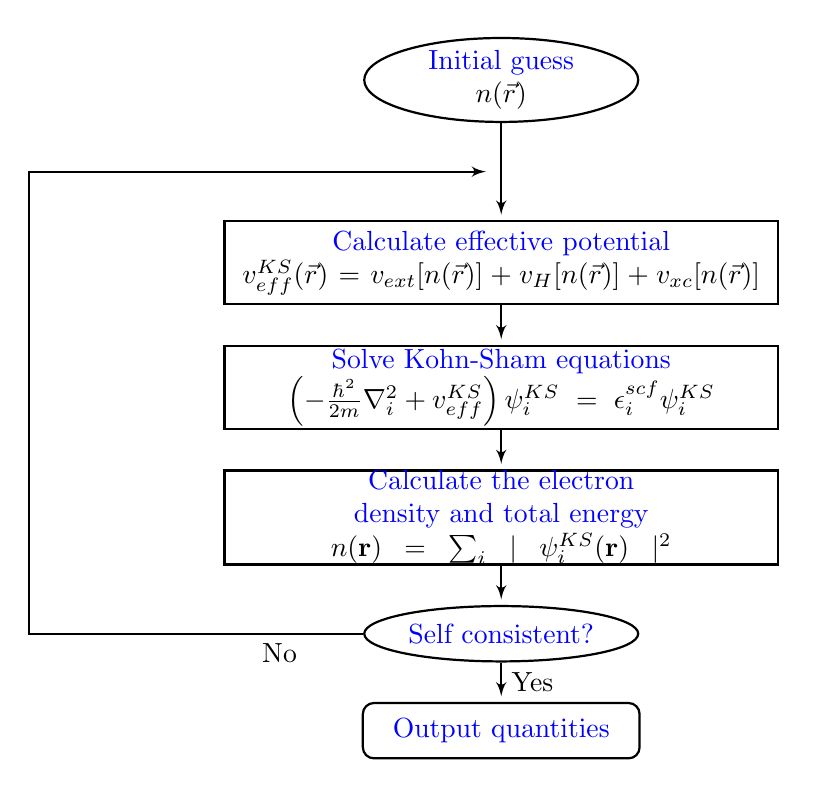
\begin{tikzpicture}[node distance = 2cm, auto]
   \matrix [column sep=2mm, row sep=5mm] {   %%[column sep=2mm, row sep=1mm]
   & \node [cloud] (step1) { \textcolor{blue}{Initial guess} \\ $n(\vec{r})$}  ; & \\
   & \node (null1) {}; & \\
   & \node [block] (step2) { \textcolor{blue}{Calculate effective potential} \\
           $ v^{KS}_{eff}(\vec{r}) = v_{ext}[n(\vec{r})] + v_{H}[n(\vec{r})] + v_{xc}[n(\vec{r})] $}; & \\
   & \node [block] (step3) { \textcolor{blue}{Solve Kohn-Sham equations} \\
           $ \left(-\frac{\hbar^2}{2m}\nabla^2_i+v^{KS}_{eff} \right)\psi^{KS}_i  =\epsilon^{scf}_i\psi^{KS}_i $}; & \\
   & \node [block] (step4) { \textcolor{blue}{Calculate the electron density and total energy} \\ 
           $ n(\textbf{r}) = \sum_i\mid\psi^{KS}_i(\textbf{r})\mid^2   $}; & \\
   & \node [cloud] (step5) { \textcolor{blue}{Self consistent?} }; & \\
   & \node [rect ] (step6) { \textcolor{blue}{Output quantities} }; & \\
   };
    % Draw edges
     \begin{scope} [every path/.style=line]
    \path [line] (step1) -- (step2);
    \path [line] (step2) -- (step3);
    \path [line] (step3) -- (step4);
    \path [line] (step4) -- (step5);
    \path [line] (step5) -- node {Yes}(step6);
    \path [line] (step5) --++ (-6,0) node [near start] {No} |- (null1);
    \end{scope}
 \end{tikzpicture}
 \end{center}
 \caption{Self consistent loop used to solve the KS equations.}
 \label{ks-flow}
 \end{figure}
  
%----------------------------------------------------------------------------------------------------------------

\subsubsection*{Calculation of forces}
\label{force}
\noindent The ``nuclear problem" represented by nuclear SE in equation {\ref{BOA-6}} can be converted into a classical problem by treating the nuclei as classical point objects experiencing a force that is obtained from the gradient of the BO potential energy surface. The information about their dynamics can be obtained by solving Newton's equation of motion. The forces acting on the $K^{th}$ nucleus ($\textbf{F}_K$) is then calculated using the Hellmann-Feynman theorem\cite{Feynman1939, Martin2004} shown below:

\begin{align}
\label{hfforce}
\textbf{F}_K&=-\nabla_{\vec{R}_K} E_{tot}(\textbf{R}) \\
             &=-\int n(\vec{r}) \frac{\partial }{\partial \vec{R}_K} v_{ext}(\textbf{R}) d\vec{r} + \frac{\partial }{\partial \vec{R}_K} v_{nuc-nuc}(\textbf{R})  \\
            &=-\frac{e^2}{4\pi \epsilon_o}\int n(\vec{r})\frac{\partial }{\partial \vec{R}_K}\frac{Z_K}{|\vec{r}-\vec{R}_K|} d\vec{r} - \frac{e^2}{4\pi \epsilon_o} \frac{\partial }{\partial \vec{R}_K} \sum_{\substack {I=1 \\ I\neq K}}^{n_n} \frac{Z_I Z_K}{|\vec{R}_I-\vec{R}_K|}
\end{align}
\noindent

%where $\psi_{\mu e}(\textbf{r};\textbf{R})$ are the electronic eigenstates of electronic Hamiltonian ($H_e$) for a given configuration of $\textbf{R}$, $\textbf{F}_I$ is the force acting on the $I^{th}$ nucleus.



\subsubsection{Quantum Mechanics Molecular Mechanics (QMMM)} \label{qmmm-sec}

\noindent Quantum mechanical solution to the ``electron problem" quite accurately describes the electronic structure properties. An increase in the number of atoms (and therefore electrons) increases the computational cost of the solution. Although DFT is computationally less demanding than the wavefunction-based methods, it is still limited to few hundreds to few thousands of atoms. However, classical solution based on force fields (FF) can handle millions of atoms but at the loss of accuracy in describing electronic properties. As a result, a hybrid scheme coined ``Quantum Mechanics Molecular Mechanics (QMMM)" was introduced which incorporates the best of both worlds.

\noindent In this thesis, additive QMMM based on force-mixing approach is used. Under this approach, the overall system is spatially divided into two subsystems namely, (i) ``Quantum Mechanical subsystem (QM)" : The chemically interesting/important region of the system where the quantum mechanical forces (from DFT) are used to move the atoms, and (ii) ``Molecular Mechanics (MM) subsystem" : The surrounding environment to the chemically important QM region where classical force fields (FF) are used to move the atoms. The additive form of QMMM calculates the total electronic energy in the following manner:
\begin{align}
    \label{QMMM-11}
    E_{tot}^{e, QMMM}=E(QM) + E(MM) + E(QMMM)
\end{align}

\noindent where $E(QM)$ is the total KS energy of the QM atoms calculated from one electron Kohn-Sham Hamiltonian,  $E(MM)$  is the energy of the MM atoms calculated using (modified SPC) FF and $E(QMMM)$ is the coupling energy between the MM and QM atoms given by:   

\begin{align}
    \label{QMMM-2}
    E(QMMM)=E^{bond}_{QMMM}+E^{vdW}_{QMMM}+E^{ele}_{QMMM}
\end{align}

\noindent $E^{bond}_{QMMM}$ is the energy compensation due to link-atom schemes\cite{senn2009qm} when the covalent bond gets severed at the boundary of QM and MM subsystems, $E^{vdW}_{QMMM}$ accounts for the dispersion interactions between the MM and QM atoms and $E^{ele}_{QMMM}$ is the electrostatic interaction between the QM and MM atoms. The electrostatic interaction can be described in multiple ways. Electrostatic embedding, the most commonly used approach (also used in this thesis), incorporates the electrostatic interaction by polarising the one-electron Kohn-Sham Hamiltonian (of the QM atoms) with MM charges. The total QMMM energy using the electrostatic embedding approach is written as:

\begin{align}
    \label{QMMM-3}
    E_{tot}^{e, QMMM}=E^{el-em}(QM) + E(MM) + E^{bond}(QMMM) + E^{vdW}_{QMMM}
\end{align}


\noindent where $E^{el-em}(QM)$ is the total KS energy calculated from the polarised ``QM" Hamiltonian. The atoms can have dynamic movement between the two subsystems. %As a result, the total energy, calculated as a summation of energies of two subsystems and their interaction, violates the energy conservation.  Since, the forces on atoms are calculated separately for the two subsystems, the forces under force-mixing approach become non-conservative. 


\subsection{Nuclear Problem: Quantum to Statistical Mechanics}
\label{nuclear_problem}
\noindent The nuclear SE for the electronic ground state represented  by the ground state Born-Oppenheimer potential ($\hat{V}^{BO}_{nuc,0}(\textbf{R})$) is given as: 

\begin{equation}
    \label{NSE-1}
    \hat{H}_{nuc,0}\Phi^{\mu n}_{0}(\textbf{R}) = (\hat{T}_{nuc} + \hat{V}^{BO}_{nuc,0}(\textbf{R})) \Phi^{\mu n}_{0}(\textbf{R})
\end{equation}

\begin{equation}
    \label{NSE-2}
    \hat{V}^{BO}_{nuc,0}=E^{e}_{0}((\textbf{R}))+\hat{V}_{nuc-nuc}(\textbf{R})
\end{equation}

\noindent As described before the electronic SE was solved using DFT (in Chapter 3) and QMMM (in Chapter 4). However, the nuclear SE can only be solved if the complete information of the Born-Oppenheimer potential energy surface (PES) (corresponding to  $E^{e}_{0}(\textbf{R})$) is known. This would involve calculating the electronic structure energy at $(N_{dx})^{3n_e-6}$ points in the PES, where $N_{dx}$ is the number of discretization (by $dx$) along each nuclear degrees of freedom. Additionally, the ground state nuclear wave function does not portray the complete information of a system in thermal equilibrium as multiple nuclear states get populated.  

\noindent In order to study the system at thermal equilibrium, the necessity to solve the nuclear SE is substituted by sampling the Born-Oppenheimer PES (BO-PES). The sampling of the BO-PES at the electronic ground state is done by first writing the canonical (thermal) partition function (Z). For most systems at ambient conditions, the sampling of BO-PES is carried out by treating the nuclei as classical particles thereby generating the ``Classical Canonical Partition Function". However, for systems with lighter nuclei like H and/or low temperatures the description of the BO-PES through classical nuclei becomes inadequate. In such cases, the representation of the true partition function corresponding to the BO-PES is only achieved by treating the nuclei quantum-mechanically (``Quantum Canonical Partition Function"). In the next subsection, the equations for the classical and quantum canonical partition functions are given. 
%------------------------------------------------------------------------------------------------------------------------------------------------------------------------------

\subsubsection{Classical Canonical Partition Function}

For a system of $n_n$ nuclei, the nuclear position vectors and their respective momenta are represented by $\textbf{R}$ ({$\vec{R}_1,\vec{R}_2,\cdots \vec{R}_{n_n}$}) and $\textbf{P}$ ({$\vec{P}_1,\vec{P}_2,\cdots \vec{P}_{n_n}$}) respectively. The nuclear system is completely described using these $6n_n$ degrees of freedom, commonly known as the ``phase space". The classical behaviour of the nucleus ensures the energy values with respect to position ($\vec{R}$) and momentum ($\vec{P}$) are not quantized for any potential. As a result, the potential and kinetic energy of the system can be separately evaluated. The resulting equation for the classical canonical partition function ($Z^{Cl}(\beta)$, where $\beta= \frac{1}{k_{B}T}$) is as follows:

\begin{align}
    Z^{Cl}(\beta)&=\frac{1}{(2\pi\hbar)^{3n_n}} \int_{}^{}d\vec{P}\int_{}^{}d\vec{R} \quad e^{-\beta H_{nuc,0}(\textbf{P},\textbf{R})}\label{CPF-1-1}\\ 
    &= \frac{1}{(2\pi\hbar)^{3n_n}} \int_{}^{}d\vec{P}\int_{}^{}d\vec{R} \quad e^{-\beta(T_{nuc}(\textbf{P})+ V^{BO}_{nuc,0}(\textbf{R}))}\label{CPF-1-2}\\
    &= \frac{1}{(2\pi\hbar)^{3n_n}} \int_{}^{}d\vec{P}\int_{}^{}d\vec{R}\quad e^{-\beta T_{nuc}(\textbf{P})}e^{-\beta V^{BO}_{nuc,0}(\textbf{R})}\label{CPF-1-3}\\
    &= \frac{1}{(2\pi\hbar)^{3n_n}} \int_{}^{}e^{-\beta T_{nuc}(\textbf{R})} d\vec{P}\int_{}^{}e^{-\beta V^{BO}_{nuc,0}(\textbf{R})}d\vec{R}\label{CPF-1-4}     
\end{align}

\noindent where $H$ is the total energy of the nuclei for a particular set of momenta (\textbf{P}) and positions (\textbf{R}), $T_{nuc}(\textbf{P})$ is the kinetic energy dependent only on \textbf{P} and $V^{BO}_{nuc,0}(\textbf{R})$   is the BO potential energy (of the electronic ground state) dependent solely on \textbf{R}. The separation of the exponential terms in equation \ref{CPF-1-2} is due to the classical nature of the nuclei which allows the commutation of the kinetic and potential energy terms. 

%------------------------------------------------------------------------------------------------------------------------------------------------------------------------------

\subsubsection{Quantum Canonical Partition Function}

The quantum nature of the nuclei ensures that the energy levels of a collection of nuclei are quantized (only for potential generating bound states). As a result, each such energy level is represented by a nuclear wave function which describes the state of the system. At thermal equilibrium, multiple nuclear states are populated using the Boltzmann operator ($e^{-\beta\hat{H}_{nuc,0}(\textbf{P},\textbf{R})}$), where $\hat{H}_{nuc,0}$ is the nuclear Hamiltonian for the electronic ground state and $\beta= \frac{1}{k_BT}$. Therefore, the quantum mechanical partition function for a system of ``$\textit{distinguishable}$" nuclei  ($Z^{Qt}(\beta)$) is written as the trace (Tr) of the Boltzmann operator. 

\begin{align}
    Z^{Qt}(\beta)&=Tr[e^{-\beta\hat{H}_{nuc,0}(\textbf{P},\textbf{R})}]\label{QPF-1-1}\\  
    &=\sum_{\mu n}^{}\bra{\Phi^{\mu n}_{nuc,0}(\textbf{R})} e^{-\beta\hat{H}_{nuc,0}(\textbf{P},\textbf{R})} \ket{\Phi^{\mu n}_{nuc,0}(\textbf{R})}\label{QPF-1-2}\\
    &=\sum_{\mu n}^{}e^{-\beta E_{\mu n}}\label{QPF-1-3}
\end{align}

\noindent However, calculating the trace over $e^{-\beta\hat{H}_{nuc,0}(\textbf{P},\textbf{R})}$ is not straight forward (exactly solvable for only few cases), since the kinetic energy ($\hat{T}_{nuc}(\textbf{P})$) and potential energy ($\hat{V}^{BO}_{nuc,0}(\textbf{R})$) operators do not commute. As a result, the Boltzmann operator becomes non-factorizable in equation \ref{QPF-2-1}. 

\begin{align}
    Z^{Qt}(\beta)&=Tr[e^{-\beta\hat{H}_{nuc,0}(\textbf{P},\textbf{R})}] \notag\\  &=Tr[e^{-\beta(\hat{T}_{nuc}(\textbf{P})+\hat{V}^{BO}_{nuc,0}(\textbf{R}))}]\label{QPF-2-1}\\
    &\neq Tr[e^{-\beta\hat{T}_{nuc}(\textbf{P})}e^{-\beta \hat{V}^{BO}_{nuc,0}(\textbf{R})}]\label{QPF-2-2}
\end{align}


\subsubsection*{Classical Isomorphism}
A practical way to tackle the problem is to transform (Figure \ref{fig:mapping}) each quantum nuclei into a ring polymer of classical pseudo-particles (beads/replicas) . In the ring polymer, each bead is connected to two neighbouring beads by harmonic springs. In the special case of a closed ring polymer, the first bead is connected to the last bead. The representation of a quantum particle as a classical ring polymer enforces (i) the Heisenberg Uncertainty principle which prevents the system to have zero energy at 0 K due to the presence of inter-bead harmonic vibrations and (ii) the wave nature of the nucleus by creating a spread around the centroid of the ring polymer. The spread of the ring polymer is represented in the form of its radius of gyration $r_G$, defined by:
\begin{align}
    \label{ROG-1}
     r_G = \sqrt{\frac{1}{N}\sum_{i=1}^{N} (\vec{R}^i-\vec{R}^c)^2}
\end{align}

\noindent where $\vec{R}^i$ is the position of i$^{th}$ bead of the ring polymer and $\vec{R}^c$ is the centroid of the polymer ($\vec{R}^c=\frac{1}{N}\sum_{i=1}^{N} (\vec{R}^i))$. The radius of gyration, $r_G$, is associated with the thermal de Broglie wavelength ($\Lambda$) of the quantum nucleus. At thermal equilibrium,  the relationship between $r_G(T)$ and $\Lambda(T)$ is given by:


\begin{align}
    \label{QPF-3}
    \langle r_G(T)^2\rangle^{\frac{1}{2}}=\frac{\Lambda(T)}{8\pi}
\end{align}

\begin{figure}
    \centering
    \includegraphics[width=12cm ]{./Comp_methods/Figures/mapping.jpg}
    \caption{The classical isomorphism of a quantum nucleus into a classical ring polymer. The mapping is exact in the limit ${N\to\infty}$.}
    \label{fig:mapping}
\end{figure}


\noindent where the average is over the canonical microstates. An exact description of the quantum  nucleus is only achieved in the limit where the number of beads ($N$) in the ring polymer tends to $\infty$. The interaction among the collection of quantum nuclei is now transformed into an interaction of ring polymers with each bead from one ring polymer interacting with the corresponding beads of other ring polymers. The quantum partition function for the classically isomorphed ring polymers is written below:



\begin{align}
    &Z^{Qt}(\beta)\notag\\
                 &=Tr[e^{-\beta\hat{H}_{nuc,0}(\textbf{P},\textbf{R})}]\label{QPF-7-33}\\ 
                 &=Tr\bigg[\bigg(e^{-\beta_N\hat{H}_{nuc,0}(\textbf{P},\textbf{R})}\bigg)^N\bigg]\label{QPF-7-4}\\
                 &=\lim_{N\to\infty}  \prod_{I=1}^{n_n} (\frac{M_I}{2\pi \hbar^2 \beta_N})^{\frac{3N}{2}} \int_{}^{} \bigg(\prod_{I=1}^{n_n} \prod_{j=1}^{N} d\vec{R}^{j}_{I}\bigg) \quad e^{-\beta_N \sum_{j=1}^{N}    \bigg[\hat{V}^{BO}_{nuc,0}(\textbf{R}^{j})+ \sum_{I=1}^{n_n} \frac{M_I\omega^2}{2}(\vec{R}^{j}_{I}-\vec{R}^{j-1}_{I})^2\bigg]}\label{QPF-7-2}          
\end{align}


\noindent where $n_n$ is the number of nuclei, $M_I$ is the mass of the $I^{th}$ nucleus, $\beta_N=\frac{\beta}{N}$, $\vec{R}^j$ is the position of the $j^{th}$ bead of the ring polymer  and $\omega$ ($= \frac{1}{\beta_N \hbar}$ is the frequency of the harmonic spring between any two beads. The derivation of the quantum partition function (equation \ref{QPF-7-4}) into the partition function of the classical ring polymer (equation \ref{QPF-7-2}) is not mentioned for brevity. However, the derivation includes two prominent quantum mechanical  exploits: (i) the symmetric ``Trotter factorization" of the nuclear Hamiltonian and (ii) the induction of $N-1$ (where $\lim_{N\to\infty}$) position (momenta) eigenstates. The above expression is exact in the limit $N$ tends to $\infty$. However, in order to solve a tractable solution, the value of $N$ needs to be converged. A finite value of $N$ introduces the first approximation to the quantum partition function ($Z_N$) and is given by:

\begin{align}
Z_N&=\prod_{I=1}^{n_n} (\frac{M_I}{2\pi \hbar^2 \beta_N})^{\frac{3N}{2}} \int_{}^{} \bigg(\prod_{I=1}^{n_n} \prod_{j=1}^{N} d\vec{R}^{j}_{I}\bigg) \quad e^{-\beta_N \sum_{j=1}^{N}    \bigg[\hat{V}^{BO}_{nuc,0}(\textbf{R}^{j})+ \sum_{I=1}^{n_n} \frac{M_I\omega^2}{2}(\vec{R}^{j}_{I}-\vec{R}^{j-1}_{I})^2\bigg]}\label{QPF-7-5}
\end{align}
 
 \noindent The classical isomorphism of the quantum nucleus into a classical ring polymer maps the quantum problem into a classical problem of $N$ dimensions. 


\subsubsection*{Imaginary Time Path Integrals}

\noindent A partition function provides the statistical information of the system and is ignorant of the dynamics. However, it is important to understand how the system propagates from one microstate to another. The quantum dynamics of a nuclear system is described by the time dependent nuclear SE with Hamiltonian $\hat{H}_{nuc}$. The evolution of the state of the system from time $t_o$ to $t$ is given by: 

\begin{align}
    \label{QPF-7}
    &i\hbar \frac{\partial}{\partial t}\ket{\Phi(t)}=\hat{H}\ket{\Phi(t)}\\
    &\ket{\Phi(t)} = e^{\frac{-i\hat{H}_{nuc}(t-t_{0})}{\hbar}}\ket{\Phi(t_{0})}=\hat{U}(t)\ket{\Phi(t_{0})}
\end{align}

\noindent where $\hat{U}(t)$ is the quantum time evolution operator. Let us assume, during the time evolution from $t_o$ to $t$, the system moves from $\vec{R}^o$ to $\vec{R}$ such that the state of the system at $\vec{R}$ ($\langle \vec{R} | \Phi(t)\rangle$) is represented as:

\begin{align}
    \label{QPF-8}
      \langle \vec{R} | \Phi(t)\rangle &= \ket{\Phi(\vec{R},t)}\notag\\
      &=\bra{\vec{R}}\hat{U}(t)\ket{\Phi(t_{0})}\notag\\
      &=\int_{}^{}d\vec{R}^o\quad \bra{\vec{R}}\hat{U}(t)\ket{\vec{R}^o}\bra{\vec{R}^o}\ket{\Phi(t_{0})}\notag\\
      &=\int_{}^{}d\vec{R}^o\quad \bra{\vec{R}}\hat{U}(t)\ket{\vec{R}^o}\ket{\Phi(\vec{R}^{o},t_{0})}\notag\\
      &=\int_{}^{}d\vec{R}^o\quad \kappa(\vec{R},\vec{R}^o,t)\ket{\Phi(\vec{R}^{o},t_{0})}
\end{align}

\noindent where $\kappa(\vec{R},\vec{R}^o,t)$ is the ``time evolution amplitude" and forms the heart of the path integral formulation of quantum mechanics. The derivation of $\kappa(R,R^o,t)$ (out of the scope of this thesis) leads to the infinite paths the nuclear system takes to go from ($R^o$ at time $t_o$) to ($R$ at time $t$) which eventually forms the basis of path integrals. The ring polymers can be linked to be the evolution of the path integrals from $R^o$ to $R^o$ in imaginary time  of $\beta\hbar$ time length. The imaginary time propagation is invoked using the Wick rotation of the quantum Boltzmann operator ($e^{-\beta \hat{H}}$). The correlation between the quantum evolution operator ($e^{\frac{-i\hat{H}t}{\hbar}}$) with the Boltzmann operator ($e^{-\beta \hat{H}}$) is shown using the following equivalence:


\begin{align}
    \label{QPF-9}
    \hat{U}(t)=&e^{\frac{-i\hat{H}t}{\hbar}}\equiv e^{-\beta \hat{H}}\notag\\
    &\rightarrow \frac{-i\hat{H}t}{\hbar} =-\beta \hat{H}\notag\\
    &\rightarrow it= \hbar\beta; \quad \beta = it/\hbar
\end{align}

\noindent Hence, the classical isomorphism is also known as the imaginary time path integrals or simply path integrals. 
%------------------------------------------------------------------------------------------------------------------------------------------------------------------------------

\section{Molecular Dynamics (MD) Simulation: Sampling of the BO-PES}
\label{MD}
\noindent The  canonical partition function provides a mathematical representation to the BO-PES at thermal equilibrium. Monte Carlo and Molecular dynamics (MD) are the most common methods to sample any PES. In this thesis, MD is used to sample BO-PES. Depending on the description of the nuclei as quantum or classical, two distinct MD simulations have been used. They are (i) classical nuclei MD, which includes Born-Oppenheimer MD (BOMD) and Quantum Mechanics Molecular Mechanics MD (QMMM MD), and (ii) quantum nuclei MD which includes Path Integral Generalized Langevin Equation based MD\cite{ceriotti2012efficient} (PIGLET). 
%and thermostatted  Ring Polymer MD\cite{rossi2018fine} (t-RPMD). 

\noindent The next subsection very briefly describes the various MD simulation techniques undertaken in this thesis.          
%------------------------------------------------------------------------------------------------------------------------------------------------------------------------------

\subsection{Classical Nuclei MD: Born-Oppenheimer MD (BOMD)}

\subsubsection*{Hamiltonian}

\noindent The nuclear Hamiltonian corresponding to the classical partition function (equation \ref{CPF-1-4}) is  separable and consists of the kinetic ($\hat{T}_{nuc}(\textbf{P})$) and Born-Oppenheimer potential energy ($\hat{V}^{BO}_{nuc,0}(\textbf{R})$) terms. The expression for the classical nuclear Hamiltonian is as follows: 
\begin{align}
    \label{BOMD-1}
    &H^{cl,nuc}=H^{cl}_{kin}+H^{cl}_{pot}\\
    &H^{cl}_{kin}=\hat{T}_{nuc}(\textbf{P}); H^{cl}_{pot}=\hat{V}^{BO}_{nuc,0}(\textbf{R})
\end{align}

\subsubsection*{Propagator}

\noindent The microstates of $Z^{Cl}$ are sampled using a classical propagator. In BOMD simulations, the classical propagation is achieved through the Lagrangian ($\mathcal{L}_{BOMD}$) formulation of classical mechanics, where the Lagrangian ( $\mathcal{L}$) is given by:

\begin{align}
    \label{BOMD-2}
    \mathcal{L}_{BOMD}&=\hat{T}_{nuc}(\textbf{P})-\hat{V}^{BO}_{nuc,0}(\textbf{R})\\ 
                       &=\sum_{I=1}^{n_n}(\frac{M_I\Dot{\Vec{R_I}}^2}{2})-\hat{V}^{BO}_{nuc,0}(\textbf{R})
\end{align}

\noindent $\mathcal{L}_{BOMD}$ is then used in the Euler-Lagrange equation to integrate the equation of motion based on the velocity Verlet scheme.

\begin{align}
    \label{BOMD-3}
    &\frac{d}{dt}\frac{\partial \mathcal{L}_{BOMD}}{\partial \Dot{\Vec{R_I}}} = \frac{\partial \mathcal{L}_{BOMD}}{\partial \Vec{R_I}}\\
%    &\textbf{M}\ddot{\textbf{R}}=\textbf{F}
\end{align}

\noindent The thermostat used to maintain thermal equilibrium in the BOMD simulation is  the ``Canonical Sampling through Velocity Rescaling\cite{bussi2007canonical}" (CSVR). The CSVR thermostat rescales the velocity of all the particles (on the basis of equipartition theorem) so that the temperature of the system remains uniform and constant.  
%------------------------------------------------------------------------------------------------------------------------------------------------------------------------------

\subsection{Classical Nuclei MD : Quantum Mechanics Molecular Mechanics MD (QMMM MD)}

\subsubsection{Hamiltonian}
\noindent As mentioned in section \ref{qmmm-sec} , the system of atoms is divided into two regions (i) the QM  subsystem and (ii) the MM subsystem. Therefore, the nuclear Hamiltonian is modified to incorporate the two subsystems and is given by the following equation:

\begin{align}
    \label{QMMM-MD}
    H_{nuc}^{QMMM}=H^{QM}_{nuc} + H^{MM}_{nuc}
\end{align}

\subsubsection{Propagator}

QMMM MD, alike BOMD, uses the same classical propagator for obtaining the equation of motions. However, the force-mixing scheme of QMMM  uses two sets of forces calculated from the two theories (DFT and FF). Therefore, the Lagrangian for the two subsystem ($\mathcal{L}^{QM}$ and $\mathcal{L}^{MM}$) are different. Moreover, there is dynamic transfer of atoms between the two regions which necessitates the use of a stronger Adaptive Langevin\cite{jones2011adaptive} thermostat. The Adaptive Langevin (Ad-LE) thermostat is a combination of Langevin thermostat  and Nose–Hoover thermostat where the former ensures ergodicity whereas the latter compensates for the loss in energy conservation. The Lagrangian and the equation of motion gets modified in the presence of the Adaptive Langevin thermostat.

\begin{align}
    \label{QMMM-1}
    &\mathcal{L}^{QM}_{Ad-LE}=\mathcal{L}^{QM}+\mathcal{L}_{Ad-LE}\\
    &\mathcal{L}^{MM}_{Ad-LE}=\mathcal{L}^{MM}+\mathcal{L}_{Ad-LE}
\end{align}


%------------------------------------------------------------------------------------------------------------------------------------------------------------------------------


\subsection{Quantum Nuclei MD: Path Integral Generalized Langevin Equation Thermostat (PIGLET)}

\subsubsection{Hamiltonian}

The expression for the canonical partition function for $N$ bead ring polymer ($Z_N$) integrates out the momenta of the nuclei. This form of partition function is sampled using Monte Carlo. However, in order to have a MD simulation, the momenta of the nuclei needs to be re-introduced into $Z_{N}$. The re-introduction of momenta becomes a tool for MD and can be tuned for effective  sampling. The tuning is done by changing the physical mass of the nucleus ($M_I$) with a fictitious one ($\tilde{M_I}$). The equation for $Z_N$ due to the reintroduction of the fictitious momenta is given by:


\begin{align}
    \label{QNMD-1}
    Z_{N}&=\prod_{I=1}^{n_n} (\frac{M_I}{2\pi \hbar^2 \beta_N})^{\frac{3N}{2}} \int_{}^{} \bigg(\prod_{I=1}^{n_n} \prod_{j=1}^{N} d\vec{R}^{j}_{I}\bigg) \quad e^{-\beta_N \sum_{j=1}^{N}    \bigg[\hat{V}^{BO}_{nuc,0}(\textbf{R}^{j})+ \sum_{I=1}^{n_n} \frac{M_I\omega^2}{2}(\vec{R}^{j}_{I}-\vec{R}^{j-1}_{I})^2\bigg]}\notag\\ 
    &=\frac{1}{(2\pi\hbar)^{3n_nN}} \bigg(\frac{\textbf{M}}{\Tilde{\textbf{M}}}\bigg)^{\frac{3N}{2}} \int_{}^{} \bigg(\prod_{I=1}^{n_n} \prod_{j=1}^{N} d\vec{R}^{j}_{I}\bigg) \bigg(\prod_{I=1}^{n_n} \prod_{j=1}^{N} d\vec{P}^{j}_{I}\bigg)\notag\\ 
    & \quad e^{-\beta_N \sum_{j=1}^{N}  \bigg[\hat{V}^{BO}_{nuc,0}(\textbf{R}^{j})+ \sum_{I=1}^{n_n} \frac{M_I\omega^2}{2}(\vec{R}^{j}_{I}-\vec{R}^{j-1}_{I})^2 + \sum_{I=1}^{n_n} \frac{(\vec{P_I}^j)^2}{2\Tilde{M}}\bigg]}\notag\\     
\end{align}

%%%%%%%%%%%%%%%%%%%%%%%%%%%%%%%%%%%%%%%%%%%%%%%%%%%%%%%%%%%%%%%ERROR
   


 \noindent The corresponding Hamiltonian is known as the ``PIMD" Hamiltonian ($\hat{H}^{pimd}_{N,nuc,0}(\textbf{P}^{(j)},\textbf{R}^{(j)})$) where $\textbf{P}^{(j)}$ and $\textbf{R}^{(j)}$ are the set of momenta and position vectors for all beads and nuclei. $\Tilde{\textbf{M}}$ and $\textbf{{M}}$ are the fictitious and physical/real mass matrices of all the nuclei. The associated MD is known as the ``Path Integral Molecular Dynamics (PIMD)". The expression for PIMD Hamiltonian is given below:

\begin{align}
\label{QNMD-2}
    \hat{H}^{pimd}_{N,nuc,0}(\textbf{P}^{(j)},\textbf{R}^{(j)})=\sum_{j=1}^{N}  \bigg[\hat{V}^{BO}_{nuc,0}(\textbf{R}^{j})+ \sum_{I=1}^{n_n} \frac{M_I\omega^2}{2}(\vec{R}^{j}_{I}-\vec{R}^{j-1}_{I})^2 + \sum_{I=1}^{n_n} \frac{(\vec{P_I}^j)^2}{2\Tilde{M_I}}\bigg]
\end{align}

\noindent  However, restricting the choice of the fictitious momenta to the actual momenta of the nuclei constructs the ``RPMD" Hamiltonian ($\hat{H}^{rpmd}_{N,nuc,0}(\textbf{P}^{(j)},\textbf{R}^{(j)})$) and the subsequent ``Ring Polymer Molecular Dynamics (RPMD)". The expression for RPMD hamiltonian is given below: 

\begin{align}
\label{QNMD-3}
    \hat{H}^{rpmd}_{N,nuc,0}(\textbf{P}^{(j)},\textbf{R}^{(j)})=\sum_{j=1}^{N}  \bigg[\hat{V}^{BO}_{nuc,0}(\textbf{R}^{j})+ \sum_{I=1}^{n_n} \frac{M_I\omega^2}{2}(\vec{R}^{j}_{I}-\vec{R}^{j-1}_{I})^2 + \sum_{I=1}^{n_n} \frac{(\vec{P_I}^j)^2}{2M_I}\bigg]
\end{align}

\noindent The terms RPMD and PIMD are used interchangeably in this thesis as both refer to the RPMD Hamiltonian where the real masses of the nuclei are used.

\subsubsection{Propagator}

\noindent In PIMD or RPMD, the microstates of $Z_N$ are also sampled using the classical dynamics of the nuclei. The classical propagation is based on the classical Liouvillian formulation of the Hamiltonian equation of motion. The Hamiltonian equations of motion are as follows: 

\begin{align}
    \label{QNMD-4}
    &\frac{d\textbf{R}^{(j)}}{dt}=\frac{\partial\hat{H}^{rpmd}_{N,nuc,0}(\textbf{P}^{(j)},\textbf{R}^{(j)})}{\partial \textbf{P}^{(j)}}\notag\\
    &\frac{d\textbf{P}^{(j)}}{dt}=-\frac{\partial\hat{H}^{rpmd}_{N,nuc,0}(\textbf{P}^{(j)},\textbf{R}^{(j)})}{\partial \textbf{R}^{(j)}}\notag\\
\end{align}

\noindent The classical Liouvillian propagator ($e^{iLt}$) and its corresponding equations of motion are as follows:

\begin{align}
    \label{QNMD-5}
    &iL=\bigg(\frac{\partial\hat{H}^{rpmd}_{N,nuc,0}(\textbf{P}^{(j)},\textbf{R}^{(j)})}{\partial \textbf{P}^{(j)}}\bigg) \frac{\partial}{\partial \textbf{R}^{(j)}} + \bigg(-\frac{\partial\hat{H}^{rpmd}_{N,nuc,0}(\textbf{P}^{(j)},\textbf{R}^{(j)})}{\partial \textbf{R}^{(j)}}\bigg) \frac{\partial}{\partial \textbf{P}^{(j)}}
\end{align}

\begin{align}
    \label{QNMD-55}
    &\textbf{R}^{(j)}(t)=e^{iLt}\textbf{R}^{(j)}(t_o)\notag\\
    &\textbf{P}^{(j)}(t)=e^{iLt}\textbf{P}^{(j)}(t_o)
\end{align}

\noindent The classical evolution of interacting ring polymers (Eq. \ref{QNMD-55}) is difficult to integrate and is often done in an unexact fashion. Therefore, a more practical way is to split the Hamiltonian into two parts namely (i) Hamiltonian for the free ring polymer ($\hat{H}^{frp}_{N,nuc,0}$) and (ii) Hamiltonian for the potential between the ring polymers ($\hat{H}^{pot}_{N,nuc,0}$) and evolve the individual split up Hamiltonians exactly. Here and after, the dependence of the RPMD Hamiltonian on the position and momenta vectors is dropped for simplicity. The readjusted expression for the complete Hamiltonian is as follows:

\begin{align}
\label{QNMD-6}
    \hat{H}^{rpmd}_{N,nuc,0}&=\hat{H}^{pot}_{N,nuc,0}+\hat{H}^{frp}_{N,nuc,0}\\
                             &=\sum_{j=1}^{N}  \bigg[\hat{V}^{BO}_{nuc,0}(\textbf{R}^{j})\bigg] + \sum_{j=1}^{N} \sum_{I=1}^{n_n} \bigg[\frac{M_I\omega^2}{2}(\vec{R}^{j}_{I}-\vec{R}^{j-1}_{I})^2 + \frac{(\vec{P_I}^j)^2}{2M_I}\bigg]
\end{align}

\noindent Each part of the Hamiltonian is associated with their respective classical propagators obtained approximately by the symmetric Trotter factorization of the complete classical propagator. The resultant equation for the split up classical propagator for a $\Delta t$ time step is as follows:

\begin{align}
\label{QNMD-66}
    &e^{iL\Delta t}\simeq e^{iL_{pot}\frac{\Delta t}{2}}e^{iL_{frp}\Delta t}e^{iL_{pot}\frac{\Delta t}{2}}
\end{align}

\noindent where $e^{iL_{frp}}$ is associated with $\hat{H}^{frp}_{N,nuc,0}$ and $e^{iL_{pot}}$ is associated with $\hat{H}^{pot}_{N,nuc,0}$. The overall algorithm\cite{ceriotti2010efficient} for integrating the equations of motion for a $\Delta t$ is as follows (dropping the vector sign over $\vec{P}$ and $\vec{R}$ for simplicity):

\begin{align}
    &P_I^{j} \leftarrow P_I^{j} - \frac{\Delta t}{2}\frac{\partial V(\textbf{R}^j)}{\partial R_I^j}\label{QNMD-71}\\
    &\Tilde{P_I^{k}} \leftarrow \sum_{j=1}^{N}P_I^{j}C_{jk};\quad \Tilde{R_I^{k}} \leftarrow \sum_{j=1}^{N}R_I^{j}C_{jk} \label{QNMD-72}\\
    &\begin{bmatrix}
        \Tilde{P_I^{k}} \\ \Tilde{R_I^{k}} 
    \end{bmatrix}
    \leftarrow\begin{bmatrix}
        cos (\omega_{k}\Delta t) \quad \quad -M_I \omega_{k} sin (\omega_{k}\Delta t) \\
        \frac{1}{M_I\omega_{k}}sin (\omega_{k}\Delta t) \quad \quad cos (\omega_{k}\Delta t)
    \end{bmatrix}
    \begin{bmatrix}
        \Tilde{P_I^{k}} \\ \Tilde{R_I^{k}} 
    \end{bmatrix}\label{QNMD-73}\\
        &P_I^{k} \leftarrow \sum_{k=0}^{N-1}C_{jk}\Tilde{P_I^{j}};\quad R_I^{k} \leftarrow \sum_{k=0}^{N-1}C_{jk}\Tilde{R_I^{j}} \label{QNMD-74}\\
    &P_I^{j} \leftarrow P_I^{j} - \frac{\Delta t}{2}\frac{\partial V(\textbf{R}^j)}{\partial R_{I}^{j}}\label{QNMD-75}
\end{align}

\noindent The first step (Eq. \ref{QNMD-71}) is the exact propagation of the ring polymer momenta by $\Delta t/2$ time step under the influence of $\hat{H}^{pot}_{N,nuc,0}$. The second step (Eq. \ref{QNMD-72}) is the transformation of the cartesian representation of the ring polymer to the normal mode representation where $C_{jk}$ is the orthogonal transformation matrix for an even N.

\begin{align}
    C_{jk}=
    \begin{cases}
    \sqrt{1/N}, &k=0\\
    \sqrt{2/N}cos(2\pi jk/N),&1\leq k \leq N/2-1\\
    \sqrt{1/N}(-1)^j, &k=N/2\\
    \sqrt{2/N}sin(2\pi jk/N),&N/2+1\leq k \leq N-1
    \end{cases}
\end{align}


\noindent The third equation (Eq. \ref{QNMD-73}) is an exact evolution of the ring polymer through a time step of $\Delta t$ in the normal mode representation under the influence of $\hat{H}^{frp}_{N,nuc,0}$. The normal mode frequency of the ring polymer is given as follows:
\begin{equation}
 \omega_k= 2\omega sin(k\pi/N)   
\end{equation}

\noindent The fourth and fifth steps (Eq. \ref{QNMD-74} and Eq. \ref{QNMD-75}) are the transformation of the ring polymer from the normal mode to cartesian representation and the further propagation of the evolved (cartesian) ring polymer by a $\Delta t/2$ time step under the influence of $\hat{H}^{pot}_{N,nuc,0}$ respectively.

\noindent As mentioned earlier, the quantum partition function is exact in the limit where the number of beads of the ring polymer approaches $\infty$. However, an upper cap on the number of beads is obtained using convergence tests. This converged number of beads is proportional to the maximum frequency of the inter nuclear vibration of the physical system and inversely proportional to the temperature ($N \propto \frac{\omega_{max}}{T}$). As a result, at low temperatures and/or high physical vibration, the number of beads needed for converging physical properties becomes large. An efficient way to accelerate the convergence with respect to the number of beads is to couple the RPMD dynamics with a non-equilibrium coloured noise Langevin dynamics\cite{ceriotti2010novel,ceriotti2010efficient,ceriotti2012efficient} that introduces frequency dependent quantum fluctuations to mimic the zero point energy of the system consisting of multi-dimensional harmonic oscillators which also applies to anharmonic systems\cite{ceriotti2011accelerating}. This state of the art thermostatting technique by a non-equilibrium Generalized Langevin equation based thermostat (GLET) of the RPMD simulation is known as Path Integral Generalized Langevin Equation Thermostat\cite{ceriotti2012efficient} (PIGLET). The coupling of the GLET dynamics with the RPMD dynamics modifies the Liouvillian (Eq. \ref{QNMD-66}) in the following manner:  

\begin{align}
\label{QNMD-666}
    &e^{iL\Delta t}\simeq  e^{iL_{GLET}\frac{\Delta t}{2}} e^{iL_{pot}\frac{\Delta t}{2}}e^{iL_{frp}\Delta t}e^{iL_{pot}\frac{\Delta t}{2}} e^{iL_{GLET}\frac{\Delta t}{2}}
\end{align}

\noindent This results in introducing thermostat dynamics twice per step, immediately before and immediately after the RPMD dynamics (Eq. \ref{QNMD-71}-\ref{QNMD-75}). A very brief description regarding the stochastic dynamics is presented below. 

\subsubsection{Generalized Langevin Equation based Thermostat: Stochastic dynamics}

Thermostats are used as temperature control to sample the canonical distribution of positions and momenta of atoms in classical (Newtonian) dynamics. Since ring polymers make the system stiff, Noose-Hoover chain thermostat\cite{martyna1992nose,tuckerman1993efficient} is generally used with RPMD dynamics to obtain ergodicity and is considered a gold standard for perofming path integral molecular dynamics. The Noose-Hoover chain dynamics is detrministic and is applied immediately before and immediately after the RPMD dynamics and is reported elsewhere\cite{ceriotti2010efficient}. Alternatively, Ceriotti and Parinello\cite{ceriotti2010efficient} showed a simple stochastic (white/Markovian) Langevin thermostat, primarily used to model brownian motion, can also be used with path integral simulation (PILE) to ensure ergodicity. The equations of motion for the Langevin dynamics are given below, which similar to Noose-Hoover chain are applied immediately before and after the RPMD dynamics (Eq. \ref{QNMD-71}-\ref{QNMD-75}). 

\begin{align}
    \label{QNMD-91}
     &\Tilde{P_I^{k}} \leftarrow \sum_{j=1}^{N}P_I^{j}C_{jk}\notag\\
      &\Tilde{P_I^{k}} \leftarrow c_1^{k}\Tilde{P_I^{k}} + \sqrt{\frac{M_I}{\beta_N}}c_2^{k}\xi_I^{k}\notag\\ 
      &{P_I}^{j} \leftarrow \sum_{k=0}^{n-1} C_{jk} \Tilde{P_I^{k}}
\end{align}

\noindent where $\xi_I^{k}$ is an independent Gaussian number (random noise term). The coefficients $c_1^{k}$ and $c_2^{k}$ can be written as as follows:

\begin{equation}
    c_1^{k}=e^{(-\Delta t/2)\gamma^{k}} ; \quad  c_2^{k}=\sqrt{1-[c_1^{k}]^2}\label{QNMD-92}\\    
\end{equation}

\noindent where $\gamma^{k}$ is the normal mode friction coefficients. In the view of optimal sampling of the free (non-interacting) ring polymers, $\gamma^{k}$ is given as follows:

\begin{align}
    \label{QNMD-922}
    &\gamma^{k}=
    \begin{cases}
    \sqrt{1/\tau_{0}}, &k=0\\
    2\omega_{k}, &k > 0\\
    \end{cases}    
\end{align}

 \noindent In this approach, the ring polymer normal mode is separated into the centroid ($k=0$) mode with an autocorrelation time of $\tau_0$ and excited modes ($k > 0$) with an autocorrelation time constant of  $2\omega_k$ where $\omega_k$ is the ring polymer frequency of the excited modes. 

 \noindent However, Ceriotti and coworkers showed that a coloured noise (non-Markovian with a memory kernel) Generalized Langevin Thermostat\cite{ceriotti2009langevin} instead of the simple Langevin thermostat gives more control over the static and dynamical properties. This was achieved by converting the non-Markovian (memory) dynamics into a Markovian one\cite{ceriotti2010novel} by extending the phase space with additional momenta bilinearly coupled to the physical momentum. This control over the dynamics prompted Ceriotti and coworkers\cite{ceriotti2009nuclear} to  include quantum corrections to the classical dynamics. They fit the correlation function of the random noise to match the quantum fluctuations in position and momenta of the various vibrational modes of the system in such a way that minimal apriori knowledge about the system is required. As a result of this fitting procedure, the preservation of equivalence between the friction and noise terms, as dictated by the fluctuation-dissipation theorem, is compromised, leading to the emergence of non-equilibrium dynamics. The equation of quantum fluctuations for the position and momentum has the following form.

  \begin{equation}
    c_{RR}(\omega) = \frac{1}{\omega^2} c_{PP}(\omega) = \frac{\hbar}{2\omega} coth \frac{\hbar \omega}{2k_BT} \label{QNMD-97}    
\end{equation}


\noindent where $\omega$ is the frequency of the normal mode, $c_{RR}$ and $c_{PP}$ are the quantum mechanical thermal expectation value of the squared position ($R^2$) and momenta ($P^2$) respectively. This quantum thermostat (QT) was coupled to path integral methods\cite{ceriotti2011accelerating} in order to compliment the remainder quantum fluctuations incorporated using the ring polymer. The corresponding equation of motion is analytically solvable if the physical vibrations in the system are within the harmonic limit but are successfully extended to strongly anharmonic systems\cite{ceriotti2011accelerating} through numerical solutions. The corresponding equations of motions for the PI $+$ GLE method before and after the RPMD dynamics are as follows: 
%\begin{equation}
%    \frac{1}{P} \sum_{k=0}^{N-1}c_{RR}(\omega) = \frac{\hbar}{2\omega} coth \frac{\hbar \omega}{2k_BT} \label{QNMD-98}
%\end{equation}

\begin{equation}
\mathbf{P_{I}^{j}} \leftarrow \mathbf{C_1} \mathbf{P_{I}^{j}} + \sqrt{\frac{M_I}{\beta_{N}}} \mathbf{C_{2}} \boldsymbol{\xi_{I}^{j}} \notag
\end{equation}


\begin{equation}
    \textbf{P}_I^{j} = 
    \begin{bmatrix}
        P_I^{j} \\ \textbf{s}_I^{j}
    \end{bmatrix} \label{QNMD-95}
\end{equation}

\noindent where $\textbf{P}_I^{j}$ is the column vector containing the momentum of the $I^{th}$ nuclei for the $j^{th}$ bead and its additional momenta ($\textbf{s}_I^{j}$;\quad $s_{I,1}^j$ , $s_{I,2}^j$ , ...,$s_{I,n_s}^j$) for enforcing Markovian dynamics in extended phase phase. $\boldsymbol{\xi_{I}^{j}}$ is a vector of $n_s + 1$ independent Gaussian numbers. The $\textbf{C}_1$ and $\textbf{C}_2$ are matrices related to the friction and noise terms respectively and are fitted to enforce quantum fluctuations in the position and momenta. They depend on the number of beads, the additional momenta needed to extend the phase space, the temperature and the highest physical frequency of the system along with the range of frequency in which the quantum corrections are to be applied. The expression and details regarding the matrices, the equations of motion and the fitting procedure can be found in the thesis\cite{ceriotti2010novel} and related publications\cite{ceriotti2012efficient,ceriotti2011accelerating} by Michele Ceriotti (\underline{https://www.epfl.ch/labs/cosmo/}).


%\begin{equation}
%    \textbf{C}_1 = e^{(-\Delta t/2)\gamma^{T}}; \quad \textbf{C}_2^{T}\textbf{C}_2 = I- \textbf{C}_1^{T}\textbf{C}_1 \label{QNMD-94}
%\end{equation}

%\begin{equation}
%    \textbf{P}_I^{j} \leftarrow \frac{-\partial V(\textbf{R}^j)}{\partial R_I^j} + \textbf{C}_1\textbf{P}_I^{j} + \sqrt{\frac{M_I}{\beta_N}}\textbf{C}_2\textbf{\xi}_I^{j} \label{QNMD-96}
%\end{equation}

\noindent Further, it was observed that the PI $+$ GLE method consists of the quantum kinetic energy which is dependent on the centroid mode of the ring polymer leading to bead-bead correlations which slows down its convergence with respect to the number of beads. The solution to this problem was addressed by Ceriotti and coworkers\cite{ceriotti2012efficient} by coupling a classical (equilibrium) thermostat to the centroid mode of the ring polymer and applying to each other normal mode of the ring polymer with the non-equilibrium frequency dependent GLE thermostat. This method ensures the fast convergence of both the potential and quantum kinetic energy with respect to the number of beads and is the ``\textbf{PIGELT}" method used in this thesis. The $\textbf{C}_1$ and $\textbf{C}_2$ matrices obtained through the fitting procedure is freely available at \underline{http://gle4md.org/}. This PIGLET method with respect to PIMD has been successful in reducing the number of beads by a factor 4 and more\cite{ceriotti2010efficient} for structural properties. For water at 300 K, the structural properties are converged over 6 beads of PIGLET compared to the 32 beads for PIMD\cite{ceriotti2012efficient}. Other noticeable example is the structural description of the Zundel cation at low temperatures is strongly benefitted from the use of PIGLET simulation\cite{schran2018converged}. The authors also compare PIGLET with another variant of quantum thermostatting with PIMD named Path Integral Quantum Thermal Bath (PIQTB\cite{schran2018converged,brieuc2016quantum}). 




%%% Thesis chapter1 --------------------------------------------------
\chapter{Effect of Quantum Delocalization on Temperature 
Dependent Double Proton Transfer in Molecular Crystals of Terephthalic Acid } \label{chapter1}
%\footnotetext{Reprinted (adapted) with permission from \emph{Surface Science}, \textbf{2016}, 644, 69-79.}
\ifpdf
    \graphicspath{{Chapter1/Chapter1Figs/}}
\fi
 
% ------------------------------------------------------------------------
\section{Introduction}
\label{intro}

Multiple hydrogen/proton transfer (MPT) reactions play a crucial role in a variety of important processes. The replication of DNA, one of the most fundamental biological  processes, is prone to mutations,\cite{jacquemin2014assessing} which are created by complex steps involving MPTs. MPTs also have a prominent role in enzyme catalysis\cite{kirby1997efficiency,blomberg2006different,richard2012paradigm} as well as in other non-biological systems such as ionic liquids\cite{yoshizawa2003ionic} and organic solids\cite{horiuchi2008organic}. Moreover, the transfer of protons can also be coupled to changes in the underlying electronic structure of the system as seen in proton-coupled electron transfer reactions (PCET).\cite{huynh2007proton,costentin2010update,hammes2010theory,dempsey2010proton,warren2010thermochemistry} PCET reactions are ubiquitous and diverse. For example, excited state proton transfer\cite{arnaut1993excited,zhou2018unraveling}, has potential applications for use as a fluorescent probe\cite{sedgwick2018excited} in biological imaging\cite{yang2014macro} and also for use as an organic opto-electronic material\cite{kwon2011advanced}.

Majority of the MPTs are found in organic molecules like DNA base pairs\cite{watson1953molecular} and their analogues\cite{douhal1995femtosecond,ogawa2000phototautomerizable,abou2001tautomerization}, porphyrin\cite{storm1972nitrogen}, porphycene\cite{waluk2017spectroscopy}, phthalocyanines\cite{liljeroth2007current}, and carboxylic acids\cite{loerting1998toward} where the transfer of two protons generate tautomers. This special category of proton transfer induced tautomerization\cite{antonov2013tautomerism} is classified as double proton transfer (DPT). Depending on the manner in which the two hydrogen atom transfers, the overall process can have two mechanisms namely stepwise or concerted. Typically, a stepwise proton transfer involves individual hydrogen atoms/protons moving separately resulting in metastable intermediates. For example, Zewail and coworkers reported the hydrogen atoms of 7-azaindole dimers\cite{douhal1995femtosecond}, a prototypical system to the DNA base pair, transfer in a non-concerted manner generating ionic intermediate species. On the contrary, Kasha and coworkers\cite{catalan1999resolution} interpret the transfer of protons to have a concerted mechanism where the protons are transferred simultaneously resulting in a single non-ionic transition  state. The stepwise process involves charged intermediates and in most cases, have higher activation barriers whereas the concerted pathway suffers from the small kinetic pre-factor of two atoms transferring at the same time. The competition between the two processes determine the rate of tautomerization and the proportion of tautomers, which are essential in enzymatic reactions\cite{zhu2016tautomerization} and drug delivery\cite{wojnarowska2016tautomerism}.

Since hydrogen atoms are the lightest ones in the periodic table, their structural and dynamical properties are strongly influenced by nuclear quantum effects (NQE). NQEs in DPT processes are typically manifested through zero-point energy and tunnelling. While the zero-point energy fluctuations usually affect free energy barriers, tunnelling facilitates classically forbidden pathways at lower temperature. These manifestations in DPT are not only of fundamental interest in biological processes\cite{klinman} but are equally important in other chemical reactions\cite{nqerect, nqebio}. For example, Ivanov et al.\cite{ivanov2015quantum} and Wikfeldt et al.\cite{wikfeldt2014communication} used path integral molecular
dynamics (PIMD) simulations to capture NQEs in the dimer of formic acid and anti-ferroelectric squaric acid crystals respectively. They find the intermolecular DPT occurs through concerted proton transfer and is temperature dependent. Similarly, Cahlik et al.\cite{cahlik2021significance} using a combination of low temperature STM, atomic force microscopy (AFM) and PIMD simulations,  showed that the transferring hydrogen atoms in the one-dimensional quinonediimine molecular networks supported on Au(111) surface, are concerted. This promotes a delocalization of $\pi$-electrons along the molecular chain  providing enhanced mechanical stability and giving rise to new states in the gap. 
In the study on intramolcular DPT in a single molecule of porphycene,  Litman et al.\cite{porphycene_th} using PIMD simulations report the hydrogen atoms tunnel concertedly at low temperatures ($<$ 100 K) whereas a competition between the concerted and stepwise pathway is observed at high temperatures (100-300 K). Although these studies have provided novel and invaluable information regarding the nature of DPT, we note that most of these studies are primarily cases where the effect of crystal environment have been either ignored by taking single molecule and dimer or partially incorporated through a chain of molecules. However, a complete description of crystal field, much like solvent effects\cite{kwon2007double}, is necessary. One of the discernible effect of crystal field is the non-degeneracy of the tautomers caused due to the induced asymmetry of the potential energy surface.\cite{meier1982structure} The non-degeneracy manifests by modifying the rates of tautomerization which are critical in systems where the proton transfer processes are controlled by external stimuli such as electric field, light, heat, and stress\cite{wang2021stimuli}.

These fascinating reports prompted us to undertake a theoretical study on the nature of DPT. Therefore, in this work we investigate DPT in molecular crystals of terephthalic acid (TPA). The choice provides a more realistic and less complicated system to understand the nature of DPT and how it is modulated by the environment. TPA is also used as a commercial precursor in the polymer industry\cite{fadzil2014brief}. Moreover, the molecules of TPA are used as ligands\cite{decker2020mof,mateo2019long} for synthesizing metal-organic frameworks and supramolecular complexes catering to a wide range of applications.\cite{zhou2012introduction} More recently, Karothu and coworkers\cite{karothu2016shape} observed that the application of thermal/mechanical stimulus on the crystals of TPA results in a polymorphic phase transition\cite{karothu2016shape,ahmed2019shape}. This behaviour is referred to as thermosalient/mechanosalient effect and has important applications in the design of transducers. 

TPA exhibits three crystalline forms, namely, form I, II and III\cite{bailey1967crystal, sledz2001new} of which form I is found to be stable till 500 K\cite{sledz2001new}. When form I is heated from low temperature to room temperature, it is known to undergo a continuous order-disorder transition.\cite{fjaer1986order, fischer1986structure} From their neutron diffraction studies, Fischer and co-workers determined the onset of disorder in the H positions to be around 80 K.\cite{fischer1986structure} Their results were further corroborated by temperature dependent Raman studies by Fjaer and coworkers.\cite{fjaer1986order} The temperature dependence of the disorder is examined using solid state nuclear magnetic resonance  (SS-NMR)\cite{meier1986structure,meier1982structure}. The dipolar lineshapes and relaxation rate measurements find the proton to dynamically exchange in an asymmetric potential. The temperature dependence of relaxation rate at high temperature was explained using chemical kinetics whereas at low temperature, a quantum mechanical tunnelling model was needed. The proton transfer barriers at low (high) temperature were inferred as 8 (27) meV. Similar values of barriers were estimated by Meier and coworkers\cite{meier1983neutron} from their inelastic neutron scattering studies. The authors commented that the small value of activation barrier at low temperature could be the energy difference between the vibrational ZPE of the two minima and emphasized the need for further examination.

Using Born Oppenheimer Molecular dynamics (BOMD) simulations and Path Integral Molecular Dynamics (PIMD) simulations coupled to the Generalized Langevin Equation based thermostat (PIGLET) we have studied the temperature dependent behaviour of NQEs on the DPT in form I of TPA. Our findings show that NQEs involve a tunnelling DPT mechanism at low temperatures ($<$ 100 K) whereas at room temperature (300 K), it is the zero-point energy fluctuations that increases the shuttling process by decreasing the activation barrier. Moreover, we observed that the DPT is concerted throughout the temperature range (70-300 K) where, as expected, the hydrogen atom shuttles like a proton. The rest of the chapter is divided as follows: in Section~\ref{compdet} we provide the details of the BOMD and PIMD simulations. The results are presented and discussed in Section~\ref{results}. Finally, we conclude in Section~\ref{concl} with some outlook and perspectives.


\section{Computational details}
\label{compdet}

Since form I is a stable polymorph of TPA between 70 and
300 K,\cite{sledz2001new, bailey1967crystal} the
temperature range of interest in this study, we have restricted our calculations
to form I. The crystal structure of this form was taken from the Cambridge 
Crystallographic Data Centre under the deposition number 1269122 and is optimized 
using the Broyden–Fletcher–Goldfarb–Shanno\cite{fletcher2013practical} (BFGS) algorithm where the electronic structure was calculated using the
Quickstep\cite{vandevondele2005quickstep} module, which is a Gaussian and Plane 
wave (GPW) based implementation of Density Functional Theory, in the open source 
CP2K\cite{hutter2014cp2k} package. The electronic exchange and correlation are
approximated within the generalized gradient approximation (GGA) framework proposed by 
Becke-Lee-Yang-Parr\cite{becke1988density,lee1988development} (BLYP). van der Waals 
interactions have been included using the Grimme's D3 
dispersion correction\cite{grimme2010consistent}. The electron-ion  
interactions were described by the norm-conserving, separable, dual-space 
Gaussian-type pseudopotentials of Goedecker, Teter, and 
Hutter\cite{goedecker1996separable} (GTH). The triple-zeta valence polarisation
(TZVP) basis set was used to expand the electronic wavefunctions. The 
charge density was expanded on a grid with a plane wave cutoff of 450 Ry. The 
electronic calculations were done using a 2$\times$2$\times$5 supercell. Brillouin zone integrations have been performed using only the $\Gamma$-point.

 
The BOMD simulations of TPA crystals were performed at 70, 100, 200 and 300 K
using a canonical sampling through velocity rescaling\cite{bussi2007canonical}(CSVR) 
thermostat as implemented in the CP2K package.
In order to study the effect of NQE, we have performed PIMD simulations at the same
temperatures. These simulations were carried out using the 
i-PI\cite{kapil2019pi} and CP2K software, where i-PI propagates the nuclear motion 
and CP2K calculates the electronic forces and energy. A coloured noise Generalised 
Langevin Equation based thermostat (GLE) is coupled to PIMD 
simulation\cite{ceriotti2012efficient} (PIGLET) to accelerate the convergence 
with respect to the number of beads. The converged number of beads for the 
PIGLET simulation at 70 K was estimated to be 16 (the results of the convergence tests are shown in 
Section \ref{convergence_si} of the Appendix \ref{appendix4}). For the higher temperature simulations we have used, for consistency, the same number of beads. The parameters for the diffusion and drift matrices of the coloured noise thermostat were generated from the online repository (\emph{http://gle4md.org/}) such that the maximum physical frequency lie close to 4000 cm$^{-1}$ for all
temperatures. The equations of motion in the various molecular dynamics simulations were integrated with a time step of 0.5 fs. The BOMD and PIGLET simulations were performed for 35 ps and 20 ps respectively. The analysis were done using the last 30 ps and 18 ps
of the BOMD and PIGLET trajectories respectively.
 
\section{Results}
\label{results}

\subsection{Crystal Structure of TPA}

Each TPA molecule consists of a benzene ring with two carboxyl group at each of
the para positions of the benzene ring (Figure \ref{fig:str_ptc}(a)). In the crystalline form, the 
molecules are arranged in chains that are formed through double hydrogen bonding
between the hydroxyl OH groups of the -COOH group of one TPA unit with the oxygen of the -COOH group in the 
neighbouring TPA unit. Two such chains are further bound together by weak H 
bonds between the H atoms of the phenyl group and the O atoms of the -COOH group
to give rise to a two-dimensional sheet. These two-dimensional sheets are
stacked on top of each other to give rise to the three-dimensional crystal
structure. Depending upon how two such
sheets are stacked, TPA exists in three polymorphs, namely form I, II and III, where, in case of the most stable form I (see Section \ref{form-si} of the Appendix \ref{appendix4} ), the TPA molecules of one sheet are on top of those
in the sheet below it, as shown in Figure~\ref{fig:str_ptc}(a). 

At 0K, the TPA molecules in form I are in the trans configuration (Figure~\ref{fig:str_ptc}(a)). This is also known as the L-tautomer.
When all the protons of the L-tautomer are transferred to the acceptor O atoms,
another configuration, namely the R-tautomer, can be formed
(Figure~\ref{fig:str_ptc}(b)). Both the tautomers crystallize in the triclinic form with the chain axis parallel to the $a$ lattice vector.
The former is about 19 meV/TPA molecule lower in energy than the latter.
For both the tautomers we obtain the same lattice parameters
($a$, $b$ and $c$ of 9.62, 7.61 and 3.62 \AA~respectively and
$\alpha$, $\beta$ and $\gamma$ of 73.80, 105.07 and 139.44$^{\circ}$
respectively). The lattice parameters obtained from our calculations
are given in Table \ref{tab:0K_str} of the Appendix \ref{appendix4} showing consistency with previous reports\cite{bailey1967crystal,sledz2001new}.

\begin{figure}
    \centering
    \includegraphics[width=16cm ]{./Chapter1/new_figures/structure_ptc.jpg}
    \caption{Crystal structure of form I of TPA using ball and stick 
    representation. Top view showing the stacking of the TPA chains in
    (a) L-tautomer and (b) R-tautomer. The red (yellow) square highlights the strong (weak) inter-molecular H-bonds that result in the formation of the chains (sheets).
    (c) The proton transfer coordinates
    $\delta_1$ and $\delta_2$ at a junction of two TPA molecules. In (a)
    and (b) the topmost layer atoms are shown with solid spheres and the bottom 
    layer atoms are shown as points. In this and the subsequent figures green, red and white spheres represent carbon, oxygen and hydrogen atoms respectively.}
    \label{fig:str_ptc}
\end{figure}

The TPA tautomers have two types of local interactions, (i) a pair of O-H$\cdots$O bond parallel to the chain direction (highlighted by a black square in Figure~\ref{fig:str_ptc}(a) and (b)), with a shorter heavy atoms separation of 2.63 \AA~in both the tautomers and (ii) a pair of C-H$\cdots$O bonds\cite{gu1999fundamental} perpendicular to the chain direction (highlighted by a yellow square in Figure~\ref{fig:str_ptc}(a) and (b)) with heavy atoms separation ($d_{C\cdots O}$) of 3.36 \AA{}  and 3.46 \AA{} in the L-tautomer where the shorter (longer) heavy atom separation is due to the interaction of the benzene hydrogen with the lone pair of the more (less) acidic \textit{sp$^3$} (\textit{sp$^2$}) hybridized carboxyl oxygen. The corresponding $d_{C\cdots O}$ in the R-tautomer are 3.42 \AA{} (where O is \textit{sp$^2$} hybridized) and 3.38 \AA{} (where O is \textit{sp$^3$} hybridized). On the basis of the heavy atom separation\cite{arunan2011definition,desiraju2001weak}, the O-H$\cdots$O is categorised as a strong hydrogen bond (sHB) whereas the C-H$\cdots$O falls under the category of \emph{improper} hydrogen bond. The \emph{improper\cite{van2001nature}} hydrogen bond are weak (wHB) hydrogen bonds which causes blue shift in the covalent bond ($C-H$) stretching. The dissimilar pairs of C-H$\cdots$O wHBs for the L and R-tautomer is responsible for lifting the degeneracy between the two tautomers. As a result, the associated DPT process occurs through a asymmetric double well potential which is discussed in Section \ref{whb-td} of the Appendix \ref{appendix4}.


\subsection{Finite Temperature NQE on strong hydrogen bonds} 

In order to analyze the proton transfer events, we define the following proton transfer coordinates ($\delta_{1,2}$) as shown in Figure \ref{fig:str_ptc}(c), where $\delta_{1,2}$ is the difference
between H-bond length between the acceptor oxygen atom and the transferring hydrogen atom ($d_{O\cdots H}$) and the covalent bond length between the donor oxygen atom and the same transferring hydrogen atom ($d_{O-H}$). At 0 K, in the L-tautomer of form I, the protons are bonded to the donor oxygen atoms and exhibits the ordered state resulting in a negative value of $\delta_{1,2}$. Fluctuations of the $\delta_{1,2}$ between positive and negative values indicate the occurrence of proton transfer events. 


\noindent \textit{Stepwise versus concerted DPT.} The dependency between $\delta_{1}$ and $\delta_{2}$ provides insight into the underlying DPT process. Therefore, in order to understand the the DPT mechanism (stepwise or concerted) and the temperature dependence of NQEs, we have plotted the effective free energy ($F_{eff}$) corresponding to the joint  probability distribution function (JPDF) between the $\delta_1$ and $\delta_2$ (Figure~\ref{fig:delta1_delta2}) at 70 and 300 K for the BOMD and PIGLET simulations. The free energy ($F$) corresponding to a discrete and normalized JPDF ($p$) between two quantities $X$ and $Y$ at ($X_i$, $Y_j$) can be written as: 

\begin{equation}
   F(X_i,Y_j) = -k_{B}T \; ln[\;p(X_i,Y_j) \; dX\;dY] 
    \label{free_energy}
\end{equation}

\noindent where $k_B$ and $T$ are the Boltzmann constant and the simulation temperature, respectively. $p(X_i,Y_i)$ is the normalized JPDF of $X$ and $Y$ at $X_i$ and $Y_j$ respectively. $dX$ and $dY$ are the binning widths used to discretize the $X$ and $Y$ variables respectively. The minima of the discrete free energy surface correspond to the maxima of the joint probability. The effective free energy ($F_{eff}(X_i,Y_j)$) is computed by shifting all $F(X_i,Y_j)$ with the $F^{min}(X_{min},Y_{min})$ as shown in the 
equation below:

\begin{equation}
 \label{free_energy_eff}
 F_{eff}(X_i,Y_j) = F(X_i,Y_j) - F^{min}(X_{min},Y_{min})
\end{equation}

Stepwise proton transfer events will result in local minima in the free energy plots at all the four quadrants since sequential transfers, in addition to the two tautomers at the first and third quadrants, will also generate the (two) ionic intermediates at the second and fourth quadrants. At 70 K, for the classical nuclei,
since there are no proton transfer events, we observe a single local minima
in the third quadrant (Figure~\ref{fig:delta1_delta2}(a)).
Upon increasing the temperature to 300 K, we find minima in both the 
first and third quadrant (Figure~\ref{fig:delta1_delta2}(b)) showing that finite temperature induces concerted proton transfer events.

When the NQE are turned on, local minima of FES are observed in the first and third 
quadrant even at 70 K (Figure~\ref{fig:delta1_delta2}(c)). This of course implies that the proton is significantly more delocalized along the hydrogen bonds fully consistent with previous studies reporting this effect in numerous other organic molecular systems\cite{fang2016inverse,li2011quantum,wang2014quantum,ivanov2015quantum,wikfeldt2014communication,litman2019elucidating,sappati2016nuclear,rossi2016anharmonic,pinotsi2016proton,law2015role,tuckerman1997quantum}. Furthermore, the free energy profile extends to the second and 
fourth quadrant forming an \emph{elbow} suggesting that there are events where both the transferring 
protons are on the same molecule. We note that the presence of such configurations
are indications of occurrence of step-wise proton transfers. However,
since these are higher in energy, their occurrences are rare. Further,
we did not observe any local minima in the \emph{elbow} regions of the free energy profile, which would be
characteristic of step-wise proton transfer. All in all, these results suggest that the DPT in the TPA crystal is primarily a concerted process.

\begin{figure}
\centering
\includegraphics[width=14cm ]{./Chapter1/new_figures/prob_delta1_delta2.jpg}
\caption{The effective free energy ($F_{eff}$) as a function of the proton transfer
coordinates $\delta_1$ and $\delta_2$ at
70 (left column) and 300 K (right column). The top and bottom row are
from BOMD and PIGLET simulations respectively.}
\label{fig:delta1_delta2}
\end{figure}

Upon increasing the temperature to 300 K, we find an enhanced proportion of events in the first quadrant suggesting an increase in proton transfer activities. This symmetrizes the shape of the FES in the first and the third quadrant indicating that at this temperature the disorder in the hydrogen bond network is almost complete. Additionally, the spread of the free energy profile decreases (the \emph{elbow} observed at 70 K softens) along the $\delta_1 = -\delta_2$ direction. This implies that at higher temperatures the probability of finding the configurations where both the protons are on the same molecule is diminished. This behaviour is linked to the loss of correlation between the two transferring protons due to quantum tunneling at 70 K and is discussed in section \ref{losss} of the appendix \ref{appendix4}.
 

\noindent \textit{Quantum tunnelling versus activated hopping.} Our simulations also allow for disentangling the relative role of quantum tunnelling vs activated proton hopping driven by zero point energy fluctuations. The relative role of these two effects will naturally be temperature dependent. The effect of quantum tunnelling can be quantified by an increase in the radius of gyration of the ring polymer representing the quantum nucleus\cite{ceriotti_hbond_fluc}. The radius of gyration probes the quantum uncertainty in position of the nucleus and is proportional to the thermal de Broglie
wavelength of that nucleus. Hence, it is expected that a proton transfer
event due to tunnelling is to be accompanied with an enhancement of the radius of gyration of the proton. Therefore, to examine the extent of this effect, we have computed the radius of gyration, $r_G = 
\sqrt{\frac{1}{P}\sum_{i=1}^{P} (\mathbf{r_i^H}-\mathbf{r_c^H})^2}$,  where H is the hydrogen atom,
$P$ is the number of beads in the ring polymer, $\mathbf{r_i^H}$ is the position of the H-atom in the $i^{th}$ 
bead of the proton ring polymer and $\mathbf{r_c^H}$ is the position of the centroid of the proton ring polymer 
($\mathbf{r_c^H}=\frac{1}{P}\sum_{i=1}^{P} (\mathbf{r_i^H)}$).

Figure~\ref{fig:tunnel2}(a) and (b) shows the proton 
transfer coordinate of the centroid of the ring polymer ($\delta_o^C$; blue graph) and its radius of gyration  ($r_G$; red graph) as a function of the simulation time at 70 and 300 K.
We note that at 70 K, whenever $\delta_0^C$ changes sign there is a peak/enhancement of $r_G$ (Figure~\ref{fig:tunnel2}(a)) suggesting that the quantum fluctuations is
delocalizing the proton that is being transferred thereby resulting in an
enhancement of its de Broglie's wavelength, a consequence of which is that the
proton is tunnelled from one potential well to another. In contrast,
at T=300 K (Figure~\ref{fig:tunnel2}(b)), we do not observe any 
enhancement of $r_G$ when a proton transfer event is occurring suggesting
that for this case, the proton transfer is activated hopping from one minima to another.

\begin{figure}
\centering
\includegraphics[width=15cm ]{./Chapter1/new_figures/tunnelling_vs_shuttling_2.jpg}
\caption{Plots of $\delta_o^C$ and $r_G$ as a function of sampling time
at (a) 70 and (b) 300 K. }
\label{fig:tunnel2}
\end{figure}

\begin{figure}
\centering
\includegraphics[width=15cm ]{./Chapter1/new_figures/tunnelling_vs_shuttling_1.jpg}
\caption{The joint density plots of $\delta_o^C$ and radius of gyration at 70 K (left panel) and 300 K (right panel). (a) and (d) correspond to the radius of gyration ($r_G$), (b) and (e) correspond to the component of $r_G$ parallel to the O-H bond ($r_G^{\parallel}$), and (c) and (f) correspond to the component of $r_G$ perpendicular to the O-H bond ($r_G^{\bot}$).}
\label{fig:tunnel1}
\end{figure}

For further confirmation of the relative role of tunnelling versus zero-point energy 
fluctuations in DPT, we constructed the joint probability distributions of $r_G$ 
and $\delta_0^C$
(Figure~\ref{fig:tunnel1}(a) and (d) at 70 and 300 K respectively).
If the proton transfer occurs due to tunnelling, we expect a large spread in 
$r_G$ at around $\delta_0 = 0.00$. Additionally, this delocalization should be
along the direction of the H-bond for the tunnelling to occur from one well
to the other. To check whether this is indeed the case for our system, we have also
computed the projection of $r_G$ on the parallel ($r_G^{\parallel}$,
Figure~\ref{fig:tunnel1}(b) and (e) at 70 and 
300 K respectively) and perpendicular directions ($r_G^{\perp}$, Figure~\ref{fig:tunnel1}(c) and (f) at 70 and 
300 K respectively) of the hydrogen bond.
Consistent with our previous observation for a single proton transfer coordinate, here also we find that
at T=70 K, there is a large spread of $r_G$ at around $\delta_0$=0.00 
(Figure~\ref{fig:tunnel1}(a)) while the spread is uniform for T=300 K (Figure~\ref{fig:tunnel1}(d)). Analysing the
contributions from the parallel and perpendicular components of $r_G$, we note that these
enhancements at 70 K are due to enhancements observed in $r_G^{\parallel}$
(Figures~\ref{fig:tunnel1}(b) and (e)), 
thereby further verifying that at 70 K, the proton transfer occurs through
tunnelling while at 300 K it is due to activated hopping. Similar analysis at
different temperatures (Figure \ref{fig:cip11}, in the Appendix \ref{appendix4}) show that the transition from tunnelling to complete hopping occurs at around 200 K.


\noindent \textit{Correlation between proton transfer and H-bond fluctuations} The manifestation of NQEs in these type of systems are not restricted to the distribution of the transferring protons but also affect the vibrations of the 
heavy atoms connected to the proton transfer coordinate. The vibronic coupling of the heavy atoms with the protons is prominent in most hydrogen bonded 
systems such as protonated  water\cite{marx1999nature, hassanali2013proton, benoit2005shapes}, protein analogues\cite{zhou2020symmetry}, crystal 
hydrates\cite{hassanali2012fuzzy,buch2007elusive,buch2008hcl} and even other molecular crystals\cite{wikfeldt2014communication,srinivasan2011isotope}. Using PI simulations on a 
single Zundel ion, Benoit et al.\cite{benoit2005shapes} reported the dependence of the proton transfer on the distance between the oxygen atoms. A large 
separation leads to the proton being localized on one water separated by a large barrier. On reducing the separation to ultra small values, the two peaks 
merge into one broad peak corresponding to a single potential well. Similar effects have also been observed in molecular dynamics simulations of various 
crystal hydrates\cite{hassanali2012fuzzy,buch2007elusive,buch2008hcl}.

This dependence in TPA is illustrated by computing the joint probability
distribution as a function of the proton
transfer coordinate ($\delta_{1,2}$) and its heavy atom separation ($d_{O-O}$), resulting in \emph{banana-shaped} free energy profiles
(Figure \ref{fig:delta_OO}). Careful inspection of the free
energy profiles obtained from the BOMD simulations at 70 and 300 K
((Figure~\ref{fig:delta_OO}(a) and (b), respectively) shows that the proton transfer is coupled to a mild reduction in the $d_{O-O}$.
At both the temperatures (70 and 300 K) we obtain a linear correlation with Pearson correlation coefficient between $\delta_{1,2}$ and
$d_{O-O}$ of $\pm 0.83$ for positive and negative
values of $\delta_{1,2}$. 


\begin{figure}
\centering
\includegraphics[width=16cm ]{./Chapter1/new_figures/prob_delta_OO.jpg} 
\caption{The effective free energy as a function of the proton transfer
coordinate ($\delta_{1,2}$) and the heavy atom distance ($d_{O-O}$) at
70 (left column) and 300 K (right column). The top and bottom row are
from BOMD and PIGLET simulations respectively.}
\label{fig:delta_OO}
\end{figure}

Upon turning on the NQE, we observe an asymmetric \emph{banana-shaped} free energy profile, even at 70 K (Figure~\ref{fig:delta_OO}(c)), with two minima, one at $\delta=-0.54$ \AA{}, $d_{O-O}=2.61$ \AA{} and the other at 
$\delta$ = 0.5 \AA{}, $d_{O-O}$ = 2.58 \AA{}, suggesting that proton transfer events occur at low temperatures.
Moreover, for both the negative and positive values of $\delta_{1,2}$ we observe a larger
spread along the $d_{O-O}$ axis suggesting a weakening of the coupling between the shrinkage of
the O-O distance and proton transfer compared to that observed when NQEs are ignored.
Indeed the Pearson correlation coefficient is reduced to -0.39 for $\delta_{1,2}$ $<$ 0 and 0.38 for $\delta_{1,2}$ $>$ 0 at 70 K. Increasing the temperature to 300 K, we observe that the spread of the free energy profile increases (Figure~\ref{fig:delta_OO}(d)). However, the Pearson correlation coefficients are improved (-0.53 for $\delta_{1,2} < 0$ and 0.54 for $\delta_{1,2} > 0$) compared to that observed at 70 K from PIGLET simulations. These results suggest that while NQE weakens the coupling between proton transfer and the shrinkage of the O-O distance, the latter is enhanced with increase in temperature.

We further note that occurrence of proton transfer events at 70 K is in accordance with the experimental observations where the order disorder transition sets in at around 80 K.\cite{fjaer1986order, fischer1986structure} The free energy
difference between the two minima is about 13 meV. The asymmetric nature of the FES, as discussed earlier, can be attributed to the crystal field effect where the L and R tautomers are not degenerate. At 300 K the difference between these two minima increases marginally to 15 meV. Moreover, a comparison of the heavy atom distances, $d_{O-O}$ between BOMD ( 2.63 \AA {} at 70 K and 2.65 \AA{} at 300 K) and PIGLET (2.60 \AA{} at 70 K and 2.62 \AA{} at 300 K) shows that the NQEs strengthen the strong H-bonds. We note that similar strengthening has been observed in pentamers and hexamers of HF\cite{li2011quantum}, charged clusters of N$_2$H$_5^{-}$\cite{li2011quantum}, dimers of formic acid\cite{li2011quantum}, a molecular chain of 2,5-diamino-1,4-benzoquinonediimine\cite{cahlik2021significance} on Au(111) and solid HF and squaric acid\cite{wikfeldt2014communication,li2011quantum}.


\subsection{Charge state of the transferring H atom} 

The shuttling of the H atom involves simultaneous cleavage and formation of 
covalent O-H bonds. Intuitively, one might expect that during the proton 
transfer event the H atom is transferred as H$^+$, particularly when it is 
equally shared between donor and acceptor oxygen atoms. To 
verify this and to understand the effect of the proton transfer fluctuations on 
the electronic density, we have computed the maximally localized Wannier 
functions (MLWF)\cite{marzari1997maximally,marzari2012maximally}. A single 
Wannier center can be associated with an electron pair.
Each O atom of the -COOH group of TPA is associated with four Wannier centres.
At 0 K, the Wannier centre corresponding to the covalent O$_{donor}$-H bond
is 0.55 \AA~away from the H atom. On the other hand the acceptor O 
atom that forms the C$=$O bond has a pair of Wannier centres at about 
0.32 and 0.35 \AA~corresponding to the lone pairs. As the proton moves from
the donor O to the acceptor O, we monitored the change in the distance between (i) the position of the Wannier centre between the donor O (of the -OH covalent bond)
and H atom (labelled as $d_{X'-H}$ in Figure \ref{fig:wannier}(a)) and (ii)
the position of the Wannier centre of the lone pair of the acceptor O atom 
(forming C$=$O bond) directed along the H-bond (labelled as $d_{X''-H}$ in 
Figure~\ref{fig:wannier}(a)). 

\begin{figure}
\centering
\includegraphics[width=15cm ]{./Chapter1/new_figures/wannier.jpg}
\caption{ (a) The positions of the O Wannier centres denoted by blue spheres. The distance, $d_{X'-H}$, between O (donor)-H Wannier center from the H and $d_{X''-H}$, between the H and the nearest Wannier center corresponding to one of the two lone pairs at the acceptor O are also marked. (b)-(d): The joint probability distribution between the two distances ($d_{X'-H}$ and $d_{X''-H}$) and proton transfer coordinate obtained from BOMD (top panel) and PIGLET (bottom panel) simulations at 70 K (left column) and 300 K (right column).}
\label{fig:wannier}
\end{figure}

Figure~\ref{fig:wannier}(b) and (c) (Figure~\ref{fig:wannier}(d) and (e))
show the joint probability distribution 
plots of $d_{X'-H}$ and $d_{X''-H}$ with $\delta_{1,2}$ for the BOMD (PIGLET) 
simulations at 70 and 300 K, respectively. For the BOMD simulations at 70 K where no proton transfer events was observed, the position of the Wannier centres
fluctuate about their mean position and are localized.  When the temperature is raised to 300 K, the fluctuations increase and only for those cases where the proton transfers occur the $d_{X'-H}$ and $d_{X''-H}$ switch their values
suggesting that the Wannier centre of the donor O atom moves closer to it
and that of the acceptor O moves away from it. 
 

However, on turning on the NQE we notice
that there is a non-zero probability when $d_{X'-H} = d_{X''-H}$. This implies that the Wannier centre
corresponding to the covalent O-H bond moves closer to the O atom resulting in a charge
transfer to the donor O atom. Upon monitoring the evolution of the two Wannier
functions during the proton transfer path, we observe that when the H-atom
is covalently bonded to one of the O-atoms (forming L or R-tautomer),
the Wannier functions, as expected, are similar to that of an -OH bond and an O-lone pair (Figure~\ref{fig:wannierII}(a) and (c) for L and R tautomers respectively). However, when the proton is shared equally between the two H atoms, the Wannier functions of the donor and acceptor O atoms are similar to that of an O-lone pair
(Figure~\ref{fig:wannierII}(b)) suggesting that the electron pair
involved in forming the covalent -OH bond is localized on the donor
O atom. As a consequence, the shuttling H atom shared between
the two O atoms behaves as a proton. We would like to emphasise that this is a purely quantum effect of the delocalization of the H nuclei and is not observed in the BOMD simulations where the nuclei are treated classically.

\begin{figure}
\centering
\includegraphics[width=10cm ]{./Chapter1/new_figures/function_wann.jpg}
\caption{Evolution of the Wannier functions of the O$_{donor}$-H bond (green 
isosurface) and the O$_{acceptor}$ lone pair (blue isosurface) as the proton
transfers from the donor to the acceptor oxygen. (a) H covalently bonded to 
donor O forming L-tautomer, (b) the H atom is equally shared by the donor and 
acceptor and (c) the H atom covalently bonded to acceptor O atom, R-tautomer. For
clarity, only a pair of TPA molecules where the proton transfer is occurring is 
shown.}
\label{fig:wannierII}
\end{figure}


\section{Summary and Conclusions}
\label{concl}

In summary, using the state of the art PIGLET simulations, we have studied
temperature dependent double proton transfer in molecular crystals of
terephthalic acid. In accordance
with experiments, we observe occurrence of proton transfers and thereby
onset of order-disorder transitions at temperatures as low as 70 K.
At around 300 K the H atoms are completely disordered.
Our simulations show that, DPT is a concerted
process throughout the temperature range that we have studied. While between
70 and 200 K, the proton transfer happens through tunnelling, at room temperature
it happens through activated hopping. Additionally, in accordance with
other systems, we observe that NQE reduces the coupling between
the proton transfer and reduction of the donor-acceptor heavy atom distances.

Moreover, as mentioned in the introduction, TPA crystals exhibit
thermosalient and mechanosalient effects that leads to polymorphic
phase transition. Since the stability of TPA crystals are determined
by a subtle balance of the intra and interchain H-bonds and the
van der Waals interaction between two TPA sheets, we envisage that
it would be interesting to explore the role of NQEs on the above mentioned properties exhibited by TPA in particular and similar
molecular crystals in general. We believe that our study on form I
of TPA has laid the foundation to further explore role of NQEs and DPT on
polymorphic phase transitions exhibited by these crystals.

%%% Thesis chapter1 --------------------------------------------------
\chapter{Role of Nuclear Quantum Fluctuations
on an electrochemical interface: the case of Pt(111) and water } \label{chapter3}
%\footnotetext{Reprinted (adapted) with permission from \emph{Surface Science}, \textbf{2016}, 644, 69-79.}
\ifpdf
    \graphicspath{{Chapter3/Chapter3Figs/}}
\fi
 
% ------------------------------------------------------------------------
\section{Introduction}

Electrochemical reactions play an important role in the inter-conversion of electrical and chemical energy with applications in batteries\cite{etacheri2011challenges}, fuel cells\cite{felseghi2019hydrogen}, water splitting devices\cite{grigoriev2020current}, etc. Some of the important aqueous electrochemical reactions include N$_2$ reduction\cite{qing2020recent}, CO$_2$ reduction reaction\cite{lim2014review}  (CO$_2$-RR), H$_2$O$_2$ synthesis\cite{jiang2018selective}, hydrogen evolution/oxidation reaction\cite{zeng2015recent,strmcnik2013improving} (HER/HOR) and oxygen evolution/oxidation reaction\cite{suen2017electrocatalysis,stacy2017recent} (OER/ORR). These electrochemical processes usually occur at the interface between a solid electrode immersed in an aqueous electrolyte. As a result, it is necessary to investigate the microscopic interfacial structure and understand its correlation with the macroscopic properties. The most important electrochemical property is the electrode potential which is measured as a half cell redox reaction against the standard hydrogen electrode (SHE). Experimental data from Trasatti\cite{trasatti1991structure,trasatti1983structuring} show that the electrode potential is related to the work function of the water covered electrodes which are mostly metals and their derivatives\cite{conway2002interfacial,subbaraman2011enhancing,le2009hydrogenases,du2012catalysts,jaramillo2007identification,voiry2013enhanced,merki2011recent}. The interfacial structures affect this work function and indirectly modify the electrode potential. Li et al.\cite{li2021establishment} report that the work function of the metal is affected by the interfacial dipoles originating from charge reorganization and preferential orientation of the polar (O-H) bonds in the water layer.

Thus, in this work, we study the electrochemical aqueous interface of the commercially important Pt electrocatalysts. The resulting Pt/water interface is used widely in various electrochemical processes such as HOR/HER\cite{eftekhari2017electrocatalysts} and OER/ORR\cite{sui2017comprehensive} due to its high activity and performance. Over the years, surface experiments such as atomic force microscopy\cite{tian2022visualizing}, Scanning Tunneling Microscopy\cite{carrasco2012molecular} (STM), and others\cite{magnussen2019toward} have looked into the molecular structures at these interfaces. Much recently, Tian et al.\cite{tian2022visualizing} using an improved qPlus based AFM technique has been able to directly visualize Zundel and Eigen cations at 5 K under ultra vacuum conditions. Since these microscopic techniques operate at extreme conditions, only a qualitative picture of the interface is described. The accurate description of the actual electrochemical interface is difficult for both experiments and theoretical methods. Nevertheless, many theoretical studies have been undertaken to elucidate the molecular structure using first principle studies\cite{karlberg2007cyclic,karlberg2007cyclic,skulason2007density} along with molecular dynamics (MD) calculations\cite{li2021establishment,sakong2018electric,le2018structure,lan2020ionization} in order to sample the thermal fluctuations. For example, Lan et al.\cite{lan2020ionization} and Li et al.\cite{li2021establishment} using \textit{ab initio} MD report that the interfacial water forms a bilayer where some water molecules are chemisorbed on the Pt surface. Additionally, Le et al.\cite{le2018structure} shows the formation of bilayer can be tuned by introducing an external electric field. On the contrary, in the absence of an external electric field, Sakong et al.\cite{sakong2018electric} could not observe the formation of bilayer. The use of different dispersion effects explains this disagreement\cite{gross2022ab}.
%revised PBE-D3 exchange-correlation functional\cite{hammer1999improved,grimme2010consistent}, in contrast to the PBE-D3 functional\cite{GGA-PBE1996,grimme2010consistent} used in the above studies. 
However, all these studies, in agreement with each other, find that the water layer donates its electronic charge to the surface Pt atoms. Le et al.\cite{le2018structure} and Li et al.\cite{li2021establishment} report that the electronic rearrangement creates an interfacial dipole that reduces the work function of the water covered Pt by 1.07 and 1.1 eV respectively. Overall, these reports do not mention the formation of Zundel/Eigen cations observed using the qPlus-AFM\cite{tian2022visualizing} probe. 

Since water constitutes of the light hydrogen nuclei, the modelling of the Pt/water interface was improved by incorporating the quantum effects of the nuclei. Litman et al.\cite{litman2018decisive} using Path integral molecular dynamics (PIMD) found that the NQEs increase the dissociation probability of water molecules in water wires on stepped Pt(221) surface which leads to 0.04 eV decrease in the work function of the Pt(221) surface. In the case of Pt(111)/water interface, Lan et al.\cite{lan2020ionization} reports that NQEs help the chemisorbed water to dissociate into hydroxyl ion and proton where the former is chemisorbed over the Pt surface and the latter gets solvated into the water layer. Thus, the incorporation of NQE is essential in describing the interface structure obtained from experiments\cite{tian2022visualizing,magnussen2019toward}. However, these \textit{ab initio} PIMD simulations are computationally very expensive and is rarely used. Therefore, in this study, we switched to the quantum mechanics molecular mechanics (QMMM) based PIMD simulations. This method treats the Pt metal and the interface water at the quantum mechanical level whereas the bulk region is treated using classical force fields. This allows a cheaper assessment of the potential energy surface without losing the quantum mechanical information of the interface. The details regarding the QMMM setup and the QMMM $+$ PIMD is explained in the methods section. 

The clean Pt(111)/water interfaces as discussed above are available for a very narrow range of electro-chemical conditions\cite{gross2022ab} and are usually covered with electrolytic species\cite{gross2022ab} such as OH$^-$, SO$_4^{2-}$, CO, H and others depending on the type of solution and the electrochemical conditions. Amongst the different species, adsorbed hydrogen atoms form a crucial intermediate in the Volmer step (equation \ref{volmer}) of the HOR/HER process.
\begin{equation}
    \label{volmer}
    H_{ads} \rightleftharpoons H^+(aq) + e^-
\end{equation}
Since, the adsorption energy of the hydrogen has been reported as a descriptor in the activity of the HER/HOR processes, many theoretical studies\cite{kristoffersen2018oh,kronberg2020coupling,le2021modeling,sakong2018electric} have modelled the hydrogen covered Pt(111)/water interface and investigated the role of coverage. These studies report that the adsorbed hydrogen atoms compete with the water chemisorption and displaces the chemisorbed water. Kristoffersen et al.\cite{kristoffersen2018oh} (for H coverage $>$ 0.33 ML) and Sakong et al.\cite{sakong2018electric} (for 1 ML H coverage) report that the adsorbed hydrogen desorb from the Pt surface into the aqueous layer thereby decreasing the pH of the interface layer. On the contrary, Kronberg et al.\cite{kronberg2020coupling} did not find any hydrogen desorption. Similar observations are also reported by Le et al.\cite{le2021modeling} for a hydrogen coverage of 0.66 ML on the electrified Pt/water surface. The various contradictions prompted us to investigate the hydrogen covered Pt(111)/water interface at an intermediate coverage of 0.5 ML. %0.66 ML\cite{le2021modeling,ford2005atomic} using QMMM simulations.
In spite of our extensive literature survey, we found limited reports\cite{lan2022nuclear,fang2017simultaneous,lan2020ionization,litman2018decisive} investigating the NQEs at these interfaces where most of them are either concerned with few water molecules\cite{litman2018decisive} or a layer of structured water/ice\cite{yan2020nuclear}. Thus, we performed QMMM and QMMM $+$ PIMD simulations to investigate the role of NQEs at the clean and 0.5 ML H covered Pt(111)/water interface. Our study finds that NQEs dissociate the chemisorbed water at the clean interface where the dissociated hydroxyl is adsorbed on the surface and the dissociated proton gets solvated into the water layer. The solvated proton propagates throughout the liquid layer predominantly in the Zundel form. In the case of hydrogen covered Pt/water interface, irrespective of whether the NQEs are incorporated or not, we observe some of the adsorbed hydrogen atom to desorb and enter the water layer as solvated protons. The microscopic structure at the interface creates an interfacial dipole that affects the work function of the water covered metal. The interfacial dipole originates because of two effects: charge reorganization at the interface and preferential orientation of the polar O-H polar bonds. The work function change due to the charge reorganization (OH orientational) dipole decreases (increases) the work function. However, OH orientational dipole is quite small compared to the charge reorganization dipole. Hence, the net effect is that NQEs tend to decrease the total work function thereby making the electron abstraction from both the clean and H covered Pt/water interface easier. 

The overall chapter is arranged in the following manner: Section \ref{methodd} describes the QMMM setup, the implementation of the coupling of QMMM $+$ PIGLET and the computational details. Section \ref{resultss} contains the results and discussion regarding the role of NQEs at the clean and H covered electrochemical Pt/water interface. Finally, the last section concludes the entire study. 

\section{Methodologies}
\label{methodd}

\subsection{Models of the interface} 
The Pt/water interface is modelled by constructing a surface from 
bulk platinum and wetting it with layers of water molecules. In this study, we have investigated the most stable (111) surface, which is modelled using a four layer slab. Each of these Pt layers has two atoms inside an orthorhombic (1 $\times$ 1) surface unit cell of dimensions 2.77 \AA~$\times$ 4.80 \AA. Experimental values\cite{habershon2009competing} of pair correlation functions (g$_{OO}$, g$_{OH}$ and g$_{HH}$) for the bulk water reveal a local structuring that expands to $\sim$6 \AA{}. Therefore, a minimum cell dimension of 12 \AA{} is needed to capture the local structuring in liquid water. This requirement is ensured by depositing water layers over a (7 $\times$ 4) supercell of the Pt surface. As a result, each of the Pt layers contains 56 atoms. 480 water molecules were used to model the liquid water resulting in a thickness of about 35 \AA{}. Since the calculations have been performed using periodic boundary conditions, we have added an additional 25 \AA{} of vacuum to minimize the spurious interactions between the periodic images along the direction normal to the Pt surface. Figure \ref{fig:Slide6}(a) shows a representative snapshot of the Pt(111)/water system. 


\begin{figure}
    \centering
    \includegraphics[width=15cm ]{./Chapter3/figures/Slide6.jpg}
    \caption{A random snapshot of the (a) clean and (b) 0.5 ML H Pt(111)/water systems. (i) The side view showing the QM and MM subsystems of the QMMM setup. (ii) The top view of the Pt surface along with chemisorbed hydrogen (for 0.5 ML H system which are shown as green balls) on the ``fcc" site of the Pt surface. }
    \label{fig:Slide6}
\end{figure}

For the hydrogenated interface half a monolayer (ML) of hydrogen atoms were randomly deposited at the face centered cubic (fcc) sites of the Pt(111) surface in contact with the water layer. The choice of fcc site is in accordance with previous DFT-based static calculations\cite{kronberg2020coupling,yan2018hydrogen}, and \textit{ab initio} MD\cite{kronberg2020coupling} and PIMD simulations\cite{yan2020nuclear}, which report that the H atoms prefer to occupy the ``fcc" sites. Figure \ref{fig:Slide6}(b) is a representative snapshot of the Pt(111)-0.5 ML H/water system. 

\subsection{Implementation of Coupling of QMMM and PIMD in CP2K}

As mentioned in Chapter \ref{theoreticalmethods} of the thesis, in order to capture the effects of
the quantum fluctuations of the nuclei one needs to perform path integral molecular
dynamics simulations where the total energy of several replicas of the system
needs to be computed. For the Pt/water interface studied here, 
bond breaking and bond formation processes are known to occur, thereby necessitating
an accurate description of the potential energy surface (PES), which
can be achieved using a quantum mechanical treatment of the whole system.
Usually the potential energy surface on which the system evolves in the MD
simulations can be obtained, within reasonable accuracy, from DFT based calculations.
However, due to the absence of long range order in the liquid part of the interface,
there are a large number of atoms and electrons, thereby making a full \textit{ab 
initio} description, even at the level of DFT, of a single replica
of the complete Pt/water system, computationally prohibitive. Hence, we have adopted the 
cheaper alternative of computing the PES from Quantum Mechanics Molecular Mechanics 
(QMMM) based method in which a part of the system is treated quantum mechanically
while the remaining is treated classically.

\begin{figure}
    \centering
    \includegraphics[width=15cm ]{./Chapter3/figures/Slide7.jpg}
    \caption{The callgraph for the ``qmmm\textunderscore env\textunderscore create" subroutine in the CP2K package generated from QMMM $+$ PIGLET simulation in (a) the default and (c) our novel implementation.}
    \label{fig:Slide7}
\end{figure}

As described later, we have used the CP2K software which computes the QMMM
energies along with the i-PI package\cite{kapil2019pi}, the latter is the driver
for the PIMD simulation. During the dynamics, there is exchange of atoms
between the QM and MM regions. This dynamic exchange of atoms are handled
by the ``qmmm\textunderscore env\textunderscore create" subroutine in CP2K.
However, in the existing implementation of QMMM $+$ PIGLET simulation, the ``run\textunderscore driver", a module for i-PI that controls the dynamics does not
call the above mentioned subroutine as shown in the callgraph
in Figure \ref{fig:Slide7}(a). As a result the number of atoms in the QM and MM
regions erroneously remain constant. To solve this we modified
the code to ensure that the module ``run\textunderscore driver" calls the 
``qmmm\textunderscore env\textunderscore create" subroutine as shown in the
callgraph in Figure \ref{fig:Slide7}(b).


Ensuring dynamic exchange of atoms between the QM and the MM regions gave rise to
another problem. The number of QM and MM atoms in different beads became unequal
which resulted in the mixing of MM and QM forces for the same atom. In order to maintain the same number of QM and MM atoms in each bead, we have used the
centroid of the ring polymer to segregate the QM and MM atoms in all the 
beads/replicas.  

\subsection{Computational details}
In our QMMM MD setup, the MM subsystem contains water molecules in the bulk region of the liquid water whereas the QM subsystem includes the Pt atoms and all the water 
molecules that lie within a distance of 7 \AA~from the surface Pt atoms at the
interface.
The liquid water is dynamic as the 
water molecules exchange between the interface and the bulk region of the 
liquid\cite{sakong2020water}. Our QMMM setup ensures this dynamic exchange by 
switching the identity of a MM (QM) water molecule to a QM (MM) molecule on entering 
(exiting) the boundary between the QM and MM subsystems. The identity switch is based 
on the relative distance of the water molecules from the Pt surface, which in
our case is 7 \AA, and is commonly 
known as the adaptive QMMM\cite{bernstein2012qm}. The interaction between the atoms in the MM and QM regions are modelled using the electrostatic embedding scheme\cite{laino2006efficient}. More details regarding the setup can be found in our previous work\cite{hardikar2019theoretical}.

All the quantum mechanical calculations are performed using the Quickstep\cite{kuhne2020cp2k} module of the CP2K package. The Quickstep module is based on the Gaussian and Plane wave (GPW) based implementation of the density functional theory (DFT) where the electronic exchange and correlation effects are approximated using the generalized gradient approximation (GGA) based parameterization proposed by Perdew, Burke and Ernzerhof\cite{GGA-PBE1996}(PBE). Additionally, van der Waals interactions are also included through Grimme's D3 dispersion correction\cite{grimme2010consistent}. The electron-ion interactions are described by the Goedecker, Teter, and Hutter\cite{goedecker1996separable} (GTH) pseudopotentials. Double-zeta valence polarisation (DZVP) basis set is used.
The charge density is expanded on a grid with a plane wave cutoff of 300 Ry. The calculations are performed at the $\Gamma$-point only. On the other hand, modified (flexible) SPC/E parameters are used to calculate the forces on the MM subsystem. The benchmarks and validations of the force field parameters are reported in the supporting information of our previous work\cite{hardikar2019theoretical}. 

Since this study investigates the manifestations of NQE at the Pt/water interface, the quantum partition function of the atomic nuclei needs to be sampled. Hence, we have
performed path integral molecular dynamics simulation (coupled to the coloured noise generalized Langevin equation based thermostat, PIGLET\cite{ceriotti2012efficient}) where the QMMM is used to compute the potential energy surface (QMMM $+$ PIGLET). The dynamics (PIGLET simulation) is handled by the i-PI package\cite{kapil2019pi} and the CP2K package provides the i-PI with energy and atomic forces. 

All the MD simulations have been performed at 298 K. The results of the QMMM 
simulations for the clean and 0.5 ML H systems are obtained from their respective 10 ps 
of equilibrated trajectories. A random snapshot from the equilibrated QMMM 
trajectory is then used
as an initial configuration to run the QMMM $+$ PIGLET simulation. Each of the two 
QMMM $+$ PIGLET simulations for the two systems contains 9 ps of equilibrated data. 
All the four simulations (two QMMM and two QMMM $+$ PIGLET) has a time step of 1 fs 
for integrating the equations of motion. Based on the convergence studies performed by Ceriotti and 
Manolopoulos\cite{ceriotti2012efficient} on liquid water, six beads are used for the
QMMM $+$ PIGLET simulations.

In order to validate the QMMM $+$PIGLET coupling, we performed QMMM $+$ PIGLET and
Born-Oppenheimer $+$ PIGLET simulation for the clean system (with a smaller size) and
compared their results in Appendix \ref{appendix5}. We find that at the interface, 
the results obtained from both the simulations are similar, thereby giving
confidence that our new implementation is working fine.


\section{Results}
\label{resultss}
    

\subsection{Effect of NQEs on the structural properties of the interfaces}
\label{clean-yes}

In this section we describe how NQEs affect the structural properties
of the Pt(111)/water and Pt(111)-0.5ML H/water interfaces. The distance between the Pt slab and the interface water layer provides a measure of the interaction between the solid and the liquid. Moreover, as one moves from bulk water to the interface, the abrupt termination of the water layer results in a static inhomogeneity that might affect the
structural properties of the interface. In order to quantify these
we have computed the planar average of the density of water molecules as 
a function of the distance from the Pt surface using the following equation:

\begin{equation}
    \label{densitt}
    \rho_{density}(z) =(l_xl_y\Delta z)^{-1} (\, p_O (z) \, m_O + p_H (z) \,m_H \,)
\end{equation}

where $\rho_{density}(z)$ is the water density at z, $l_x$ and $l_y$ are the box lengths and $\Delta z$ is the bin size along the z direction. $m_O$ and $m_H$ indicates the mass of oxygen and hydrogen atoms respectively. $p_O (z)$ and  $p_H (z)$ are the normalized probability distributions of the number of oxygen and hydrogen atoms between $z$ and $z+\Delta z$. The density in our case is calculated by using a bin size of 0.05 \AA.

\begin{figure}
   \begin{center}
    \includegraphics[width=15cm]{./Chapter3/figures/Slide1.JPG}       
   \end{center}
    \caption{(a) The planar average of water density (as per equation \ref{densitt}) as a function of its normal distance from the Pt surface for the clean and 0.5 ML H systems. (b) Radial distrbution function of O and H atoms at the interface (z $<$ 4.5 \AA{} from the surface) of the two systems. The first peak is magnified in the inset and corresponds to the O-H covalent bonds in the water layer. Blue and red (orange and green) graphs correspond to the QMMM and QMMM + PIGLET simulations of the clean (0.5 ML) system respectively.}
  \label{fig:Slide1}
\end{figure}

Figure~\ref{fig:Slide1}(a) shows the density profile for the two
interfaces as obtained from QMMM and QMMM $+$ PIGLET simulations. The graph 
for the Pt(111)/water interface obtained from QMMM simulation (blue line
in Figure~\ref{fig:Slide1}(a)) shows that there is a significant
enhancement of the density of water near the interface compared to that
of 1 g/cc known for bulk water. The density attains the bulk value
at distances beyond 7 \AA~from the surface. Moreover, close to the
surface we observe two peaks, a shorter one at about 2.32 \AA~apart from
the Pt(111) surface and a second longer one at about 3.18 \AA~away from 
the surface. Careful inspection of the QMMM trajectory for this interface
shows that the first peak is due to presence of chemisorbed water
species on the top of the surface Pt atoms (Figure~\ref{fig:Slide8}(a)). Based on the
density profile the water layers near the interface can be
divided into two distinct regions: (i) the interface region ($2.0 < z < 4.5$ \AA) that has a bilayer structure containing chemisorbed water molecules (contact interface) with Pt-O distance of 2.32 \AA{} and non-chemisorbed interacting water layer (non-contact) and (ii) transition region ($4.5<z<7.0$ \AA{}) in which
the water molecules are interacting with both the interface and bulk layer. 
We find that while in the contact (chemisorbed) interface region the water coverage is 0.18 ML, the total interface region has a coverage of 0.78 ML.

\begin{figure}
   \begin{center}
    \includegraphics[width=15cm]{./Chapter3/figures/Slide8.JPG}       
   \end{center}
    \caption{Random snapshots of the (a) clean and (b) 0.5 ML H Pt(111)/water systems where (i) and (ii) correspond to the QMMM and QMMM $+$ PIGLET simulations respectively. The orange colour  balls refer to the chemisorbed oxygen atoms and the green colour balls are used to identify the adsorbed hydrogen atoms initially placed at the ``fcc" site. This colour code is followed in all the figures of this chapter. }
  \label{fig:Slide8}
\end{figure}

Upon turning on the NQE, we observe spontaneous splitting of water into
H and OH species with the OH being chemisorbed on the surface and the
H atom gets solvated primarily in the non-contact interface region (Figure~\ref{fig:Slide8}(b)). More details of the 
consequences of this splitting is described in the latter part of this
chapter. The planar average of the density computed from the equilibrated
QMMM $+$ PIGLET trajectory (red line in Figure~\ref{fig:Slide1}(a)) is similar
to that obtained from the QMMM trajectory with a slight overall shift towards
the surface suggesting a slight strengthening of the interaction
with the Pt surface. The position of the two peaks obtained from 
QMMM simulation at 2.32 and 3.18 \AA{} shifts closer to the 
surface at 2.28 and 3.08 \AA{} in the QMMM $+$ PIGLET simulation. Further,
we do not observe any significant change in the coverage of the water
layer on the Pt(111) surface. These suggest that though the quantum
fluctuations result in microscopic changes, these are not reflected
in the density, an overall macroscopic property.

These observations in the density profile described in the earlier
paragraphs are in reasonably good agreement with literature
reports\cite{lan2020ionization,gross2022ab}. For example, consistent with our results, Lan et al. obtained
values of 2.2 and 3.1 \AA{} for the first two peak positions
of the water density profile from their PIGLET simulations
at 298 K.\cite{lan2020ionization} Further, we note that the formation of the bilayer depends on the nature of the interactions between
metal and the water layers. Compared to the Pt(111) surface, the relatively less reactive Au(111) and Ag(111) surfaces\cite{le2018structure,li2021establishment} do not form bilayer and has a single peak around 2.6 \AA{} away from the surface whereas on Pd(111) surface\cite{le2018structure} the bilayer structure is preserved. In the special case of highly reactive Ru(0001) BOMD
simulations show that there is partial dissociation of interface water molecules into hydroxides and protons, resulting in only a single peak at around 2.2 \AA{} away from the surface.\cite{feibelman2002partial,maier2014unveiling}    

When the Pt surface is covered with 0.5 ML of H atoms
(Pt(111)-0.5 ML H/water interface) we observe significant changes
in its density profile (yellow and green plots in Figure \ref{fig:Slide1} (a) corresponding to QMMM and QMMM $+$ PIGLET respectively). The density profile can be demarcated into three regions namely chemisorbed hydrogen region ($z< 1.9$ \AA{}), the interface water region ($ 1.9 <= z < 4.5$ \AA)
and the transition water region ($4.5 < z < 7$) \AA{}.
The peak positions in the interface region are centered at 2.28 and 3.22 \AA{} in the QMMM simulation, which in the presence of NQEs move closer to the Pt surface at 2.22 and 3.08 \AA{}. This behaviour reaffirms that NQE strengthens the Pt-water interaction. Compared to the Pt(111)/water interface and irrespective of the NQEs, the chemisorption peak is significantly reduced in the semihydrogenated case. In case
of QMMM $+$ PIGLET simulations, the chemisorption peak is almost zero. This reduction in the chemisorption peak
can be attributed to the fact that the presence of H atoms
on the surface results in reduction of interaction between the
water molecules and the Pt surface.

Additionally, we also observe that NQEs pushes the transition region away from the surface. This behaviour is linked to the relatively shorter chemisorbed peak of the quantum nuclei simulation (with respect to the classical nuclei) where the desorbed molecules pushes some of the molecules into the transition region. Unlike the interface at the clean system, the H covered interface is dominated by a single dense peak that interacts with the surface Pt atoms. 

In order to understand the manifestations of the NQE on OH covalent bonds of
the water molecules and the H-bonds between the water molecules, we have
plotted the OH radial distribution function ($g_{OH}$) shown
in Figure~\ref{fig:Slide1}(b). The inset of Figure~\ref{fig:Slide1}(b)
shows the first peak corresponding to the covalent O-H bond. We
observe that the delocalization effect of the quantum nuclei results
in larger fluctuations of the O-H bond (1.00 \AA~for QMMM
and 1.02 \AA~for QMMM $+$ PIGLET) though the peak positions are similar (1.00 \AA~for QMMM
and 1.02 \AA~for QMMM $+$ PIGLET). The second peak in Figure~\ref{fig:Slide1}(b) corresponds to the inter-molecular H-bond lengths. In this case we observe that when NQE
is turned on, the peak position reduces from 1.75 to 1.70 \AA~suggesting
that the H-bonds are strengthened. We also observe significant broadening of the peak due to NQEs.


\subsubsection{Charged species in liquid water}

%Bulk water primarily consist of neutral water molecules and a small fraction of auto-dissociated hydroxide and hydronium ions owing to the small ionic product of water (10$^{-14}$ mol$^2$ L$^{-2}$)\cite{perlt2017predicting}. 
As described in the previous section, NQE results in transient 
dissociation of the water molecules at the Pt(111)/water interface
that results in protons released in water and the OH species
bound to the surface. Moreover, it is also known that NQE results in
auto-dissociation of bulk water at high temperature and pressure \cite{ceriotti2016nuclear}. Further, when the surface is 
hydrogenated, i.e. Pt(111)-0.5 ML H/water, we observed that there is 
desorption of protons from the surface into the bulk water. These processes results in the formation
of charged species at the water interface. In this section we will discuss
the different types of species that are formed and how their concentration
varies as one moves away from the surface.

The various species in water can be identified by counting the number of covalent O-H bonds an oxygen atom possesses, i.e. through the coordination number of oxygen atoms ($CN_{O}$). We have used the recipe proposed by Hassanali et al.\cite{hassanali2011recombination}, which provides a continuous value to quantify the number of O-H covalent bonds and
can be expressed as:

\begin{align}
\label{cno}
CN_{O} = \sum_{J=1}^{N_H} \frac{1-(\frac{|R-R_J|}{r_o})^{16}} {1-(\frac{|R-R_J|}{r_o})^{56}} \hspace{1cm}  
\end{align}

\noindent where, $N_H$ is the number of H atoms in the system, $J$ is the index of the H atom and  $R$ and $R_J$ are the positions of O and the $J^{th}$ H in the system,
respectively. The cutoff value, $r_o$, of 1.32 \AA{} is the limit of covalency for the O-H bond. The $CN_{O}$ values of 0, 1, 2 and 3 represent oxide ion, hydroxide ion, water molecule and hydronium/Eigen/Zundel ions respectively. 

\begin{figure}
   \begin{center}
    \includegraphics[width=15cm]{./Chapter3/figures/Slide2.JPG}       
   \end{center}
    \caption{Joint distribution of the coordination number of oxygen ($CN_{O}$, as per equation \ref{cno}) with its normal distance from the Pt surface for the (a) clean and (b) 0.5 ML H systems. (i) and (ii) correspond to the respective QMMM and QMMM $+$ PIGLET simulations of either systems.}
  \label{fig:Slide2}
\end{figure}

The presence of ions in the water layer is ascertained by plotting the 
joint probability distribution between $CN_O$ and the normal distance
of the O atom from the surface Pt atoms (Figure \ref{fig:Slide2}). The coordination value of oxygen atoms in the QMMM 
simulation (Figure \ref{fig:Slide2} (a-i)) of the Pt(111)/water system  
is primarily $\sim$ 2 with small fluctuations in the interface region. 
Thus, the liquid layer is ion free and contains neutral water molecules. 
A careful inspection of the configurations corresponding to those small 
deviations show an elongation of the O-H along their hydrogen bonds (O-H$\cdots$O) at the contact interface layer. 
%The first peak of the O-H pair correlation (g$_{OH}$, Figure \ref{fig:Slide1} (b)) of the interface water molecules (z $<$ 4.5 \AA{}) represent the O-H covalent bond with a mean (standard deviation) value of 1.00 (0.004) \AA{}. The formation of the less dense contact layer is due to the chemisorption of the water molecules where the oxygen of water binds on the top site of the surface Pt atom. A snapshot of the chemisorbed water molecules (shown as green balls) on the Pt surface is shown in Figure \ref{fig:Slide8} (a-i). The chemisorbed water molecules do not perennially localise on the surface and undergo continuous exchange from the non-contact layer. The average coverage of the oxygen atoms in the contact layer is 0.17  which suggests that only a small fraction of Pt atoms form chemical bonds with water molecules. On the other hand, the non-contact layer contains water molecules which at one end interacts with the surface Pt and chemisorbed water molecules and on the other end interacts with the water molecules in the transition region. The coverage of the oxygen atom in this region is 0.60 in accordance with its higher density. 

The incorporation of NQE (via QMMM $+$ PIGLET) causes quantum fluctuations in the O-H covalent bonds of the water molecules. 
%These fluctuations originate from the zero point motion of the bonds. As a result, the standard deviation in the O-H covalent bond distances for the interface molecules increases to 0.02 \AA{} with an unchanged mean value of 1.02 \AA{}. 
These result in dissociation of about 16\% ($\frac {freq (chemisorbed\, hydroxyl)}{freq (chemisorbed\, water)} * 100$) of the chemisorbed water molecules into hydroxide species (bound to the surface) and solvated protons. The hydroxide binds on the top site of the Pt surface which is evident from the large probability density with $CN_{O} = 1$ at 2.32 \AA{} from the Pt surface (Figure \ref{fig:Slide2}(a-ii)). Further, the smaller proportion of oxygen atoms with $CN_{O}$ around 1 away from the contact layer are related to the solvation of the proton and are discussed below in detail. 

The proton from the chemisorbed water molecule is abstracted by the water molecule in the non-contact layer which in turn forms a chain like network of the solvated proton as shown in Figure \ref{fig:Slide9}(i-a). This structure has a transient life and breaks down into a Zundel cation (Figure \ref{fig:Slide9}(i-b)) where two water molecules share the excess proton. As a consequence the $CN_O$ value of the participating oxygen atoms increases to more than 2.5. With the evolution in simulation
time, the shared proton moves closer to one of the two participating oxygen atoms whereas a different hydrogen attached to the oxygen gets shared with a neighbouring water molecule. As a result, the oxygen atom momentarily has one covalently bonded proton with the other two being shared. This is reflected in the lowering of the $CN_O$ away from the chemisorbed interface layer as mentioned in the previous paragraph. The complete process leads to the propagation of the Zundel cation in the solution. Figure \ref{fig:Slide2}(a-ii) shows the $CN_O$ value close to 3, which represents the solvated proton. We note that this is not confined to the interface region and extends deep inside the solution with a reduced probability density suggesting that even away from the surface protonation and deprotonation events are occurring, though their probability is less. Sometimes, the thermal fluctuations momentarily break the propagation of Zundel cation by dissociating into hydronium ion (Figure \ref{fig:Slide9}(i-c)) and water molecule. In very rare and transient cases, this hydronium could form hydrogen bonds with three neighbouring water molecules to generate the Eigen cation (Figure \ref{fig:Slide9}(ii-b)). Overall, the three ionic species namely hydronium, Eigen and Zundel are ideal structures which have transient existence\cite{marx1999nature} and are forms of the solvated proton. However, the uniform distribution of $CN_O$ plot (Figure \ref{fig:Slide2}(a-ii)) between three and two in the solution suggest that the Zundel cation and its chain like forms are preferred. We note that this has also been recently detected by experiments\cite{tian2022visualizing}.  

\begin{figure}
   \begin{center}
    \includegraphics[width=15cm]{./Chapter3/figures/slide9.JPG}       
   \end{center}
    \caption{Random snapshots of the clean system obtained from the QMMM $+$ PIGLET simulation showing (i) the solvated proton in different forms (blue balls): (a) chain-like ion, (b) Zundel ion and (c) hydronium ion. Additional snapshots to illustrate (ii) the recombination of hydroxide from (a) solvated proton and (b) chemisorbed water indirectly (left panel) and directly (right panel).}
  \label{fig:Slide9}
\end{figure}

Lan et al.\cite{lan2020ionization} reports the solvated proton recombines with the adsorbed hydroxide to give back the chemisorbed water molecule. In agreement, we also find the recombination of the solvated proton shown in Figure \ref{fig:Slide9} (ii-a). However, the recombination of hydroxide with the solvated proton is not the only recombination process. Additionally, the adsorbed hydroxide can be converted to water molecule through two distinct re-combinations that do not involve the solvated proton. In one scenario, shown in Figure \ref{fig:Slide9} (ii-b:indirect), a neutral water molecule in the non-contact layer (blue) abstracts one of the hydrogen atom from a nearby chemisorbed water and donates it to the hydroxide. The process is concerted and causes the oxygen of the non-contact water molecule to have an incoming and outgoing proton. These events also increase the proportion of $CN_{O} = 3$ at the non-contact layer. The other recombination process is achieved by the direct transfer of proton from a proximal chemisorbed water molecule as shown in Figure \ref{fig:Slide9} (ii-b:direct). In the last two recombination processes, the number of hydroxide species on the surface is preserved.  

The dissociation and recombination events can be represented by the following equilibrium:
\begin{equation}
    Pt-H_2O + nH_2O (aq) \rightleftharpoons Pt-OH^- + H^+(H_2O)_n(aq)  
\end{equation}
Since the dissociated protons from the chemisorbed water are solvated while the hydroxide ions do not, the overall aqueous layer becomes acidic. The acidity of the solution is quantified by the pH which is calculated in the following way. 

\begin{equation}
    pH=-ln(\frac{number\, of\, moles\, of\, solvated\, proton}{Volume\, of\, solution})
\end{equation}

\noindent As described in the last paragraph, the solvated proton $H^+(H_2O)_n(aq)$ exists in multiple forms which makes it challenging to identify and quantify them accurately. Additionally, the auto-dissociation of aqueous water into hydroxide and proton increases the complexity in quantifying the number of moles of solvated proton. For the sake of simplicity, the number of protons from auto-dissociation events have not been included in the calculation of the pH and  only the protons generated from the dissociation of the chemisorbed water are counted. The latter is indirectly estimated from the number of bound hydroxides which are quantified by the $CN_O$ value of less than 1.5. 
%Further, since the MM water cannot dissociate due to the use of non-polarisable (SPCE-modified) forcefield, the volume of the water solution is also restricted to the QM region. 
Therefore in this present context, the pH of the interface solution is calculated using the following equation.

\begin{equation}
    pH=-ln(\frac{number\, of\, moles\, of\, bound\, hydroxide}{Volume\, of\, QM\, water\, solution})
\end{equation}

With all these restrictions, we estimate the pH of the water layer at 1.42. The acidic nature of the interfacial water is also reported experimentally\cite{rizo2015towards,martinez2015exploring}.


Similar to the Pt(111)/water interface, in the Pt(111)-0.5 ML H/water
interface we also observe different charged species. Here, the charged
species are observed in both the QMMM and QMMM $+$ PIGLET trajectories due
to transfer of the absorbed H atoms from the Pt surface into water. The joint probability distribution of the coordination number of the oxygen atoms with their positions relative to the Pt surface along the normal is shown in Figure \ref{fig:Slide2}(b). The plots for both the simulations (QMMM: Figure \ref{fig:Slide2}(b-i) and QMMM $+$ PIGLET : Figure \ref{fig:Slide2}(b-ii)) has a $CN_O$ value of 3 in the water region which confirms that the extra hydrogen atoms entering the water layer are solvated protons. Here also the solvated protons are highly mobile and propagate in the water layer through the help of the Zundel cation and its chain structure. Figure \ref{fig:Slide10}(b,c and d) contains representative snapshots of the different forms of solvated proton. A closer inspection reveals all the hydrogen atoms are abstracted from its less stable ``top" site on the Pt surface and is shown in Figure \ref{fig:Slide10}(a). 

\begin{figure}
   \begin{center}
    \includegraphics[width=15cm]{./Chapter3/figures/slide10.JPG}       
   \end{center}
    \caption{Random snapshots of the 0.5 ML H system obtained from either QMMM or QMMM $+$ PIGLET simulation showing the (a) abstraction of adsorbed hydrogen atom  and the solvation of proton in three different forms (blue balls): (b) chain-like ion, (c) Zundel ion and (d) hydronium ion. Orange coloured balls show the chemisorbed water molecules/hydroxide ions. }
  \label{fig:Slide10}
\end{figure}

During the course of our sampling period, we find 14 \% of initially adsorbed hydrogen atoms gets solvated at the end of either simulation. This decreases the pH to 0.52 and makes the water layer acidic. Similar to the clean case, the volume of the solution used to calculate the pH is restricted to the QM region. The desorption of adsorbed hydrogen into the water layer leads to the oxidation (reduction) of the hydrogen (platinum) and is expressed by the Volmer reaction:       

\begin{equation}
    \label{}
    Pt-H + nH_2O (aq) \rightleftharpoons Pt ^- + H^+(H_2O)_n (aq)
\end{equation}

%The corresponding equilibrium constant is given by:
%\begin{equation}
%    K_{eq}^{H} = \frac {[H_3O^+]} {[H_2O]}
%\end{equation}
%where, the terms in the square brackets are the concentrations of hydronium ion ($[H_3O^+]$) and water ($[H_2O]$). The $pK_{eq}^{H_2O}$ value for the desorption of adsorbed hydrogen is ...  


%Unlike the clean system, NQEs do not bring about any drastic change in the liquid layer but a significant manifestation is observed for the adsorbed hydrogen atoms. In the next section, we report the electrochemistry of the hydrogen covered ``0.5 ML" Pt/water system. 

%The dissociation reaction and the corresponding equilibrium constant are written below:  
%\begin{equation}
%    \label{}
%    Pt-H_2O + nH_20 (aq) \rightleftharpoons Pt-OH^- + H+(H_2O)_n(aq)  
%\end{equation}
%The corresponding equilibrium constant is given by:
%\begin{equation}
%    K_{eq}^{H_2O} = \frac {[Pt-OH^-][H^+(H_2O)_n]} {[Pt-H_2O]}
%\end{equation}
%where, the terms in the square brackets are the concentrations of the respective species ($Pt-OH$, $H_3O^+$ and $H_2O$). Since the dissociated entities originate from the chemisorbed water, we assume the concentration of hydroxyl ($[Pt-OH]$) and solvated proton ($[H_3O^+]$) to be same and is calculated from the number of O-H inside the contact layer. The $pK_{eq}^{H_2O}$ value for the dissociation process is 11.23 which is much lower than the value of 6.04 reported by Lan et al.\cite{lan2020ionization} from their \textit{ab  initio} PIGLET simulation.  

Overall, we find that the quantum nuclei simulation (QMMM $+$ PIGLET) is able to capture the dissociation events that are not accessible through the classical nuclei simulation (QMMM). Although the microscopic structure of interface is a structural property, it affects the electrochemical property by altering the work function of the metal. Therefore, in the next section, we discuss the interfacial properties affecting the work function of the water covered metal electrode in the presence and absence of NQEs. 

\subsubsection{Electrochemical property at the interface}

The electrochemistry of the interface is governed by the electrode potential of the electrchemical cell. Trasatti et al.\cite{trasatti1983structuring} showed that the electrode potential is related to the work function of the water covered metal which is sensitive to (i) the electronic rearrangement due to the interaction between the electrode and the solvent and (ii) the preferential orientation of the polar solvent molecules. Hence, to understand the role of NQEs on the electrochemical properties of the interface, we have computed the work function change ($\Delta$WF) in the Pt electrode due to the creation of interfacial dipole from (a) the charge reorganization between solvent and electrode ($\Delta$WF$_{ele}$) and (b) the preferential orientation of the water species in the presence of the electrode ($\Delta WF_{ori}$).

%relation between the absolute electrode potential and the work function of water covered metal surface. With respect to our present slab model, the work function of the water covered metal surface (WF$_{metal-water}$) is evaluated as the difference in the Fermi level of the Pt/water system and the vacuum level obtained from the constant electrostatic energy on top of the liquid layer. On the other hand, the work function of the metal/vacuum interface is the difference in the Fermi level of the Pt/water system and the vacuum level on the other side of the slab where water layer is absent\cite{hansen2016ph}. Thus, the presence of the water film leads to the change in work function ($\Delta$ WF = WF$_{metal-water}$ - WF$_{metal-vac}$). This alteration of the work function is related to the interface processes like adsorption, charge reorganization, orientation of polar bonds and the presence of ions. The total change ($\Delta WF$) is broadly categorised into electronic ($\Delta$ WF$_{ele}$) and orientational ($\Delta$ WF$_{ori}$) contributions, where the former constitutes of dipole generation due to charge reorganization (adsorption, polarisation and ion formation) and the latter addresses the dipole formation due to orientation of the polar O-H bonds.  

%In the case of ion-free water, the electrode potential is termed as the potential of zero charge (PZC $=\frac{WF_{metal-water}}{e}$. %The PZC is one half of a cell reaction is usually reported with respect to the standard hydrogen electrode (SHE) electrode (PZC vs SHE) where potential for the SHE half reaction is equal to 4.44 V.  

\subsubsection*{Electronic contribution to the change in work function}
\label{wf_ele}
The electronic contribution to the change in work function is related to the reorganization of the charge density when the water layer interacts with the metal atoms. For the QMMM/QMMM $+$ PIGLET simulations, this reorganization ($\Delta\rho$) is computed as:

\begin{equation}
\Delta\rho(r) = \rho (r)[metal+ solvent] - \rho (r)[metal] - \rho (r)[solvent]
\label{delrho}
\end{equation}

\noindent where, $\rho (r)[metal+solvent]$ is the charge density of
the full system, i.e., all the Pt atoms, H atoms where applicable, and 
the water molecules
included in the QM region. $\rho (r)[metal]$ is the charge density of
the Pt atoms representing the electrode. $\rho (r)[solvent]$ is the 
charge density of the water molecules in the QM region. 
For Pt(111)-0.5 ML/water, the charge density due to H atoms are also included in $\rho [solvent]$. Moreover, while computing
the second and third terms on the right hand side of Eqn.~\ref{delrho}
the individual components are kept in
the same geometry as that in the combined system.

The plots of the charge density difference isosurfaces for a random snapshot
from the Pt(111)/water and Pt(111)-0.5 ML H/water trajectories are shown 
in Figure~\ref{fig:Slide11} (a) and (b) respectively. The blue (yellow)
isosurface shows charge depletion (accumulation). It is evident that the 
charge reorganization is restricted to the surface Pt atoms and the 
interface (z $<$ 4.5 \AA{}) water molecules. Further, for the Pt(111)
interface, only the water molecules with a H-down configuration (where 
one hydrogen atom points towards the surface and the other is nearly 
parallel to the surface) and the chemisorbed ones contribute towards
charge transfer. When the surface is covered with 0.5 ML of H, only the water molecules with H-down configurations contribute to the charge transfer process (Figure~\ref{fig:Slide11}(b)). This is in accordance with the fact that the chemisorbed H atoms reduces the interaction between the Pt electrode and water thereby desorbing almost all the chemisorbed water molecules. Further, the charge reorganization finds the chemisorbed H atoms to accumulate the majority of the charge density. 

%Interestingly, as mentioned in the previous section, the incorporation of
%NQEs makes the water layer acidic due to the transient splitting
%of the interfacial water molecules. 
%As a result, the system of solvated water layer contains a finite
%concentration of positively charged hydronium ions and is not ion free as widely reported\cite{sakong2018electric,le2017determining} using simulations where the nuclei are treated classically. We note that the  formation of solvated ions in the water layer introduces the complexity of treating the charged cation species in the water fragment and needs a more rigorous representation. Nonetheless, in this chapter, we report the analysis and the values for comparison. 

The charge reorganization is quantified by computing the
time averaged planar average of the charge density difference 
($\Delta\rho (z)$) along the surface normal. For each of the plots 100
random snapshots have been selected to compute the time average. Figure~\ref{fig:Slide5} (a/b-i) shows the plots for
$\Delta\rho (z)$. A negative (positive) value corresponds to charge 
depletion (accumulation). The scale along the z-axis is adjusted such 
that the origin of the z-axis is at the average position of surface Pt atoms that
are in contact with water/H atoms. 
For the Pt(111)/water interface (Figure~\ref{fig:Slide5} (a-i)) we observe a charge accumulation region between the electrode surface and the water layer interacting with 
the Pt atoms (0 $<$ z $<$ 2 \AA{}). Complementary to the charge accumulation region, a charge depletion region is observed in the interfacial water layer (2 $<$ z $<$ 4.5 \AA). This results in creation of a surface dipole along the surface normal pointing away from the surface. The potential generated by the dipole reduces the barrier for electron abstraction from the metal electrode.  

The situation is more complex in the Pt(111)-0.5 ML H/water interface. We observe two regions of charge accumulation and depletion, namely, between the Pt atoms and the H (0 $<$ z $<$ 0.58 \AA{}) and a second one starting from the adsorbed H atoms and extending to the interfacial water layer (0.58 $<$ z $<$ 4.5 \AA{}). The magnitude of dipole generated due to water reorganization (0.58 $<$ z $<$ 4.5 \AA{}) is larger than the dipole generated due to the interaction of hydrogen with surface Pt atoms (0 $<$ z $<$ 0.58 \AA{}). This double dipole at the H covered interface is relatively less effective in extracting the electrons when compared to the clean surface where a single large dipole is witnessed. 

%The charge accumulation region constitutes of two peaks generated due to the contributions from two kinds/types of water molecules. The individual contributions ($\Delta\rho_{1,2}$) are calculated using the following equations: 
%\begin{equation}
%\Delta\rho_1 = \rho [metal + water] - \rho [metal + ads.\,species] - \rho [water - ads. \,species]
%\end{equation}
%\begin{equation}
%\Delta\rho_2 = \Delta\rho - \Delta\rho_1 
%\end{equation}

%where $\rho [metal + ads.\,species]$ and $\rho [water - ads.\,species]$ is the charge density of fragment system consisting of metal with adsorbed species (only water molecules in the case of clean QMMM) and water layer without the adsorbed species. Figure \ref{fig:Slide4} in the Appendix \ref{appendix5} shows the first depletion peak closer to the surface comes from adsorbed layer water molecules ($\Delta\rho_1$, blue dashed curve) whereas the second peak farther away from the surface comes from the non-adsorbed water layer ($\Delta\rho_2$: blue solid line). It is interesting to note that the fluctuations in the charge difference within the metal slab is primarily due to the adsorbed/chemisorbed species. 

%Integration of the charge difference graph ($\Delta\rho$) in the water region show a depletion of 1.68 electrons from the complete water layer which is jointly shared by the surface Pt atoms. This generates a dipole moment ($\mu_{ele}$) from the negatively charged Pt surface towards the water. The potential due to this charge induced dipole lowers the work function of the Pt metal in the Pt/water system. 
%This ion free water layer obtained from the QMMM simulation corresponds to the potential of zero charge (PZC) of the metal/water interface.

The change in the work function due to charge redistribution at the
interface ($\Delta$WF$_{ele}$) is given as:\cite{chen2022modeling}

\begin{equation}
    \label{wf_elee}
    \Delta \textrm{WF}_{ele}  = -\frac{e}{(l_xl_y)\epsilon_0 }\int_{metal}^{vacuum} z  \Delta\rho (z)  dz
\end{equation}

\noindent where, $e$ and $\epsilon_0$ are the values of a unit charge and
permittivity of vacuum, respectively. $l_xl_y$ is the area of the Pt surface. The limits of the integration 
extends throughout the simulation cell. The probability distributions
of $\Delta$ WF$_{ele}$ for Pt(111)/water at T=298 K, with and without NQE 
are shown in Figure \ref{fig:Slide5}(a-ii). Without incorporating
the NQE, the average value of $\Delta$ WF$_{ele}$ is estimated to
be -1.64 eV ($\pm$ 0.12 eV). 
This shows that the surface dipoles created at the interface, which
is a consequence of charge redistribution due to the interaction
between the Pt electrode and the water layer, indeed eases the electron abstraction by -1.64 eV. Upon turning on the NQEs, the work function is further reduced by about 0.08 eV. Similarly, Litman et al.\cite{litman2018decisive} finds that NQEs decrease the work function change by 0.04 eV for Pt(221)/water interface by increasing the dissociation probability of chemisorbed water.

For the Pt(111)-0.5 ML H/water interface, we obtain an average reduction
in the work function at -1.46 eV ($\pm$ 0.14 eV). We note that compared to the
Pt(111)/water interface, here the magnitude of work function change
is less, which is in accordance with the charge transfer plot where we
observed a double surface dipole. Moreover, in this case, upon incorporating
the NQE, the work function is reduced further by about 0.22 eV.
Our results show that the nuclear quantum fluctuations affect the
electronic properties more strongly when the surface is covered
with H atoms.

%Thus, the change in work function (Figure \ref{fig:Slide5}(a-ii)) due to the electronic rearrangement is estimated at -1.64 ($\pm$ 0.12) eV which slightly overestimates the values obtained by other reports\cite{li2021establishment,le2017determining}. 


\begin{figure}
   \begin{center}
    \includegraphics[width=15cm]{./Chapter3/figures/slide11.JPG}       
   \end{center}
    \caption{Random snapshots showing the charge reorganization (between the slab and the combined system of water and any chemisorbed H for the (a) clean and (b) 0.5 ML H systems obtained from (i) QMMM and (ii) QMMM $+$ PIGLET simulations. The iso value of the iso-surface is 0.01 e/bohr$^3$. Blue (yellow) isosurface corresponds to charge depletion (accumulation).}
  \label{fig:Slide11}
\end{figure}

\begin{figure}
   \begin{center}
    \includegraphics[width=16cm]{./Chapter3/figures/Slide5.JPG}       
   \end{center}
    \caption{(i) The charge density difference ($\Delta\rho$) along the surface normal and (ii) the corresponding change in work function for the (a) clean and (b) 0.5 ML H systems obtained from 100 random snapshots. Blue and red (orange and green) graphs correspond to the QMMM and QMMM + PIGLET simulations of the clean (0.5 ML) system respectively.}
  \label{fig:Slide5}
\end{figure}

\subsubsection*{O-H bond orientational dipole contribution to the change in work function}
In addition to the electronic contribution to the modification in the work function of the Pt electrode, the net orientation of all the polar O-H covalent bonds along the surface normal also influences the work function\cite{gross2022ab}. Due to the
homogeneity in the bulk region, the O-H dipole moment cancels each other. However,
the interface is inhomogeneous, with a larger number of O-H bonds pointing
towards the surface due to interaction with the electrode. This results in finite
dipole moment that points towards the surface, thereby opposing electron removal
from the electrode.
  
The relative orientation of the covalent O-H bond with respect to the surface is represented through the angle $\theta$, the angle O-H vector makes with the surface normal and is schematically shown in Figure \ref{fig:Slide3} (a). A value of 0$^{\circ}$ (180$^{\circ}$) degrees implies that the O-H bond is parallel (anti-parallel) to the surface normal pointing away (towards) from the surface whereas a value of 90$^{\circ}$ implies that the O-H bond is parallel to the surface. In case of Pt(111)/water interface, the joint probability distribution plot of $\theta$ with the $z$ position of the oxygen atoms of the O-H bond for the chemisorbed water species peaks at around 50-90$^{\circ}$ (Figure \ref{fig:Slide3} (b-i/ii)) implying that the O-H bonds are almost parallel to the surface. However, the non-contact water layer has a bimodal distribution of the O-H bonds with peaks around 60-110$^{\circ}$ and 130-180$^{\circ}$. This suggests that there is a net orientation of O-H pointing towards the surface. The presence of hydrogen in the Pt(111)-0.5 ML H/water interface leads to water desorption which significantly reduces the proportion of O-H bonds in range of 50-90$^{\circ}$ as shown in Figure \ref{fig:Slide3} (c-i/ii). Compared to the clean system, this increases the relative proportion of configurations where the O-H bond points toward the surface. Overall, the clean and the 0.5 ML H systems with and without NQEs show a preferential orientation of the O-H covalent bond at the interface. 

\begin{figure}
   \begin{center}
    \includegraphics[width=15cm]{./Chapter3/figures/Slide3.JPG}       
   \end{center}
    \caption{(a) Schematic showing the definition of $\theta$ to quantify the orientation of the O-H covalent bond ($CN_O$ $<$ 1.5). The joint distribution of $\theta$ (in degrees) with its distance from the Pt surface along the surface normal for the (b) clean and (c) 0.5 ML H systems obtained from the (i) QMMM and (ii) QMMM $+$ PIGLET simulations. The corresponding work function change due to the preferential orientation of the polar O-H bond ($\Delta$ WF$_{ori}$) along the surface normal for the (d) clean and (e) 0.5 ML H systems obtained from the 100 random snapshots.}
  \label{fig:Slide3}
\end{figure}

Quantitatively, the work function change ($\Delta \textrm{WF}_{ori}$) due to O-H orientation is calculated using the following equation\cite{li2021establishment}:
\begin{equation}
    \label{wf_ori}
    \Delta \textrm{WF}_{ori}  =  -\frac{e}{(l_xl_y)\epsilon_o } <\mu_{OH}\, cos \,\theta_{res}>
\end{equation}

\noindent where, $\mu_{OH}$ is the dipole moment of the O-H covalent bond in water which has a value of 1.5 D\cite{tuckerman1997quantum}. $l_xl_y$ is the area of the Pt surface. $<\mu_{OH}\, cos \,\theta_{res}>$ is the ensemble average of the dipole moments along the surface normal for all the O-H covalent bonds.
%Thus, only the perpendicular component (0/180$^{\circ}$) of the O-H bond dipole interacts with the work function of the metal/water system. 
It it to be noted that in this approach we have assumed that the dipole moment
of the O-H bond is constant, irrespective of the change in the bond length
and the chemical environment.

The probability distributions of $\Delta$WF$_{ori}$ using the same 100 (random) snapshots used during the calculation of charge reorganization is shown in Figure \ref{fig:Slide3}(d) and (e) for Pt(111)/water and Pt(111)-0.5 ML H/water, respectively. In accordance with the qualitative assessment of a net O-H orientation towards the surface, the average values of $\Delta$WF$_{ori}$ for all the cases have a positive value. This suggests that the orientational dipole increases the work function making it harder to abstract electrons from the metal surface. However, this increase in work function is negligible with respect to the change introduced due to the electronic reorganization which has also been previously reported\cite{le2017determining,li2021establishment,sakong2018electric}. In the case of clean Pt(111)-water system, $\Delta$WF$_{ori}$ with and without NQEs is 0.03 and 0.04 eV which is smaller than that observed for the 0.5 ML H counterpart with values of 0.06 and 0.14 respectively. The results are in accordance with the fact that the presence of hydrogen increases the proportion of configurations where O-H points towards the surface. Overall, the NQEs seem to enhance the O-H down configurations. Similar to that observed for the electronic case, the NQEs are more pronounced when the surface is covered with H.

Combining the effects of charge redistribution and O-H dipole, the net work function changes ($\Delta$WF) for Pt(111)/water interface with and without NQEs are -1.61 and -1.67 eV respectively. In the presence of H atoms on the surface, i.e., Pt(111)-0.5 ML H/water the corresponding values increases to -1.41 and -1.54 eV respectively. Thus, our results show that NQEs facilitate the electron transfer process.


\subsection{Summary and Conclusions}
In summary, using our novel implementation we have integrated the inexpensive QMMM electronic structure method with the PIGLET simulations to investigate the structural and electrochemical properties of the clean and hydrogen-covered Pt(111)/water interface at room temperature. Our results show NQEs not only strengthens the water hydrogen bonds but also enhances the Pt-water interaction. In the case of the clean interface, the quantum delocalization of the O-H bond tends to dissociate some of the water molecules chemisorbed on the Pt(111) interface. The dissociated hydroxide stays bound to the Pt surface whereas the dissociated proton gets solvated into the liquid layer thereby making the water layer acidic. These solvated protons propagate throughout the water layer in a predominantly Zundel structure. 

On the Pt(111)-0.5 ML H/water interface, chemisorbed H at the Pt surface prevents the chemisorption of water molecules along with any dissociation activity. With or without NQEs, some of these chemisorbed H atoms desorb and solvate into the liquid layer. Similar to the clean system, the propagation of the solvated protons is dominated by Zundel structures. The quantification of the acidity reveals that the water layer over the H covered Pt(111) surface has a higher acidity compared to the clean interface. The interfacial structure at the metal electrode creates an interfacial dipole that modifies the electrode potential by altering the work function of the metal. The interfacial dipole is composed of two individual dipoles: one generated by charge reorganisation and the other by preferential orientation of the O-H polar bonds. The charge induced dipole reduces the work function of the metal while the orientational dipole enhances it. However, the latter is much smaller in magnitude compared to the former. In the presence of chemisorbed H, the work function is reduced due to the interaction of the hydrogen with the Pt surface. Overall, the presence of water layers reduce the work function of the Pt electrode which are enhanced by NQEs.
%%% Thesis Introduction --------------------------------------------------
\chapter{Summary and Outlook}\label{summary}
\graphicspath{{Introduction/IntroductionFigs/}}

\section{Summary}

Over the past few decades, progress in experimental techniques such as neutron compton scattering, nuclear inelastic scattering, and solid-state NMR, together with advancements in theoretical and computational methodologies, has significantly advanced our understanding of quantum fluctuations in the nuclei (NQEs). These effects are predominantly observed in H-bonded systems due to the light mass of the hydrogen nucleus\cite{markland2018nuclear,li2011quantum,ceriotti2016nuclear}. However, NQEs have also been observed in heavier nuclei like carbon and sulphur\cite{kundu2021quantum,kundu2022influence,zheng2022nuclear}. In this thesis, using path integral methods we have studied the manifestation of NQEs in two very different hydrogen bonded systems namely molecular crystals of Terephthalic acid and liquid water at the electrochemical Pt(111)/water interface. The former study investigates NQEs in strong hydrogen bonds under the collective influence of the crystalline environment. While the latter study probes NQEs in the most common and well-studied hydrogen bonded system, water\cite{ceriotti2012efficient}, there remains a dearth of studies focused at solid-liquid interfaces, particularly in the context of electrochemical interfaces\cite{litman2018decisive,lan2020ionization,tian2022visualizing,yan2020nuclear}. Additionally, for this work, we have coupled QMMM simulation with PIMD that results in significant speed up of the simulations. In the remainder of this chapter, we have briefly summarized the results obtained from these two studies and discussed the various limitations in our approach. 

\subsection{Terephthalic acid molecular crystal}

\noindent The third chapter of this thesis explores the role of NQEs on multiple proton transfer events in a chemically important molecular crystal, Terephthalic Acid (TPA). TPA crystals are stabilized primarily through two antiparallel intermolecular O-H$\cdots$O hydrogen bonds along with the weak improper intermolecular C-H$\cdots$O hydrogen bonds to preserve the crystalline environment. Additionally, van der Waals interaction also plays an important role. Experiments performed at room temperature\cite{meier1986structure} find that the hydrogen atoms along the strong O-H$\cdots$O bonds become dynamic and shuttle from one oxygen to the other oxygen atom. As a result, either oxygen atoms has almost equal probability of forming covalent bonds with the transferring hydrogen atom. In literature, such a state of the crystal is commonly referred to as the completely ``disordered" phase. On decreasing the temperature, experimental observations show a gradual reduction in the shuttling behaviour and at temperatures below 70 K (``order-disorder" transition temperature) the atom ceases to transfer and preferentially binds to one of the two oxygen atoms. This state of the crystal is known as the ``ordered" state.  

\noindent From our BOMD simulations (at 70, 100, 200, 300 K) where the nuclei were treated classically, we observe proton shuttling events only at 300 K, which is in contradiction with experimental results. However, turning on NQEs resulted in the occurrence of proton shuttling events even at 70 K with gradual enhancement as the temperature was increased. The contrast between the two simulation shows that it is NQEs that cause the order-disorder transition at temperatures below 70 K. In accordance with our chemical intuition we find that the two proton transfers along the two anti-parallel hydrogen bonding are predominately concerted but a small proportion of this transfers also lead to charged intermediates. Our analysis related to the spread of the nuclear wavefunction in terms of the radius of gyration of the hydrogen ring polymer suggests that at 70 K the transfer is dominantly through quantum tunneling whereas at room temperature the thermally activated hopping is the preferred route. At intermediate temperatures a combination of both is observed. 

\noindent The path integral investigation primarily focuses on the statistical quantum effects of the nuclei in order to understand the nature of DPT. The findings are subject to some limitations/approximations. The first is the Born-Oppenheimer approximation (BOA) which is applied to systems where the motion of the electrons are much faster than the nuclei. However, in the case of DPT, the confinement/shuttling of the light hydrogen nuclei between the heavy atoms could make the motion of the hydrogen nuclei and its electron comparable\cite{skone2006calculation} leading to non-adiabatic electronic coupling. This becomes more important in the case of nuclear tunnelling\cite{althorpe2016non}. For example, the non-adiabatic coupling manifests as electronic in-gap end states in 2,5-diamino-1,4-benzoquinonediimines molecules deposited on Au(111) surface\cite{cahlik2021significance}, where the electronic and vibrational proton degrees of freedom are strongly coupled. Moreover, the spin density of the hydrogen atom in non-adiabatic cases might become important due to the involvement of hydrogen radical\cite{althorpe2016non}. These possible shortcomings in our study are both important and interesting but are unfortunately outside the scope of this thesis. 

\noindent Another very important limitation of this study is the use of semi-local functional to approximate the exchange-correlation used in the KS-DFT formulation. These semi-local functionals, due to delocalization error, tend to underestimate the proton transfer barriers\cite{bryenton2023delocalization,ivanov2015quantum}. This results in lowering of the order-disorder transition temperature and an increase in proton shuttling. Nevertheless, the semi-local functionals are used due to their low computational cost and underestimates the proton transfer barrier by only a fraction of eV when compared to methods using higher level of theory as is reported in many proton transfer systems such as formic acid\cite{ivanov2015quantum}, ice\cite{drechsel2014quantum} and 2,5-diamino-1,4-benzoquinonediimines\cite{cahlik2021significance}. 

\noindent Additionally, in the context of DPT, it would be interesting to explore the excited state proton transfer which has important applications\cite{joshi2021excited} as fluorescent probes, proton transfer lasers and organic light emitting diodes. Overall, this chapter shows NQEs are not only important at low temperatures but are also significant at room temperature.  

\subsection{The electrochemical interface of Pt(111)/water}

\noindent In this chapter, we explored the presence of NQEs at the Pt/water interface. Pt(111) electrocatalyst is an efficient electrocatalyst for several important reactions namely such as HER, HOR, ORR and CO$_2$-RR. These electrochemical reactions are governed by the electrode potential of the electrocatalyst which directly or indirectly is associated with the microscopic structures of the interface. Although various experiments\cite{magnussen2019toward,tian2022visualizing} have attempted to understand this correlation but the methods are generally complex and operated under extreme conditions. Hence, a theoretical perspective is mandatory to complement the experimental observations and this forms the basis of our investigation. Pt(111)/water interface is modelled by depositing layers of water on one side of the Pt(111) slab whereas the other side of the slab is designed to face the vacuum. Overall, the system mimics the electrode/electrolyte interaction of an electrochemical half cell. However, the computational modelling of the electrocatalyst using \textit{ab initio} methods is very difficult due the large number of atoms needed to model a realistic system. Alternatively, we adopted the QMMM method which categorises the atoms of the system into ``MM" and ``QM" subsystems. In our model, we assign the atoms of bulk water to the ``MM" subsystem where the electronic structure is described by classical force fields. The remaining atoms consisting of Pt atoms and interfacial water molecules fall under the ``QM" subsystem where the electronic structure is described quantum mechanically. This hybrid approach allowed us to design a large system with over a thousand atoms.

\noindent In this chapter, we modelled two electrochmeical scenarios. The first being the ``clean" Pt(111) surface and the second with half a monolayer of hydrogen atoms (0.5 ML H) on the Pt(111) surface. The latter is an important intermediate in the HER/HOR processes. Similar to the analysis done on TPA, we compared the classical (QMMM) and quantum (QMMM+PIGLET) nuclei simulations to understand the room temperature manifestations of NQEs. The most distinctive observation of NQE is the auto-dissociation of chemisorbed water on the Pt(111) surface into chemisorbed hydroxide and solvated proton, thereby making the interfacial water acidic. This effect is primarily due to the incorporation of zero-point effect in the O-H bond and makes the interfacial water layer acidic. The microscopic arrangement at the interface generates an interfacial dipole which alters the ability of the metal to lose/gain electrons thereby affecting the electrode potential of the metal. The interfacial dipole is composed of two individual dipoles: one generated by charge reorganisation due to the metal-water interaction and the other by preferential orientation of the polar covalent (O-H) bonds. The former eases the electron abstraction process whereas the latter has an opposite effect though comparatively much smaller. NQEs are found to enhance the respective behaviour with the hydrogen covered surface more affected than the clean surface.

\noindent Similar to the previous chapter on DPT, the theoretical approach to understand the electrochemical interface suffers from the limitations of BOA and the use of semi-local functionals to approximate the exchange-correlation. The former approximation excludes the non-adiabatic effects arising from electron-phonon coupling in and between metals and adsorbed gaseous species\cite{alducin2017non,dou2020nonadiabatic,kroger2006electron}. Even for low/zero band gap metals, the coupling is less pronounced due to the disparity in timescales between electron and nuclear motion, with the electron relaxing in the femtoseconds timescale and the nuclei in picoseconds. However, in situations where the charge transfer interaction between the adsorbed species and the metal atoms are ultrafast (in femtosecond time scale), non-adiabatic effect of electronic excitations in the metals take place. The comprehension of this phenomenon is achieved by analyzing the vibrational linewidth of the rapid modes exhibited by the adsorbed species, as observed in the case of CO molecule chemisorbed on the Cu(100) surface\cite{ryberg1985vibrational}. Overall, the investigation of non-adiabatic effects require alternate advanced techniques like surface hopping\cite{sholl1998generalized} which unfortunately is beyond the scope of this thesis. 

\noindent On the other hand, the latter approximation is a very common problem. It is well-established that the use of semi-local functionals lead to over structuring in water\cite{gross2022ab}. Gross and co-workers\cite{forster2014dispersion} used revised PBE (RPBE\cite{hammer1999improved}) with D3 dispersion correction to reduce overstructuring in water. Using this revised semilocal functional they could not observe the formation of water bilayer at the interface. This corresponds to the absence of chemisorbed species which tend to dissociate due to NQEs. However, no molecular dynamics studies of interfaces with hybrid functionals and higher order electronic structure methods have been undertaken to completely negate the presence of the bilayer. 

\noindent Another major challenge/omission in this work is the direct influence of ionic species to the work function change of water covered metal electrode. The ionic/charged species generate electric field which interfere with the electrostatic potential generated by the surface metal atoms thereby affecting the electrode potential. This effect becomes prominent at high and low pH. As a future direction, it would be good to have a complete understanding of all the factors that affect the work function of the water covered metal electrode.

\section{Outlook}
\noindent This thesis was able to provide some unique insights on the importance of  NQEs in two important hydrogen bonded categories. However, many such interesting systems both hydrogen bonded and beyond exist and are still unexplored. Additionally, we investigated primarily the static properties of the quantum nuclei which could be extended to include dynamical properties. Coupling of non-adiabatic effects and electronic spin densities with NQEs are interesting possibilities that needs to be explored through path integral and other novel methods. 






\appendix

\chapter{Supporting Information: Effect of Quantum Delocalization on Temperature 
Dependent Double Proton Transfer in Molecular Crystals of Terephthalic Acid} \label{appendix4}

\section{0K structure of the three forms of Terephthalic Acid}
\label{form-si}

As mentioned in Chapter-3, Terephthalic acid exists in three polymorphs, namely, form I, II and 
III. While the lowest energy one, i.e., form I has been described in Chapter-3, here we discuss
the results of form II and III. Figure~\ref{fig:cip1} and \ref{fig:cip2} show the structure of form II
and III respectively. The main difference between form I and the other forms is the stacking of the
two layers. While in form II, the -COOH groups of two molecules in a chain that are involved in 
H-bonding, are stacked above the benzene ring of TPA in the layer below it, in form I and III, the
molecules are perfectly stacked on top of each other. Additionally, in form I and II there are
improper weak interchain H-bonds. Compared to form I, in form III, two neighbouring chains are shifted
with respect to one another thereby disrupting the interchain C-H$\cdots$O H-bonds. This also results in doubling of the cell size in form III. Table~\ref{tab:0K_str} compares our computed values of lattice
parameters with the experimental results. We found that they are in reasonably good agreement.
Further, from the computation of the cohesive energy, we find that while they are similar in form I
and II, the TPA molecules are weakly bound in form III.  

\begin{table}
    \centering
    \begin{tabular}{|*{9}{c|}}
     \hline
     Form & a& b & c& $\alpha$ & $\beta$ & $\gamma$ & Vol.&$\Delta E^{coh}$\\ 
           & (\AA)& (\AA) & (\AA)& ($^{\circ}$) & ($^{\circ}$) & ($^{\circ}$) & (\AA$^3$) &(eV/mol.)\\ \hline
        I & 9.625 & 7.606 & 3.623 & 73.80 & 105.07 & 139.44 & 165.13&1.811 \\
        I-exp\cite{bailey1967crystal}& 9.54 & 7.73 & 3.75 & 70.85 & 107.36 & 137.78 & 174.76& \\ \hline
               
        II & 9.623 & 5.247 &  4.945 & 85.76 & 136.10 & 104.36 & 165.17&1.809 \\
        II-exp\cite{bailey1967crystal}& 9.54 & 5.34 & 5.02 & 86.95 & 134.65 & 104.90 & 172.77& \\ \hline

        III &  8.899 & 10.449 & 3.612 & 86.30 & 89.36 & 91.06& 335.12&1.748 \\ 
        III-exp\cite{sledz2001new}& 8.940& 10.442 & 3.79 & 90.0 & 91.21 & 90.0 & 353.72& \\ \hline

    \end{tabular}
    \caption{Comparison of the lattice parameters and cohesive energies ($\Delta E^{coh}$) of the three polymorphs of TPA.}
    \label{tab:0K_str}
\end{table}

\begin{figure}
    \centering
    \includegraphics[width=15cm ]{./Appendix4/new_figures_si/figure0.jpg}
    \caption{Crystal structure representation of TPA (form I) using ball and stick representation. (a) Side view (along the chain axis) represents the stacking of molecular chains (b) Top view (along z axis) shows layer-layer overlap. Top layer atoms in solid balls and bottom layer atoms as points. Green, red and white balls represent carbon, oxygen and hydrogen respectively}
    \label{fig:cip0}
\end{figure}

\begin{figure}
    \centering
    \includegraphics[width=15cm ]{./Appendix4/new_figures_si/figure1.jpg}
    \caption{Crystal structure representation of TPA (form II) using ball and stick representation. (a) Side view (along the chain axis) represents the stacking of molecular chains (b) Top view (along z axis) shows layer-layer overlap. Top layer atoms in solid balls and bottom layer atoms as points. Green, red and white balls represent carbon, oxygen and hydrogen respectively.}
    \label{fig:cip1}
\end{figure}

\begin{figure}
    \centering
    \includegraphics[width=15cm ]{./Appendix4/new_figures_si/figure2.jpg}
    \caption{Crystal structure representation of TPA (form III) using ball and stick representation. (a) Side view (along the chain axis) represents the stacking of two molecular chains (b) Top view (along z axis) shows layer-layer overlap. Top layer atoms in solid balls and bottom layer atoms as points. Green, red and white balls represent carbon, oxygen and hydrogen respectively.}
    \label{fig:cip2}
\end{figure}

\section{Convergence of PIGLET simulation w.r.t the number of beads}
\label{convergence_si}
PIGLET simulations use path integral formulation of statistical mechanics to incorporate NQE. In this approach, the quantum nucleus is transformed into a classical ring polymer of ``$P$" beads/imaginary time slices where each bead is connected to (two) neighbouring beads through harmonic potential. In the limit $P \rightarrow  \infty$,  the transformation is exact and gives accurate quantum statistics of the nuclear system. However, in reality only a finite number of beads are used. Hence, it is
necessary to perform convergence tests of the relevant properties with respect to the number of beads.
Since the number of beads is inversely proportional to the temperature, convergence tests 
need to be performed at the lowest simulation temperature. In our study 70 K is the lowest temperature. Therefore, we have performed convergence test of the following thermodynamic quantities with respect to the number of beads at 70 K:
(i) potential energy (Figure \ref{fig:cip7}(a)) and (ii) quantum kinetic Energy (Figure 
\ref{fig:cip7}(b)). The convergence tests were conducted on 4, 12, 16, 24, 32 and 64 beads where 4 and
12 beads were sampled for 5 ps and the others for 10 ps. The potential and quantum kinetic energy 
(per atom) converged at 16 beads. 

\begin{figure}
    \centering
    \includegraphics[width=15cm ]{./Appendix4/new_figures_si/figure7.jpg}
    \caption{ Potential energy (top panel) and quantum kinetic energy (bottom panel) as a function of the number of beads.}
    \label{fig:cip7}
\end{figure}

The convergence obtained for the thermodynamic quantities does not guarantee the accurate description 
of system properties. Hence, additional convergence tests were undertaken for quantities related to 
the investigation of proton transfers along the hydrogen bond. These are (i) the 
heavy atom distance ($d_{O-O}$, Figure \ref{fig:cip8}(a)), (ii) the hydrogen bond angle 
($\angle$O-H-O, Figure \ref{fig:cip8}(b)), (iii) the radius of gyration of the proton ($r_G$, Figure 
\ref{fig:cip8}(c)) and (iv) the the effective free energy as a function of proton transfer coordinates
($\delta_1$ and $\delta_2$, Figure \ref{fig:cip9}). 

The converged number of beads for $d_{O-O}$ and  $\angle$O-H-O is at 12 whereas the $r_G$ needs 16 
beads to achieve convergence. The effective free energy as a function of the proton transfer 
coordinates needs a higher value of 64 beads. The reason for the distribution to not converge has to 
do with the fact that the proportion of the transferring hydrogen atom decreases as the number of 
beads increases. This is observed because $P$ is directly proportional to the force constant of the 
inter bead harmonic potential. Consequently, an increase in the number of beads slows the sampling of 
the potential energy landscape and would require longer simulation time. Therefore, an overall 
comparison for all the beads would not be completely relevant to check the convergence as we focus 
mainly on the nature of the proton transfer.  In order to compare the nature of a specific proton 
transfer, i.e., whether the proton hops or tunnels, the radius of gyration as a function of sampling time is compared with the time evolution of
the centroid proton transfer coordinate. The graphs at the two values of ``$P$" (16 and 64) are shown 
in Figure \ref{fig:cip10}. It is observed that the nature of transfer does not change when the number of 
beads is increased from 16 to 64. Hence, 16 beads were used for the PIGLET simulations at all 
temperatures.  

\begin{figure}
    \centering
    \includegraphics[width=15cm ]{./Appendix4/new_figures_si/figure8.jpg}
    \caption{Convergence with respect to the number of beads for (a) the heavy atom separation ($d_{O-O}$), (b) the hydrogen bond angle,($\angle$O-H-O) and (c) the radius of gyration of the O-H hydrogen ($r_G$).}
    \label{fig:cip8}
\end{figure}

\begin{figure}
    \centering
    \includegraphics[width=15cm ]{./Appendix4/new_figures_si/figure9.jpg}
    \caption{The effective free energy as a function of the proton transfer
coordinates $\delta_1$ and $\delta_2$ for (a-f) 4, 12, 16, 24, 32 and 64 beads.}
    \label{fig:cip9}
\end{figure}

\begin{figure}
    \centering
    \includegraphics[width=15cm ]{./Appendix4/new_figures_si/figure10.jpg}
    \caption{The time evolution of the centroid proton transfer coordinate ($\delta_{o}^{c}$) and the radius of gyration ($r_G$) for (a) 16 and (b) 64 beads.}
    \label{fig:cip10}
\end{figure}

\section{NQE and finite temperature effects on double proton transfers}

In Chapter-3 we have discussed the results only for 70 and 300 K. Here we show how the different
quantities associated with the DPT evolves with increase in temperature. Figure~\ref{fig:cip13} shows 
the temperature dependent evolution of the free energy surface as a function of $d_{O-O}$ and
the proton transfer coordinate $\delta_{1,2}$, as obtained from the BOMD and PIGLET simulations. $\delta_{1,2}$
has been described in Chapter-3. While, in the BOMD simulations proton 
transfers were not obtained until the system attains room temperature,
in the PIGLET
simulations even at 70 K there are proton transfer events. We observe that as the temperature is increased the free energy difference between the
two minima decreases. 

%\begin{figure}[!ht]
%    \centering
%    \includegraphics[width=15cm ]{./Appendix4/new_figures_si/figure3.jpg}
%    \caption{Temperature evolution of the effective free energy as a function of the proton transfer coordinate ($\delta_{1,2}$) and the heavy atom distance ($d_{O-O}$) obtained from BOMD simulations.}
%    \label{fig:cip3}
%\end{figure}

%\begin{figure}[!ht]
%    \centering
%    \includegraphics[width=15cm ]{./Appendix4/new_figures_si/figure4.jpg}
%    \caption{Temperature evolution of the effective free energy as a function of the proton transfer coordinate ($\delta_{1,2}$) and the heavy atom distance ($d_{O-O}$) obtained from PIGLET simulations.}
%    \label{fig:cip4}
%\end{figure}

\begin{figure}[!ht]
    \centering
    \includegraphics[width=16cm ]{./Appendix4/new_figures_si/figure_13.jpg}
    \caption{Temperature evolution of the effective free energy as a function of the proton transfer coordinate ($\delta_{1,2}$) and the heavy atom distance ($d_{O-O}$) obtained from (a) BOMD and (b) PIGLET simulations.}
    \label{fig:cip13}
\end{figure}

In order to investigate whether the double proton transfers are
stepwise or concerted, we have plotted the free energy surface as a function
of the proton transfer coordinates $\delta_1$ and $\delta_2$. Figure~\ref{fig:cip14}
shows the results obtained from BOMD and PIGLET simulations.

%\begin{figure}[!ht]
%    \centering
%    \includegraphics[width=15cm ]{./Appendix4/new_figures_si/figure5.jpg}
%    \caption{Temperature evolution of the effective free energy as a function of the proton transfer coordinates $\delta_1$ and $\delta_2$ obtained from BOMD simulations.}
%    \label{fig:cip5}
%\end{figure}

%\begin{figure}[!ht]
%    \centering
%    \includegraphics[width=15cm ]{./Appendix4/new_figures_si/figure6.jpg}
%    \caption{Temperature evolution of the effective free energy as a function of the proton transfer coordinates $\delta_1$ and $\delta_2$ obtained from PIGLET simulations.}
%    \label{fig:cip6}
%\end{figure}

\begin{figure}[!ht]
    \centering
    \includegraphics[width=16cm ]{./Appendix4/new_figures_si/figure_14.jpg}
    \caption{Temperature evolution of the effective free energy as a function of the proton transfer coordinates $\delta_1$ and $\delta_2$ obtained from (a) BOMD and  (b) PIGLET simulations.}
    \label{fig:cip14}
\end{figure}

Figure \ref{fig:cip11} displays the joint density plots of $\delta^c_o$ (centroid proton transfer coordinate) and $r^{\parallel}_G$ (component of $r_G$ parallel to the O-H bond) of the transferring protons as a function of temperature. The increase in temperature from 70 to 300 K leads to the gradual decrease in the spread of the joint distribution around $\delta^c_o = 0.00$. This behaviour reflects the gradual shift in the nature of the proton transfer from tunneling to activated hopping.

\begin{figure}[!ht]
    \centering
    \includegraphics[width=15cm ]{./Appendix4/new_figures_si/figure11.jpg}
    \caption{Temperature evolution of joint distribution of $\delta^c_o$ and $r^{\parallel}_G$ obtained from PIGLET simulations.}
    \label{fig:cip11}
\end{figure}

\section{Weak improper \texorpdfstring{$C-H--O$}{} hydrogen bonds and its connection to the asymmetry of the DPT} \label{whb-td}

In addition to the intrachain strong H-bonds, the TPA crystal also has two weak interchain  $C-H\cdots O$ H-bonds (wHB1 and wHB2) as shown in Figure~\ref{fig:cip12}(a). The respective oxygen heavy atoms for the two wHBs have different bond order which dynamically depends on the position of the proton along the stronger $O-H\cdots O$ bond. Therefore, we plot the joint distribution between the wHB distance ($d_{H1-O1}$ in green and $d_{H2-O2}$ in red) and the proton transfer coordinate ($\delta_{1,2}$) in Figure \ref{fig:cip12}. Irrespective of the temperature and the NQEs effect, we observe that for $\delta_{1,2} < 0$, the two wHB distances ($d_{H1-O1}$ and $d_{H2-O2}$) are different where the shorter (longer) wHB is created from the \textit{sp$^3$} (\textit{sp$^2$}) hybridized carboxyl oxygen. On the other hand for $\delta_{1,2} > 0$, the bond order of the two different O heavy atoms interchanges but the corresponding wHB distances do not interchange and attain similar values due to the packing of the crystal. This creates a difference in the crystal environment when the proton is situated at $\delta_{1,2} < 0$ and when it present at at $\delta_{1,2} > 0$. Therefore, the proton experiences an asymmetric potential along the  $O-H\cdots O$ bonds and the DPT produces non-degenerate tautomers. It is to be noted that in the case of gas phase TPA dimer the tautomers are degenerate at 0 K as the crystal fields ($C-H\cdots O$ interactions) are non-existent. 

\begin{figure}
\centering
\includegraphics[width=15cm ]{./Appendix4/new_figures_si/figure12.jpg}
\caption{The joint density distribution between the wHB ($d_{H1\cdots O1}$ in green and $d_{H2\cdots O2}$ in red) with the proton transfer coordinate ($\delta_{1,2}$) obtained from the BOMD (a and b) and PIGLET (c and d) simulations at 70 and 300 K.}
\label{fig:cip12}
\end{figure}

\section{Correlation between the proton transfers during DPT in imaginary time}
\label{losss}

DPT in both the classical and quantum nuclei simulations are concerted as the anti-parallel transfers of hydrogen atoms is synchronous (Figure \ref{fig:delta1_delta2}). However, the PIGLET simulations show finite proportion of events in the second and fourth quadrant of the joint distribution. These events indicate the presence of high energy charged intermediates. In order to understand the exact nature of this small but finite events, we compute the mean deviation (represented by $\Delta$) of the two hydrogen transfer coordinates ($\delta_1$ and $\delta_2$) from the global proton transfer coordinate ($\Phi$) as a function of the imaginary time ($\tau$) slice or bead. 
\begin{equation}
    \Delta = (\frac{1}{2} (\delta_1-\Phi)^2 + \frac{1}{2} (\delta_2-\Phi)^2)^{\frac{1}{2}},{}{} \Phi = \frac{1}{2} (\delta_1 + \delta_2)
\end{equation}

Since the sampling involves multiple DHTs we plot the mean of $\Delta$ ($<\Delta>$) as a function of imaginary time. Moreover, $<\Delta>$ are calculated for two regions of the global proton transfer coordinate of the centroid path ($\Phi^c$) namely ``minima" where both the transferring proton are at the minimum of the potential energy surface experienced by the respective proton (-0.55 $ < \Phi^c < $ -0.45 and 0.45 $ < \Phi^c < $ 0.55) and ``saddle" where the protons are near the center/transition state (-0.2 $< \Phi^c <$ 0.2). The temperature dependent values of  $<\Delta>$ as a function of imaginary time slice is shown in Figure \ref{fig:imagine}. In the case of complete correlation the value of $<\Delta>$ is zero. However, due to temperature effects and zero point energy the values are generally higher than zero. The values of $<\Delta>$ for the protons near the ``minima" are used as a reference to account for the the temperature and zero-point effects. At 70 K, we find the $<\Delta>$ near the minima of the wells have values close to 0.1 \AA{} for all imaginary time slices and therefore serves as an internal reference. Near the saddle point, the value of $<\Delta>$ at $\tau=0$ is relatively higher $\sim$ 0.2 \AA{} whereas $<\Delta>$ at other values of $\tau$ is close to the values found around the minima. As the temperature increases, $<\Delta>$ ($\tau=0$) reduces whereas $<\Delta>$ ($\neq$0) increases to values $\sim$ 0.15 \AA{}. Therefore, in either cases the DPTs are concerted  but not correlated as found for formic acid dimer\cite{ivanov2015quantum}. At 70 K, the loss of correlation is due to tunneling achieved by increase of $<\Delta>$ at $\tau=0$ which manifests as an enhanced elbow observed in the second and fourth quadrant in the joint distribution of $\delta_1$ and $\delta_2$ (Figure \ref{fig:delta1_delta2}, PIGLET). However, at 300 K, the loss in correlation of the transferring hydrogen atoms are same for all imaginary time slices and is observed mostly due to thermal effects. This concludes that though the DPTs mostly generate neutral tautomers but also produces small proportion of charged intermediates.

\begin{figure}
    \centering
    \includegraphics[width=15cm ]{./Appendix4/new_figures_si/imagine.jpg}
    \caption{Temperature dependence ((a) 70 K and (b) 300 K) of $<\Delta>$ plotted as a function of imaginary time slices ($\tau$).}
    \label{fig:imagine}
\end{figure}

\chapter{Supporting Information: Role of Nuclear Quantum Fluctuations on an electrochemical interface: the case of Pt(111) and water} \label{appendix5}

\section{Equilibration of the quantum kinetic energy for the clean and 0.5 ML H Pt(111)/water systems}

%\begin{figure}
%   \begin{center}
%    \includegraphics[width=14cm]{./Chapter3/figures/Slide13.JPG}       
%   \end{center}
%    \caption{The distribution of temperature for the (a) clean and (b) 0.5 ML system obtained from the equilibrated trajectories of (i) QMMM and (ii) QMMM $+$ PIGLET. The value of momenta in PIGLET simulations has no physical significance and therefore, the derived temperature which is just used as a sampling tool}
%  \label{fig:Slide13}
%\end{figure}

\begin{figure}
   \begin{center}
    \includegraphics[width=14cm]{./Chapter3/figures/Slide14.JPG}       
   \end{center}
    \caption{The distribution of Kinetic energy for the (a) clean and (b) 0.5 ML system obtained from the equilibrated trajectories of (i) QMMM and (ii) QMMM $+$ PIGLET. It is to be noted that kinetic energy of the PIGLET simulation is the quantum kinetic energy which also includes the energy due to the inter bead harmonic interactions.}
  \label{fig:Slide14}
\end{figure}

Figure \ref{fig:Slide14} (a) and (b) are the distributions of quantum kinetic energy for the clean and 0.5 ML H systems respectively obtained from the (i) QMMM and (ii) QMMM $+$ PIGLET simulations. Each of the graphs has a Gaussian distribution in accordance with the sampling of the NVT ensemble. 

\section{Validation of QMMM + PIGLET}

In order to check the reliability of the results obtained from our novel implementation for QMMM $+$ PIGLET, we compare our results to the well established BOMD $+$ PIGLET simulation. Since the clean system has 1664 atoms, it is prohibitively expensive to do a full fledged BOMD $+$ PIGLET simulation. Therefore, we used a smaller model of the clean system having less number of atoms to compare the results of  QMMM $+$ PIGLET and BOMD $+$ PIGLET simulations. We call this system ``clean-small".

\subsection{System: clean-small}
The overall setup for the ``clean-small" system is the same as the larger system. The only difference is that a smaller supercell of (5x3) of the Pt surface is used. This results in 30 Pt atoms per layer and the total number of water molecules is reduced to 180. As a result, the width of the water film is decreased to 25 \AA{}. A representative snapshot for this smaller ``clean-small" system is shown in Figure \ref{fig:Slide15}(a).

\subsection{Comparison of results from (BOMD + PIGLET and QMMM + PIGLET)}

The validation of the QMMM $+$ PIGLET (w.r.t BOMD $+$ PIGLET) is done by comparing the important results which include the formation of interfacial bilayer and the dissociation of chemisorbed water. The formation and characteristics of the interfacial bilayer in the two simulations are depicted through the density profile in Figure \ref{fig:Slide15}(b). Similarly, the dissociation of chemisorbed water into adsorbed hydroxyl and solvated proton is portrayed through the joint distribution (Figure \ref{fig:Slide15}(c)) of the oxygen coordination number ($CN_O$) with respect to its normal distance from the Pt surface. The coordination number values of the oxygen atoms obtained from the BOMD $+$ PIGLET simulations agree with the QMMM $+$ PIGLET counterpart. Thus, our novel implementation of QMMM $+$ PIGLET passes the requisite validation. 

\begin{figure}
    \centering
    \includegraphics[width=14cm ]{./Chapter3/figures/Slide15.jpg}
    \caption{(a) A random snapshot of the smaller Pt(111)/water system (clean-small system) showing the QM and MM subsystems of the QMMM setup. (b) The planar energy of the water density (equation \ref{densitt}) as a function of its distance from the Pt surface along the surface normal obtained from BOMD $+$ PIGLET (blue) and QMMM $+$ PIGLET (red) simulations. (c) Joint distribution of the coordination number of oxygen ($CN_{O}$, described in Chapter 4) with its normal distance from the Pt surface obtained from the BOMD $+$ PIGLET (left) and QMMM $+$ PIGLET (right) simulations. }
    \label{fig:Slide15}
\end{figure}


\chapter{Role of geometry, charge and fluxionality of clusters in CO\texorpdfstring{$_2$}{} activation on supported sub-nanometer metal clusters: the case of Cu tetramers on pristine and O-terminated MXene}\label{appendix2}
\footnotetext[1]{Reprinted (adapted) with permission from \texorpdfstring{\emph{Catalysis Today}}{}, \texorpdfstring{\textbf{2021}}{}, 370, 93-103}


%%%%%%%%%%%%%%%%%%%%%%%%%%%%%%%%%%%%%%%%%%%%%%
Reduction of CO$_2$ to useful chemicals using supported few atom copper clusters has been an active area of research. The first step in this process is chemisorption and reduction of CO$_2$ to CO$_2^{\delta-}$. Previous studies have shown that the ease of chemisorption depends on the cluster geometry and charge. In an effort to elucidate the role of cluster-support interactions and thereby cluster geometry, charge on cluster on CO$_2$ chemisorption, in this work, using density functional theory based calculations, we have studied the physisorption and chemisorbtion of CO$_2$ on Cu tetramers supported on pristine and O-terminated Ti$_2$C MXene. Our calculations show that for CO$_2$ to exhibit exothermic adsorption, the cluster should (a) wet the support thereby exposing all the Cu atoms to the  approaching CO$_2$ molecule, (b) be preferably positively charged with Cu atoms present in more than one oxidation state and (c) be fluxional on the support. Our nudged elastic band based calculations show that the transition from physisorbed to chemisorbed CO$_2$ is an activated process. Amongst the systems considered in this study, the activation barrier is usually low except on the tetrahedral cluster on the oxygen terminated Ti$_2$C support.



\section{Introduction}

 Carbon dioxide (CO$_2$), primarily produced from combustion of fossil fuels and natural
 gas, is one of the primary agents for air pollution, ocean acidification\cite{cc} and
 adverse global climate changes\cite{climate}. A green way to diminish this problem is
 to capture CO$_2$ from atmosphere and convert it to inexpensive and easily available
 feedstock to produce chemicals and fuels like short-chain olefins, syngas, formic acid,
 methanol, etc\cite{dorner, javier}. The most alluring way to do this conversion is the 
 hydrogenation of CO$_2$ to methanol\cite{hydrogenation1, hydrogenation2} or reduction to 
 carbon monoxide (CO) through reverse water gas shift (rWGS) reaction\cite{rwgs}. While methanol is used as an alternative
 fuel, the later can
 be used as a starting material for other industrially important reactions. Hence CO$_2$ capture,
 utilization and storage using heterogeneous and homogeneous catalyst has been a major
 area of research.
 
 However, one of the main challenges in achieving the above is the unusually high stability of
 CO$_2$ that results in elevated barriers for chemical reactions on many catalysts. The
 difficulty is further aggravated by the fact that there is a need for high enough
 adsorption energy for the catalyst to retain the adsorbate. On the positive side CO$_2$
 posses a significant amount of quadrapole moment that enables strong interaction between
 CO$_2$ and the specific binding sites in the catalyst\cite{kunkel}. Therefore, in presence of 
 a suitable catalyst, the barriers can be significantly reduced. 
 
 Industrial catalysts typically use metal nanoparticles dispersed on an oxide
 support. For eg. commercial catalysts for conversion of CO$_2$ to methanol are typically Cu based, 
 containing ZnO and/or Al$_2$O$_3$\cite{com1,com2}. While at low
 temperatures they show poor activity, at high temperatures the rWGS is favoured resulting is low yield of methanol.
 Further, formation of water facilitates sintering of Cu and ZnO, thereby deactivating the
 catalyst. Therefore, there are efforts to design novel catalysts for conversion of CO$_2$
 to methanol at low temperatures.
 
 Fundamental investigations of CO$_2$ conversion on extended Cu surfaces like the low
 indexed (111), (100) and (110) indicate that CO$_2$ interacts weakly with the surfaces, thereby
 resulting in low yield \cite{lang2012gas, yang2010fundamental, campbell1989sr, schneider1992interaction, grabow2011mechanism, zhang2018optimum}.
 In contrast, one observes enhanced
 reactivity when Cu or Au nanoparticles are dispersed on transition metal oxide or carbide
 supports and vice-versa \cite{rodriguez2015hydrogenation, zhang2018optimum}
 Further, Yang \textit{et al.}
 showed that the yield of converted methanol is enhanced when Au nanoparticles are activated on a
 CeO$_x$/TiO$_2$ interface\cite{rodriguez2015hydrogenation}.
 On transition metal carbides, it was shown that Au$_4$ and Cu$_4$ clusters are highly reactive
 with a strong binding of CO$_2$. Density functional theory (DFT) based calculations showed that
 the cause for such high reactivity can be attributed to the charge polarization induced due to cluster-support interactions\cite{vidal2012co2, rodriguez2007adsorption, gomez2011reactivity}.
 However, it was observed that as the cluster size is
 increased the electron redistribution was attenuated that resulted in significantly reduced
 reactivity\cite{vidal2012co2, rodriguez2007adsorption, gomez2011reactivity}.
 These studies suggest that small metal clusters on oxide/carbide supports are good candidates
 for CO$_2$ capture and utilization. In addition to their size, the reactivity of clusters of a given size also depends on the support as shown in the studies of CO$_2$ conversion to methanol on
 Cu/TiO$_2$(110)\cite{graciani2014highly}
 and Cu/Zn(000$\bar{1}$ surfaces \cite{yang2017copper}.


 Irrespective of the final product, the primary condition any catalyst needs to satisfy is that
 CO$_2$ should be chemisorbed, such that it is activated. Moreover, as observed in previous
 studies, in the chemisorbed state, an electron is transferred from the catalyst to CO$_2$, 
 resulting in an activated anionic CO$_2^{\delta -}$ species\cite{mxene-co2, freund}. The ease with which
 this charge transfer occurs depends on the relative position of the frontier orbitals (both occupied
 and empty) of the cluster and the CO$_2$ molecule. For the cluster this is controlled by the interaction
 with the support. Previous studies show a lot of variations in the cluster shape and charge depending on the type
 of support. This in turn results in significant changes in the
 geometry and strength of CO$_2$ adsorption. For example, it was
 shown that Cu$_4$ on TiO$_2$(110) surface has a tetrahedral geometry\cite{tao2019best}.
  The Cu atoms interacting with TiO$_2$ are positively charged while that on the vertex remains more or less
 neutral. On this cluster CO$_2$ binds at the metal-oxide interface, rather than binding
 on the cluster itself, with a binding energy of about -0.85 eV. In contrast, on transition metal-carbides Cu$_4$ forms a rhombus wetting the surface. However, the charge on the cluster and the
 CO$_2$ adsorption energies differ depending on the transition metal present in the carbide and the surface
 termination. DFT based studies of CO$_2$ adsorption
 on Cu$_4$ supported on TiC(001) surface show that the cluster is negatively charged. CO$_2$ binds to the cluster
 with a binding energy of -1.12 eV \cite{vidal2012co2}.
 Upon changing the substrate to 
 $\delta$-MoC(001), it was found that both the tetrahedral and rhombus geometries are almost isoenergetic, with the
 rhombus lying horizontally on the surface to be slightly lower in energy. Though on TiC and $\delta$-MoC the geometries are same, the charge and CO$_2$ binding energies are significantly different. In contrast with the TiC(001) surface, on $\delta$-MoC(001) it was shown that  the cluster was positively charged and CO$_2$ binds with a binding energy of -0.60 eV\cite{posada2016highly}.

 
 Inspite of the variations pointed above, we note that, to the best of our knowledge, there is no
 systematic study to understand correlations between the support properties, the charge on the cluster
 and the nature of CO$_2$ adsorption and activation on them. For example, is it better to have clusters
 that wet the surface or have a three-dimensional structure? Does CO$_2$ prefer to adsorb preferentially on
 a cluster depending on its charge? Further, it would also be interesting to study whether there
 is any barrier involved for converting CO$_2$ from its physisorbed state to chemisorbed state. We note that on
 some low-indexed transition metal carbide surfaces, Quesne  \textit{et al.} found that the transition from physisorption to chemisorption involves a barrier \cite{quesne2019carbon}.
  With these questions in mind we have studied CO$_2$ adsorption and activation on Cu$_4$ clusters supported on Ti$_2$C-MXene, both pristine and O-terminated. We have chosen Cu$_4$ because it is not only well studied (as described in the previous paragraphs) but also is the most efficient one\cite{tao2019best}.
 Ti$_2$C MXene is chosen as the support because of the following reasons. It is a form of carbide with a relatively
 simple structure; the surface has only Ti atoms present. Also its work function can be tuned easily by considering
 O-terminated Ti$_2$C MXene (Ti$_2$CO$_2$). Additionally, MXenes with tunable surface terminations have diverse 
 properties ranging from energy storage\cite{anasori20172d} to catalysis\cite{li20192d, zhang2017ti, li2015heterogeneous}. In the domain of catalysis, O-terminated  Ti$_2$C MXene have shown to have huge potential as electrocatalysts for hydrogen evolution reaction\cite{gao20162d} and CO$_{2}$ reduction reaction\cite{li2015heterogeneous}. In contrast, to the best of our knowledge, their role as a support to TM clusters have not been explored.
 
 The rest of the chapter is arranged as follows: In Section \ref{compdett} we describe the details of the
 computational methods used in this study. The results, that include properties of the gas phase clusters,
 clean supports, clusters adsorbed on the supports and CO$_2$ adsorbed on the supported clusters, are presented
 in Section \ref{resultsss}. In this section we also describe the role of cluster charge and geometry on the adsorption
 process and the barriers involved from going to a physisorbed to a chemisorbed configuration. The results
 are summarized in Section \ref{concll}.


\section{Computational details }
   \label{compdett}
Spin-polarized DFT based calculations were performed using the Quantum ESPRESSO (QE) 
software\cite{QE2009}. The electron exchange and correlation were approximated within the 
generalized gradient (GGA) framework proposed by Perdew, Burke and Ernzerhof 
(PBE)\cite{GGA-PBE1996}. Ultrasoft pseudopotentials\cite{USPP1990} were used to describe the 
electron-ion interactions. The pseudopotentials used for the different elements have the following 
valence configurations: (a) Ti : [3$s{^2}$,3$p{^6}$,3$d{^2}$,4$s{^2}$] , (b) Cu : 
[3$d^{10}$,4$s{^1}$], (c) O : [2$s{^2}$,2$p{^4}$], (d) C : [2$s{^2}$,2$p{^2}$], and (e) H : 
[1$s^1$]. The wave functions and charge density were expanded in a plane wave basis with kinetic 
energy cutoffs of 55 Ry and 480 Ry respectively. 
 
For the clean Ti$_2$C and Ti$_2$CO$_2$ substrates, the Brillouin zone (BZ) integrations for a (1 
$\times$ 1) surface unit cell were carried out with a 12 $\times$ 12 $\times$ 1 shifted 
Monkhorst-Pack k-point mesh \cite{K-pointMP1976}, while for the clusters in the gas phase BZ 
integrations are done using the $\Gamma$-point only. Marzari-Vanderbilt smearing 
\cite{SmearingMV1999} with a smearing width of 0.007 Ry was used to expedite the convergence of electronic 
energy. 

Since for the clusters in the gas phase (the support and 
the supported clusters), the artificial periodicity along all 
the three directions (directions perpendicular to the plane of the support) introduces spurious interactions with the
periodic images, we have considered a large enough vacuum along the directions of artificial periodicity to minimize these spurious interactions. The gas phase clusters were kept in a large cubic box such that there is a minimum distance of about  10 {\AA} between periodic images in all directions. For the substrates with and without the clusters, we have used a vacuum thickness of at least 12 {\AA} along the direction normal to the substrate. Further, in this study, we are interested in interactions between the clusters and
the support. Hence for the clusters on the support, we have used supercells of Ti$_2$C and Ti$_2$CO$_2$ to avoid interaction along the x-y direction amongst the periodic images of the clusters. To model the supported clusters, we have used a (4 $\times$ 4) supercell of the support. This supercell ensure a minimum of 9 {\AA} separation between the periodic images of the clusters along the xy plane. Moreover, in accordance with the supercell we have used a 3$\times$3$\times$1 k-point mesh for BZ integrations. 



The thermodynamic stability of the clusters in the gas phase is studied by computing the binding energy ($E_{bind}$),
which is given by:
\begin{equation}
 E_{bind} = [E^{g}_{Cu{_n}}-{nE^{g}_{Cu{_1}}}]/n
 \label{Ebind}
\end{equation}
where, $n$ is the number of atoms in the cluster and $E^{g}_{Cu_n}$ is the total energy of the 
Cu$_n$ cluster in the gas phase. A negative value of $E_{bind}$ indicates that the clusters are stable compared to that of the isolated atoms.

In order to determine the structure of O-terminated Ti$_2$C MXene we computed the O binding energy ($E^O_{b}$) on 
Ti$_2$C, which is given by:
\begin{equation}
 E^O_{b} = [E_{Ti_2CO_2} - E_{Ti_2C} - E^{g}_{O_2}]/2 
 \label{ebindO}
\end{equation}
where, $E_{Ti_2CO_2}$, $E_{Ti_2C}$ and $E_{O_2}$ are the total energies of Ti$_2$CO$_2$, Ti$_2$C and oxygen molecule respectively.

The formation energy of a 
cluster on support, $E_{form}^S$, provides information about the energy gained when $n$ adatoms
on the support combine to form a cluster of $n$ atoms. This tells us
the stability of the cluster against dissociation to adatoms on the surface and is given by:

\begin{equation}
 E_{form}^S = [E_{Cu{_n}/X} - n*E_{Cu{_1}/X} + (n-1)* E_{X}]/n
 \label{Ef}
\end{equation}

The overall energetics of the interaction between a cluster and the support or the CO$_2$ molecule
and the supported cluster is given by the adsorption energy ($E_{ads}$). When two species A and B
interacts to form A+B, $E_{ads}$ is given by:

\begin{equation}
 E_{ads} = E_{A+B} - E_{A} - E_{B}
 \label{eads}
\end{equation}
\noindent where $E_{A+B}$, $E_A$ and $E_B$ are the total energies of A+B, A and B respectively.
$E_{ads}$ depends on two competing energy factors, namely, the energy gained due to the interaction between
A and B ($E_{int}$) and the energy cost due to the deformation of A and B because of the interaction.
$E_{int}$ is given by
\begin{equation}
    E_{int}=E_{A+B} - E^{A+B}_A - E^{A+B}_B
     \label{eint}
\end{equation}
\noindent where the second and third terms in the above equation are the total energies of
A and B respectively when they are in the same geometry as that of the interacting
system A+B. The deformation energies are computed as follows:
\begin{equation}
 E^{i}_{def} = E^{A+B}_{i} - E_i
 \label{Edef-s}
\end{equation}

\noindent where $i$ can be either A or B. In our study, A and B can be the Cu$_4$ and the support
respectively or they can be CO$_2$ and Cu$_4$+support.

The charge transfer between the adsorbate and adsorbent is quantified by using the Bader charge analysis and is computed as follows:
  \begin{equation}
     \Delta {q} =  q_{A+B} - q_{A} - q_{B}
   \label{charge}
  \end{equation}
where, $q$ denotes the bader charge and $A$ and $B$ denotes the adsorbate and adsorbent
respectively.

The determination of the minimum energy paths and the activation energy for CO$_2$ to be converted from physisorbed to chemisorbed state has been
computed using the climbing-image nudged elastic band (CI-NEB). Depending on the length of the path
we have used a maximum (minimum) of 17 (8) images.

\section{Results and Discussions}
\label{resultsss}
  \subsection{Structure and electronic properties of substrates and Cu\texorpdfstring{$_4$}{} cluster in gas phase}
  
  \noindent \textit{Pristine Ti$_{2}$C MXene:} 
  Ti$_2$C MXene forms a two-dimensional hexagonal lattice with a layer of C atoms sandwiched between two layers of Ti atoms (Figure~\ref{fig:1}(a))\cite{khazaei2013novel}\cite{naguib2012two}. The three layers of Ti-C-Ti have an ABC stacking. Each carbon atom is bonded to six Ti atoms in an octahedral geometry, while each Ti atom in either layer is bonded to three C atoms. We obtain a lattice parameter of 3.06 {\AA} that is in excellent agreement with previous calculations\cite{gan2013first}\cite{gao2016monolayer}. An unpaired electron on Ti atom makes the system magnetic. Spin polarised calculations reveal that
  in its most stable configuration, the intralayer (interlayer) magnetic coupling between Ti atoms is ferromagnetic (antiferromagnetic) with a magnetic moment of 0.93 $\mu_B$/Ti atom. The   density of states plot in Figure~\ref{fig:1}(b) shows that there is a small band gap of   about 0.29 eV. Both the conduction and valence band edges are primarily from Ti-$3d$ states.

\begin{figure}[ht]
 \begin{center}
    \includegraphics[width=12cm]{Appendix2/Appendix2_figures/mxene.jpg} \\[0cm]
 \end{center}
 \caption{Side and top views of (a) Ti$_2$C MXene and (c) O-terminated Ti$_2$CO$_2$ MXene along with the three adsorption sites ({\it fcc},{\it hcp} and {\it top}). In this and the following figures red, light blue, brown and yellow spheres represent top Ti, bottom Ti, C and O atoms
 respectively, belonging to 
 Ti$_2$C and Ti$_2$CO$_2$ . (b) and (d) shows the DOS projected on $s$ and $d$ states of Ti
 and $p$ states of C and O atoms in Ti$_2$C and Ti$_2$CO$_2$ respectively.}
  \label{fig:1}
\end{figure}


 \noindent \textit{O-terminated Ti$_2$C MXene (Ti$_2$CO$_2$)}: On Ti$_2$C surface O can 
 adsorb either on {\it top} of a Ti atom or on one of the two 3-fold hollow sites,  namely {\it fcc} and {\it hcp} (Figure~\ref{fig:1}(a)). In the {\it fcc}-site the  adsorbate will be above the Ti atom in the bottom layer, while in case of {\it hcp} it 
 will be above the C atom. Considering the fact that both the top and the bottom  surfaces have O adsorbed on them, six different configurations of Ti$_2$CO$_2$ were  considered (Figure S1 in SI). The most stable configuration is the one where 
 O is adsorbed at the {\it fcc} site on both the surfaces (Figure \ref{fig:1}(c)). The 
 lattice parameter (3.03 {\AA}) and formation energy (-5.06 eV/atom) of Ti$_2$CO$_2$ are
 in excellent agreement with existing literature\cite{khazaei2013novel}. Our 
 calculations show that Ti$_2$CO$_2$ is a semiconductor with a band gap of 0.34 eV, 
 which agrees well with previous PBE-based calculations.\cite{khazaei2013novel} 


In contrast to Ti$_2$C, where states near the band edges are primarily from Ti-$d$ orbitals (Figure \ref{fig:1}(b)), for Ti$_2$CO$_2$, the valence and conduction
bands results from hybridization of the Ti-$d$ and C and O-$p$ states. The
valence band edge has largest contribution from C-$p$. It also has significant contribution from O-$p$ states (Figure \ref{fig:1}(d)). The conduction band
edge states arise primarily from Ti-$d$. The presence of more electronegative O above 
Ti results in transfer of charge from the Ti atoms to the O atoms. As a consequence of this, we find that the work function of Ti$_2$CO$_2$ increases to 5.92 eV from that of 4.13 eV in the case of Ti$_2$C.


\noindent \textit{Copper tetramer (Cu$_4$) in gas phase:} Neutral copper clusters in gas phase have been well studied theoretically \cite{guvelioglu2006first, guvelioglu2005evolution, chaves2014role, calaminici1996density}. Based on previous studies, we have considered two configurations for the tetramer in the gas phase, namely the rhombus (cluster has a two-dimensional (2D) structure) and the tetrahedron 
(cluster has a three-dimensional (3D) structure). The optimized geometries of both the 
clusters are shown in Figure~\ref{fig:2}(a) and (c).
In agreement with literature report\cite{guvelioglu2006first} we find that the rhombus is about 0.92 eV lower in energy than the tetrahedron. In the rhombus geometry the Cu atoms have a binding energy of -1.47 eV/Cu atom. Compared to bulk Cu, where the cohesive energy is -3.32 eV/Cu atom, for the rhombus Cu$_4$, the binding energy is almost half. The Cu-Cu bond lengths are of 2.41 \AA. 
Moreover, the distance between two Cu atoms along the long diagonal of the rhombus is about 4.25 \AA, while that between the short diagonal is about 2.30 \AA. The Cu-Cu bond lengths of the tetramer in its 3D tetrahedral configuration is about 2.42 \AA.


Figure~\ref{fig:2}(b) and (d) show the density of states plot of the rhombus
and tetrahedral tetramer. While the rhombus is non-magnetic, we find that the tetrahedral
configuration of the cluster has a magnetic moment of  2 $\mu_B$. In accordance with their relative stability, we find that the highest occupied molecular orbital (HOMO) of the rhombus is about 0.51 eV lower in energy than that of the tetrahedron. For both the clusters we observe that the frontier orbitals have dominant contribution from the Cu-$s$ states.


\begin{figure}[ht]
 \begin{center}
    \includegraphics[width=12cm]{./Appendix2/Appendix2_figures/gas_phase_4.jpg} \\[0cm]
 \end{center}
 \caption{ Structure of gas phase copper tetramer cluster (Cu$_4$) in  (a) rhombus  and (c) tetrahedral geometry. In this and the subsequent figures in the chapter, the
 dark blue spheres represents Cu atoms. (b) and (d) show the total DOS and the DOS
 projected on Cu-$d$ and $s$ states for Cu in the rhombus and tetrahedral Cu$_4$ respectively.}
  \label{fig:2}
\end{figure}

\subsection{Copper cluster on support}

\noindent \textit{Cu$_4$ on Ti$_2$C:} On Ti$_2$C surface, the Ti atoms that will be interacting with the
cluster form two types of hollow sites: (a) the fcc site, where the Cu atoms will be above the Ti atoms of the bottom layer and (b) hcp site, where there is C atoms of the second layer will be below the Cu atoms. To determine the lowest energy adsorption configuration of the tetramer on this surface, we have considered six configurations: (i) the tetramer wetting the surface, with the Cu atoms occupying the (a) fcc sites, (b) hcp sites, (c) top sites and (ii) the tetrahedron with three of the Cu atoms interacting with the surface and each occupies either the fcc or the hcp or the top sites, the third Cu atom is adsorbed at the hollow site formed by these three Cu atoms. Moreover, we also considered another configuration in which the tetramer lies
vertically on the surface. The optimized structures for all the cases are shown in Figure S4 of the SI. For both the 2D and 3D configurations we find that the clusters prefer to bind to the fcc hollow site. Similar to the gas phase, we find that the tetramer on the surface prefers a 2D rhombus configuration, thereby wetting the surface, over a 3D tetrahedral one. The rhombus has an adsorption energy of -1.89 eV/Cu atom while the tetrahedron has an adsorption energy of -1.62 eV/Cu atom.

Figure~\ref{cu_ti2c}(a) and (c) show the side and top views of the
lowest energy configurations of the
rhombus and the tetrahedron on Ti$_2$C respectively.
Compared to that observed in the gas phase, for the supported rhombus, the Cu-Cu bond
lengths are significantly elongated to 2.70 \AA. Similarly, the short diagonal of the
rhombus on the surface is also lengthened to 2.63 \AA. In the tetrahedra, we observe that the Cu-Cu bond lengths between the Cu atoms that are interacting
with the surface is also elongated to 2.64 \AA. However, in this case the elongation is about 0.06 \AA~smaller than that observed in the rhombus. In contrast, the Cu-Cu bond lengths between the Cu atoms on the vertex and those at the base is 2.43 \AA, and are similar to that observed in the gas phase.

In order to understand the reason behind the tetramer's preference to wet the surface,
we begin by noting that the preferred adsorption configuration of the cluster on the surface depends on the strength of the Cu-Ti and Cu-Cu interaction. A measure of the strength of these two interactions are given by adsorption energy of Cu adatom  on the surface ($E_{ads}^1$) and the binding energy of the clusters in the gas phase. The former provides a measure of the amount of energy gained by the Ti$_2$C/Cu$_n$ for each Ti-Cu bond formed. However, in order to form Ti-Cu bonds, the Cu-Cu bonds are stretched resulting in an energy cost. The binding energy of the Cu clusters in the gas phase gives a measure of the energy cost associated with the elongation of the Cu-Cu bond. From our calculations we find that a Cu monomer binds strongly to the surface with $E_{ads}^1$=-3.15 eV. This energy is  significantly larger than the binding energy of Cu$_4$ in gas phase (-1.47 eV/Cu atom for rhombus and -1.24 eV/Cu atom for the tetrahedron). Hence the energy gained due to formation of Cu-Ti bonds is significantly larger than the energy cost of stretching the Cu-Cu bonds. Thus, the cluster stabilizes itself by maximizing its interaction with 
the surface, i.e. through formation of more number of Ti-C bonds and in turn wetting the surface.
Further, to estimate the stability of the clusters against dissociation to monomers on the surface, we computed $E_{form}^S$. For the rhombus (tetrahedron), we find that $E_{form}^S$ is -0.20 (+0.06) eV/Cu atom.
This indicates that while the rhombus is stable towards disintegration on the surface, the tetrahedron
might disintegrate to monomers on the support.

\begin{figure}[ht]
 \begin{center}
    \includegraphics[width=12cm]{./Appendix2/Appendix2_figures/cu_ti2c.jpg} \\[0cm]
 \end{center}
 \caption{Side view and top view of Cu$_4$ supported on Ti$_2$C (Cu$_4$/Ti$_2$C) in (a) rhombus and (c) tetrahedral geometry. (c) and (d) shows the partial DOS projected on the
 Ti-$d$ and Cu-$d$ and $s$ states of rhombus-Cu$_4$/Ti$_2$C and tetrahedral-Cu$_4$/Ti$_2$C
 respectively.}
  \label{cu_ti2c}
\end{figure}


The DOS projected on the $d$-states of Cu and Ti and the $s$-states of Cu are shown in 
Figure~\ref{cu_ti2c}(b) and (d).
For both the configurations we find that at the Fermi energy the DOS is dominated
by contributions coming primarily from the Ti-$d$ states of the support, with very
small contributions coming from the Cu states. This suggests that if these supported clusters are used for catalytic 
purposes then the reactions will happen primarily on the support than on the clusters.
In case of the rhombus, the dominant contribution to the DOS from the Cu atoms can be observed 
below -5.00 eV. 
In contrast, we observe that there are Cu states (from the Cu atom not interacting
with the substrate) near the Fermi energy in case of the tetrahedron (Figure~\ref{cu_ti2c}(d)). Compared to the gas phase clusters, we find
that on Ti$_2$C, all the $s$ states are also occupied suggesting transfer 
of electrons from the support to the clusters, which is consistent with the fact that Cu
is more electronegative than Ti. The direction of charge transfer is further 
corroborated by the charge density difference plots shown in Figure S2 of SI where we observe accumulation (depletion) of charges on (from) the Cu (Ti) atoms. From the Bader charge analysis we find that there is an accumulation of 2.02e (1.68e) on the rhombus (tetrahedron).
However, the charges are not uniformly distributed on the cluster. On the rhombus, each of
the Cu atoms that form the long (short) diagonal have a charge of -0.64e (-0.37e).
In case of the tetrahedron, each of the Cu atoms interacting with the surface have a
negative charge of 0.46e. The one on the vertex have a charge of -0.30e.

\noindent \textit{Copper cluster supported on Ti$_2$CO$_2$:} To determine the lowest energy configuration
of the tetramer on the oxygen terminated surface, we considered several
possible configurations. Those are shown in Figure S5  of SI. The most
stable configurations of the rhombus and the tetrahedron is shown in
Figure~\ref{cu_ti2co2}(a) and (c) respectively. In contrast with the pristine surface,
in this case, we find that
the 3D tetrahedral configuration of the cluster is lower in energy
than the 2D rhombus by about 0.62 eV. The adsorption
energy of the tetrahedral cluster is about -0.66 eV/Cu atom, which
is about one-third of the value observed for the same on the pristine surface.
Additionally, unlike that of the pristine surface where the Cu atoms occupy
the hollow site, here the Cu atoms are almost on top of the O atoms. As a
consequence the Cu-Cu bond lengths of the supported clusters are only
slightly elongated compared to their gas phase bond lengths. For example,
for the tetrahedra, the gas phase Cu-Cu bond lengths are 2.42 \AA, while
on Ti$_2$CO$_2$ the Cu-Cu bond lengths of the Cu atoms interacting with O
(apical Cu atom interacting with those at the base) are 2.45 (2.42) \AA. 

In order to understand for the preference of the tetrahedral configuration,
we have computed the adsorption energy of a Cu adatom on this surface. In
contrast with the pristine surface we find that $E_{ads}^1$ is -1.58 eV/Cu atom.
This energy is comparable with the binding energy of the clusters in the
gas phase suggesting that the preference between a 2D and 3D structure depends
on the subtle balance between the two energies. For the rhombus, two
types of Cu-O bond are observed, a pair of shorter ones (each 1.91 \AA~long) involving the Cu atoms
forming the long diagonal of the rhombus and two longer ones (each 1.97 \AA) involving the other two Cu atoms. In contrast for the tetrahedron, all the three
Cu-O bonds are of equal length (each 1.89 \AA) and are smaller than that observed in case of rhombus. This suggests that the interaction of the tetrahedron
with the surface is stronger than that of the rhombus, which is corroborated by the interaction energies ($E_{int}$) of -1.14 eV/Cu atom for the tetrahedron versus that of -0.76 eV/atom for the rhombus. This interaction weakens the Cu-Cu bonds between the Cu atoms that are interacting with the surface. However, this energy cost can be compensated in case of the tetrahedron, where the fourth Cu atom occupies the hollow site formed by the other three Cu atoms. As a result in this case the tetrahedron is stabilized more than the rhombus resulting in change from a 2D to a 3D configuration of the cluster on Ti$_2$CO$_2$.


\begin{figure}[ht]
 \begin{center}
    \includegraphics[width=12cm]{./Appendix2/Appendix2_figures/cu_ti2co2.jpg} \\[0cm]
 \end{center}
 \caption{Side view and top view of Cu$_4$ supported on Ti$_2$C (Cu$_4$/Ti$_2$CO$_2$) in (a) rhombus and (c) tetrahedral geometry. (c) and (d) shows the partial DOS projected on the
 Ti-$d$, Cu-$d$ and $s$ and O-$p$ states of rhombus-Cu$_4$/Ti$_2$CO$_2$ and tetrahedral-Cu$_4$/Ti$_2$CO$_2$
 respectively.}
  \label{cu_ti2co2}
\end{figure}

Figure~\ref{cu_ti2co2}(b) and (d) shows the density of states of the cluster
and the support. We find that both the clusters are non-magnetic. The Cu-$d$
states that have overlaps with the O-$p$ states occur below -5.0 eV and are
occupied. Additionally, we observe empty Cu-$s$ states above the Fermi energy
that is indicative of the fact that the clusters loose electrons. These electrons
primarily fill up the O-$p$ states that in turn pushes electrons back to the
Ti-$d$ states, which were occupying the O-$p$ states in absence of the clusters
(Figure~\ref{fig:1}(d)). This results in partial occupancy of the empty Ti-$d$
states, thereby shifting the Fermi energy to the bottom of the conduction band that are primarily from Ti-$d$ states. From Bader charge analysis we find that
each of the clusters have +1.43e charge. On both the clusters the charge distribution on the atoms are not uniform. On the rhombus the Cu atoms that are
strongly bound to the O atom and form the long diagonal have a charge of +0.58e each while the other two Cu atoms have a charge of +0.15e each. Similarly, for the tetrahedron, while the Cu atoms interacting with the O atoms have a charge of +0.48e each, the fourth Cu on the vertex is neutral. We note that in a previous DFT based study of CO$_2$ adsorption on Cu clusters supported on TiO$_2$ by Iyemperumal \textit{et al.}, they have shown that a charge of around +0.5e
on the Cu atoms indicates that they are in the +2 oxidation state while those having a charge of about
+0.2e belongs to +1 oxidation state. Zero charge on the Cu atom indicates that it is in zero oxidation state
\cite{iyemperumal2017activation}. Based on their
classification, we find that for the rhombus on the Ti$_2$CO$_2$, two of the Cu atoms
are in +1 oxidation state and the remaining two are in +2 oxidation state. In contrast,
in the supported tetrahedra, three of the Cu atoms are in +2 oxidation state and the
fourth one is in 0 oxidation state.


\subsection{CO\texorpdfstring{$_2$}{} adsorption on supported Cu tetramer}

\noindent The first step towards reduction of CO$_2$ is its capture and activation. Neutral CO$_2$ is highly stable and has a linear geometry in its ground state. Each
C-O bond length is 1.17 \AA. Upon chemisorption, it undergoes an one electron reduction
to form CO$_2$ anion, the latter having a bent geometry. This bent configuration is also
known to be highly active. How CO$_2$ interacts with a catalyst not only depends on the 
catalyst structure but also the charge on it. In this section we have studied the 
adsorption of CO$_2$ on Cu$_4$ (both planar and tetrahedral configurations)
supported on Ti$_2$C (the cluster becomes negatively charged) and Ti$_2$CO$_2$ (the 
cluster becomes positively charged) to elucidate the effect of the cluster geometry, charge and 
interaction of support on the adsorption of CO$_2$.


\begin{table}
 
 \label{tab:04}
  \begin{center}
   
    \begin{tabular}{|*{8}{c|}}
    \hline
  Cluster & CO$_2$ & $\Delta E$ & $\Delta q$ & $E_{ads}$ & $E_{int}$ & $E_{def}^{CO_2}$& $E_{def}^{Cu_{4}/Ti_{2}C}$\\
         geometry          &        geometry         & (eV) & (e) & (eV) & (eV) & (eV) & (eV) \\
    \hline
    rhombus   &  linear  & 0.00 & -0.05 & -0.17 & -0.17 & 0.00 & 0.00\\
    \hline
    rhombus & bent & 0.18 & -1.06 & 0.01 & -3.39 & 3.01 & 0.39 \\
    \hline
    tetrahedron & linear & 1.28 & -0.06 & -0.16 & -0.17 & 0.00 & 0.01 \\
    \hline
    tetrahedron & bent & 1.42 & -0.56 & -0.04 & -1.62 & 1.33 & 0.25 \\
 %     CO$_2$-Cu$_4$/Ti$_2$CO$_2$ & \multicolumn{1}{c|}{rel.$E$}
%		    & \multicolumn{1}{c|}{$E^{CO{_2}}_{bind}$} 
%		    & \multicolumn{1}{c|}{$E^{CO{_2}}_{int}$ }
%		    & \multicolumn{1}{c|}{$d^{av}_{CO}$ }
%			& \multicolumn{1}{c|}{$\angle{OCO}$}
%			& \multicolumn{1}{c|}{$q$ } \\
%			&(eV)&(eV)&(eV)&(\AA)&($^{\circ}$)&(e$^-$) \\
			\hline 
			  



%l-rhombus     &0.42&-0.41&-0.46&1.17&177.2&-0.01\\ \hline
%nl-rhombus    &0.10&-0.73&-5.23&1.32&118.1&-1.14\\ \hline
%l-tetrahedron &0.00&-0.46&-0.50&1.17&176.8&-0.01\\  \hline
%nl-tetrahedron  &0.40&-0.06&-1.09&1.22&146.1&-0.46\\ \hline
  \end{tabular}
  \end{center}
  \caption{Relative energy ($\Delta E$), amount of charge on CO$_2$ ($\Delta q$), adsorption energy ($E_{ads}$),
  interaction energy ($E_{int}$) and deformation energies ($E_{def}^i$) of CO$_2$ on copper tetramers supported on Ti$_2$C.}
\end{table} 


%\begin{table}
 %\caption{Adsoprtion of linear (l) and bent (nl) CO$_2$ on rhombus and tetrahedral geometry of copper tetramer supported on pritine Ti$_2$C (Cu$_4$/Ti$_2$C).}
 %\label{tab:04}
  %\begin{center}
   
   % \begin{tabular}{|*{7}{c|}}
  
    %\hline
     % CO$_2$-Cu$_4$/Ti$_2$C & \multicolumn{1}{c|}{rel.$E$}
	%	    & \multicolumn{1}{c|}{$E^{CO{_2}}_{bind}$} 
	%	    & \multicolumn{1}{c|}{$E^{CO{_2}}_{int}$ }
	%	    & \multicolumn{1}{c|}{$d^{av}_{CO}$ }
	%		& \multicolumn{1}{c|}{$\angle{OCO}$}
	%		& \multicolumn{1}{c|}{$q$ } \\
	%		&(eV)&(eV)&(eV)&(\AA)&($^{\circ}$)&(e$^-$) \\
	%		\hline 
	%		  



%l-rhombus     &0.00&-0.17&-0.17&1.17&179.5&-0.05\\ \hline
%nl-rhombus    &0.18& 0.01&-3.39&1.28&121.84&-1.06\\ \hline
%l-tetrahedron  &1.28&-0.16&-0.17&1.17&179.2&-0.06\\ \hline
%nl-tetrahedron &1.42&-0.04&-1.62&1.22&139.8&-0.56\\ \hline

%  \end{tabular}
  
%  \end{center}
%\end{table} 

\subsubsection{CO\texorpdfstring{$_2$}{} on Cu\texorpdfstring{$_4$}{}/Ti\texorpdfstring{$_2$}{}C}

On both the negatively charged clusters we have tried several possible 
CO$_2$ adsorption configurations (both linear and bent), relaxed geometries of which are given in 
Figure S6  and Figure S7 of SI. 

Figure~\ref{co2_ti2c} shows the most stable configurations of CO$_2$
adsorbed on the rhombus and tetrahedral clusters on Ti$_2$C in linear and bent adsorption
geometries. We find that in the linear configuration (Figure~\ref{co2_ti2c}(a) and (c)), irrespective of the shape of the cluster, CO$_2$ binds weakly with binding energies of -0.17 and -0.16 eV on the rhombus and the tetrahedron respectively. For the rhombus, the Cu-O$_{CO_2}$ distances are about 3.02 and 3.09~\AA~while on the tetrahedra they are about 3.20 \AA. For both the cases the CO$_2$ bond lengths and bond angles remain similar to that 
observed in the gas phase.


\begin{figure}[ht]
 \begin{center}	
    \includegraphics[width=13cm]{./Appendix2/Appendix2_figures/figure7.jpg} \\[0cm]
 \end{center}
 \caption{Most stable CO$_2$ adsorption configurations on copper tetramer supported on pristine Ti$_2$C: (a) linear and (b) bent configurations of CO$_2$ adsorbed on rhombus-Cu$_4$(2D)/Ti$_2$C respectively.
 (c) linear (d) bent configurations of CO$_2$ adsorbed on tetrahedral Cu$_4$(3D)/Ti$_2$C respectively.
 In this and the following figures the C and O atoms of CO$_2$ are represented by grey and black spheres
 respectively.
 Also shown are the charge transfer isosurfaces with isovalues of (a) 0.006, (b) 0.193, (c)0.006 and
 (d) 0.101 electron/Å$^3$. The caramel (fern) isosurfaces show charge accumulation (depletion).}
  \label{co2_ti2c}
\end{figure}

The bent CO$_2$ shows an endothermic adsorption on the supported rhombus with an adsorption energy of 0.01 eV (Figure~\ref{co2_ti2c}(b)). The C of CO$_2$ binds to one of the Cu atoms that form the short diagonal of the rhombus and has less negative charge. The two O atoms
bind to the Cu atoms that form the long diagonal. The Cu-O$_{CO_2}$ bond lengths are about 2.10 \AA~while
the Cu-C$_{CO_2}$ bond length is about 2.00 \AA. We find that 1.06e charge is 
transferred from the cluster to CO$_2$. The OCO bond angle is 121.84$^{\circ}$ with C-O
bond lengths of 1.30 and 1.27 \AA~respectively. In this adsorption geometry, we find that the interaction
energy between the bent CO$_2$ and the distorted cluster is about -3.39 eV. However, the energy gained
through this interaction is used in the deformation of CO$_2$ (deformation energy of 3.01 eV) and the cluster
(deformation energy of 0.39 eV). As a result the overall adsorption is weakly endothermic with an
adsorption energy of 0.01 eV.

In addition to the above configuration, we find another configuration (about 5 meV higher in energy than
the previous one) in which the CO$_2$ molecule binds to the Cu atom of the rhombus through the C atom and the O atoms point away from the surface (Figure S6(e) in SI). The Cu-C distance is about 2.21 \AA. We find that about 0.60e charge is transferred from the cluster to the carbon dioxide molecule, with most of the transferred charge accumulated on the C atom. The O$_{CO_2}$CO$_{CO_2}$ bond angle is reduced to 142.74$^{\circ}$ and each of the C-O$_{CO_2}$ 
bonds are elongated to 1.23 \AA. Additionally the cluster is also distorted with elongation of the Cu-Cu bonds. The energy cost for the distortion of the Cu cluster on support (0.06 eV) and the bending of the CO$_2$ molecule (1.15 eV) is slightly higher than the energy gain by the CO$_2$ interaction (-1.20 eV), thereby making the overall process endothermic.

On the tetrahedral cluster, we find the adsorption of the bent CO$_2$ to be weakly exothermic (-0.04 eV). As shown in Figure~\ref{co2_ti2c}(d), the C atom binds to the Cu atom at the vertex of the tetrahedra while one of the O atoms bind to a Cu atom that is interacting with the surface. One of the C-O$_{CO_2}$ bonds (for the C and O atoms interacting with the cluster) is elongated to 1.24 \AA, while the other one is elongated to 1.21 \AA. The O$_{CO_2}$CO$_{CO_2}$ bond angle is 139.8$^{\circ}$. The charge transfer plot shows that for this case about 0.56e are transferred to the CO$_2$ molecule. Here also we observe significant charge accumulation on the C atom. Similar to the case of the rhombus, the cluster is highly distorted; the energy cost to distort the cluster and bend the CO$_2$ molecule is significantly large. However, compared to the rhombus, in this case the energy cost for distortion is slightly smaller than the energy gained from the interaction of CO$_2$ with the cluster results. Hence the overall adsorption process is exothermic.

\subsubsection{CO\texorpdfstring{$_2$}{} on Cu\texorpdfstring{$_4$}{}/Ti\texorpdfstring{$_2$}{}CO\texorpdfstring{$_2$}{}}
\label{fooking}

\begin{table}
 
 \label{tab:05}
  \begin{center}
   
    \begin{tabular}{|*{8}{c|}}
    \hline
  Cluster & CO$_2$ & $\Delta E$ & $\Delta q$ & $E_{ads}$ & $E_{int}$ & $E_{def}^{CO_2}$& $E_{def}^{Cu_{4}/Ti_{2}CO_{2}}$\\
         geometry          &        geometry         & (eV) & (e) & (eV) & (eV) & (eV) & (eV) \\
    \hline
    rhombus   &  linear  & 0.42 & -0.01 & -0.41 & -0.46 & 0.01 & 0.04\\
    \hline
    rhombus & bent & 0.10 & -1.14 & -0.73 & -5.23 & 3.71 & 0.79 \\
    \hline
    tetrahedron & linear & 0.00 & -0.01 & -0.46 & -0.50 & 0.01 & 0.03 \\
    \hline
    tetrahedron & bent & 0.40 & -0.46 & -0.06 & -1.09 & 0.96 & 0.07 \\
 %     CO$_2$-Cu$_4$/Ti$_2$CO$_2$ & \multicolumn{1}{c|}{rel.$E$}
%		    & \multicolumn{1}{c|}{$E^{CO{_2}}_{bind}$} 
%		    & \multicolumn{1}{c|}{$E^{CO{_2}}_{int}$ }
%		    & \multicolumn{1}{c|}{$d^{av}_{CO}$ }
%			& \multicolumn{1}{c|}{$\angle{OCO}$}
%			& \multicolumn{1}{c|}{$q$ } \\
%			&(eV)&(eV)&(eV)&(\AA)&($^{\circ}$)&(e$^-$) \\
			\hline 
			  



%l-rhombus     &0.42&-0.41&-0.46&1.17&177.2&-0.01\\ \hline
%nl-rhombus    &0.10&-0.73&-5.23&1.32&118.1&-1.14\\ \hline
%l-tetrahedron &0.00&-0.46&-0.50&1.17&176.8&-0.01\\  \hline
%nl-tetrahedron  &0.40&-0.06&-1.09&1.22&146.1&-0.46\\ \hline
  \end{tabular}
  \end{center}
  \caption{Relative energy ($\Delta E$), amount of charge on CO$_2$ ($\Delta q$), adsorption energy ($E_{ads}$),
  interaction energy ($E_{int}$) and deformation energies ($E_{def}^i$) of CO$_2$ on copper tetramers supported on Ti$_2$CO$_2$.}
\end{table} 

Analogous to that of Cu$_4$/Ti$_2$C, here also we explored several geometries of CO$_2$ adsorbed on the clusters in the linear and bent form. These are shown in Figure S8 and Figure S9 of SI.

In their lowest energy configurations, the linear CO$_2$ shows an exothermic adsorption 
on both the tetrahedral ($E_b^{CO_2}=$ -0.46 eV) and rhombus ($E_b^{CO_2}=$ -0.41 eV) 
clusters with the former slightly more stronger than the latter. We note that this is 
stronger than the binding energy of the linear CO$_2$ molecule on these clusters when they are on Ti$_2$C. 
The relaxed geometries for the same are shown in 
Figure~\ref{co2_ti2co2}(a) and (c). On the 2D rhombus, the linear CO$_2$ molecule binds 
to one of the Cu atoms having larger positive charge through 
the O atom of the CO$_2$ molecule (Figure~\ref{co2_ti2co2}(a)). The Cu-O$_{CO_2}$ bond 
length is about 2.17 \AA. The C-O$_{CO_2}$ bond between the C and O atoms of CO$_2$
that are interacting with the Cu cluster is slightly elongated to 1.18 \AA~while the 
other C-O$_{CO_2}$ bond length is 1.16 \AA. The O$_{CO_2}$CO$_{CO_2}$ bond angle is 
177.2$^{\circ}$. On the tetrahedral cluster (Figure~\ref{co2_ti2co2}(c)) the linear 
CO$_2$ molecule binds to the Cu atom interacting with the surface O atom through one of 
its O$_{CO_2}$ atom with a Cu-O$_{CO_2}$ bond length of about 
2.17 \AA. The C-O$_{CO_2}$ bond (that interacting with the cluster) is slightly 
elongated to 1.18 \AA, while the other one is shortened to 1.16 \AA. The 
O$_{CO_2}$CO$_{CO_2}$ bond angle is about 176.8$^{\circ}$. In both the cases we observe 
negligible charge transfer. 

\begin{figure}[ht]
 \begin{center}	
    \includegraphics[width=12cm]{./Appendix2/Appendix2_figures/figure8.jpg} \\[0cm]
 \end{center}
 \caption{Most stable CO$_2$ adsorption configurations on copper tetramer supported on pristine Ti$_2$CO$_2$: (a) linear and (b) bent configurations of CO$_2$ adsorbed on rhombus-Cu$_4$(2D)/Ti$_2$CO$_2$ respectively.
 (c) linear (d) bent configurations of CO$_2$ adsorbed on tetrahedral Cu$_4$(3D)/Ti$_2$CO$_2$ respectively.
 Also shown are the charge transfer isosurfaces with isovalues of (a) 0.014, (b) 0.202, (c) 0.014 and
 (d) 0.047 electron/Å$^3$. The caramel (fern) isosurfaces show charge accumulation (depletion).}
  \label{co2_ti2co2}
\end{figure}
 
Unlike that of Ti$_2$C, the adsorption of bent CO$_2$ on both the clusters supported on Ti$_2$CO$_2$ are exothermic in nature. The CO$_2$ adsorption energy on the tetrahedron
is about -0.06 eV. The relaxed geometry is shown in Figure~\ref{co2_ti2co2}(d). On the 3D cluster the O$_{CO_2}$CO$_{CO_2}$ bond angle is reduced to 146.1$^{\circ}$.
Both the CO$_{CO_2}$ bond lengths are elongated to 1.22 \AA. The C is closer to the basal Cu atom (Cu-C bond length 2.13 \AA) and the Cu-O$_{CO_2}$ bond lengths are about 2.13 \AA. Bader charge analysis shows that
the CO$_2$ molecule gains about 0.46e. 

The lowest energy configuration of the bent CO$_2$ on the rhombus is shown in Figure~\ref{co2_ti2co2}(b). In contrast to all the other cases of CO$_2$ adsorption considered
in this study, the binding of CO$_2$ on this cluster shows the largest exothermicity with an
adsorption energy of -0.73 eV. In comparison with the tetrahedral configuration we find that the 
rhombus is significantly distorted upon adsorption of CO$_2$. The O$_{CO_2}$CO$_{CO_2}$ plane makes an angle of 66.2 $^{\circ}$ with the surface. The C atom binds to the Cu atom that is less positive with a Cu-C bond length of 1.90 \AA. The 
O$_{CO_2}$CO$_{CO_2}$ bond angle is drastically reduced to 118.1$^{\circ}$. The  O$_{CO_2}$-C bonds are asymmetrically elongated. Of the two O atoms of CO$_2$, the one that is bound to two Cu atoms with O$_{CO_2}$-Cu distances of about 2.01 \AA~have a 
CO$_{CO_2}$ bond length of about 1.35\AA. The second O that binds with one Cu (having 
larger positive charge) have a C-O$_{CO_2}$ bond length of about 1.29 \AA. For this 
particular case the CO$_2$ gains about 1.14e forming a highly activated CO$_2$ anion.

\subsection{Physisorption to chemisorption barrier}

After determining the CO$_2$ adsorption geometries, in this section, we present the results for
the mechanism for transition of the adsorbed CO$_2$ from the physisorbed to chemisorbed state.
We begin by noting that on the clusters supported on pristine Ti$_2$C and the tetrahedral
cluster on Ti$_2$CO$_2$ the process is endothermic, while on the rhombus supported on
Ti$_2$CO$_2$ it is exothermic. The largest endothermiticity is observed for the case of tetrahedron
on Ti$_2$CO$_2$. The pathways along with the transition states (TS) from physisorbed to chemisorbed 
CO$_2$ for each of the cases are shown in Figure \ref{fig:neb_co2}(a-d).

On the rhombus supported on pristine Ti$_2$C (Figure \ref{fig:neb_co2}(a)), the transition happens through
a metastable state (MS) where the CO$_2$ just binds to the cluster in a bent form with one of the O atom
point upwards. As a result, in this configuration, the OCO plane is still normal to the surface.
This transition involves a barrier of 0.24 eV. In the TS, the vertical distance between the Cu
atoms and the C atom is about 1.95 \AA. The CO$_2$ molecule is activated with an OCO bond angle of 140.20$^\circ$
and CO bond lengths of about 1.25 and 1.22 \AA. The transition from the MS state to the FS involves the distortion
of the cluster to accommodate the CO$_2$ molecule in an adsorption geometry where the OCO plane is completely
horizontal. This involves a barrier of 0.12 eV. Thus, the overall barrier for physisorption
to chemisorption of CO$_2$ on this cluster is 0.36 eV.
On the tetrahedron supported on Ti$_2$C (Figure \ref{fig:neb_co2}(b)) the
barrier is about 0.17 eV. In this case also the CO$_2$ molecule is bent in the TS with OCO bond
angle of 154.71$^\circ$ and CO bond lengths of 1.20 \AA~each.

On the rhombus supported on Ti$_2$CO$_2$, the transition from physisorbed to chemisorbed CO$_2$
happens through two metastable states. The first metastable state (MS-I) (Figure \ref{fig:neb_co2}(c)) is about 0.12 eV higher in energy than the initial state (IS). In MS-I the CO$_2$ molecule remains linear and is bound
almost vertically to the Cu cluster. The OCO bond angle is 179.84$^\circ$. The CO bond lengths are
also close to those in the gas phase. The transition from IS to MS-I involves a rotation of the
CO$_2$ molecule. At the TS-1 (Figure \ref{fig:neb_co2}(c)) the Cu-O$_{CO_2}$ bond length is about 2.12 \AA. There are 
negligible changes in CO$_2$ geometry. The second metastable state (MS-II) is about 0.37 eV
lower in energy than MS-I. The path from MS-I to MS-II is associated with conversion of the
CO$_2$ molecule from linear to bent geometry. In MS-II, in addition to the O atom of CO$_2$ that
is already bound to the Cu atom, the C atom binds in a bridge configuration to the Cu atoms
that form the short diagonal of the rhombus. The OCO bond angle is 129.22$^\circ$, the other O
atom pointing away from the surface. The C-O bond length between C and O atom bound to
Cu is 1.31 \AA, while the other one is about 1.21 \AA. The Cu-O (Cu-C) bond length(s) is 
(are) 1.88 \AA~(2.16 and 2.14 \AA). In the TS-II, the CO$_2$ is still bound to the cluster
through a single Cu atom. The OCO bond angle is 161.60$^\circ$. In the final part of the path
the CO$_2$ goes from MS-II to the final chemisorbed form. This involves a barrier of 0.22 eV.
During this process the second O atom of CO$_2$ that was not bound to the cluster now
binds to the second Cu atom forming the long diagonal of the cluster resulting in the CO$_2$
molecule lying horizontally on the cluster. This is also accompanied by substantial
deformation of the cluster. The effective barrier for this path, i.e., the energy difference
between IS and TS-II is about 0.15 eV.

On the tetrahedron supported on Ti$_2$CO$_2$(Figure \ref{fig:neb_co2}(d)), during the transition from physisorbed to 
chemisorbed state, the system goes through a metastable that is about 0.23 eV higher
in energy than the IS. In this MS state the CO$_2$ is vertically above the surface. The shortest
distance between Cu and O$_{CO_2}$ is about 2.28 \AA. The molecule is still linear and have
CO bond lengths similar to that observed in the gas phase. The transition from IS to MS
is barrier less and endothermic. From this MS state, the CO$_2$
molecule goes to the FS through a TS state. The process is associated with a barrier of about 0.19 eV. In the TS, the OCO bond angle is 160.64$^\circ$. The apical Cu-O$_{CO_2}$ distance is 
about 2.37 \AA, while the distance between the second O and the Cu atom at the base is about
2.19 \AA. The C-O bonds are slightly elongated to 1.19 \AA. The effective barrier is 0.42 eV
and is the largest amongst all the cases considered in the study.

\begin{figure}[ht]
 \begin{center}	
    \includegraphics[width=12cm]{./Appendix2/Appendix2_figures/neb_co2.jpg} \\[0cm]
 \end{center}
 \caption{Transition of linear (physisorbed) CO$_2$ to bent (chemisorbed) one on (a) rhombus/Ti$_2$C,
 (b) tetrahedral/Ti$_2$C, (c) rhombus/Ti$_2$CO$_2$ and (d) tetrahedral/Ti$_2$CO$_2$. Also shown are
 the different IS, FS, TS and MS. ($\Delta E= E_{CO_2+Cu_4+X}-E_{Cu_{4}+X} - E^{g}_{CO_2}$) }
  \label{fig:neb_co2}
\end{figure}


\subsection{Role of charge and cluster geometry}
In order to elucidate the role of charge on the supported cluster and its geometry, we begin by noting
that on Ti$_2$C the clusters are negatively charged while on Ti$_2$CO$_2$ they are positively charged.
The magnitude of the negative charge is larger on the rhombus than on the tetrahedra. Moreover, on both
the clusters the charges on the Cu atoms are unevenly distributed. Similar features were also observed
on the positively charged clusters on Ti$_2$CO$_2$, except that the total charge on each of the clusters
are same. For these clusters this results in the Cu atoms being
in different oxidation states. On the rhombus (tetrahedra) two (three) of the Cu atoms are in Cu$^{+2}$ state while the other
two (one) are (is) in Cu$^{+1}$ (Cu$^0$) oxidation state. 

Comparing $E_{ads}$ of the chemisorbed CO$_2$ in the four cases show that CO$_2$ binds most strongly
on the positively charged rhombus. Performing an energy decomposition analysis suggests that the interaction
of the bent CO$_2$ molecule with this cluster is largest in this case ($E_{int}$=-5.23 eV). The strength
of the interaction, in decreasing order is: rhombus/Ti$_2$CO$_2$ $>$ rhombus/Ti$_2$C $>$ tetrahedron/Ti$_2$C
$>$ tetrahedron/Ti$_2$CO$_2$. This is also in accordance with the decreasing order of charge transfer from
cluster to CO$_2$ (Figure \ref{co2_int}(a)). The cause for the strongest interaction observed for rhombus/Ti$_2$CO$_2$
can be attributed to the presence of Cu atoms in their +1 and +2 oxidation state. The more electronegative O atoms 
bind to the Cu atoms in +2 oxidation state, while the C atom binds to Cu atom in +1 oxidation state.
Further, irrespective of the nature of the charge on the cluster, we find that the interaction energy
for the 2D rhombus is larger than the 3D tetrahedron. For the former case, since the cluster is flat, more
Cu atoms are exposed for interaction with CO$_2$; on the rhombus, three Cu atoms form bonds with CO$_2$ while
on tetrahedra only two Cu atoms are involved. These results suggests that for strong chemisorption of
CO$_2$ on the Cu tetramers, it is not only desirable to have 2D Cu clusters but also to have the Cu atoms
in different oxidation states, preferably in +2 and +1. The different oxidation states suggest presence
of different amount of charge on the Cu atoms. This assists in selective binding of the C and O atoms of CO$_2$
that have different electronegativities.


\begin{figure}[ht]
 \begin{center}	
    \includegraphics[width=12cm]{Appendix2/Appendix2_figures/co2_plot.jpg} \\[0cm]
 \end{center}
 \caption{(a) Variation of $E_{int}$ with charge on adsorbed CO$_2$. (b) Correlation between
 energy cost for CO$_2$ deformation ($E_{def}^{CO_2}$) and $E_{int}$. In all the cases CO$_2$ is adsorbed
 in the bent form, i.e., in chemisorbed configuration.}
  \label{co2_int}
\end{figure}

However, due to the chemisorption, there is also distortion of the cluster and the bending of the CO$_2$ molecule.
The energy needed to achieve this (energy cost) is obtained from the interaction energy. The adsorption
process will be exothermic (endothermic) if the interaction energy is larger (smaller)
than the sum of the energy cost for deforming the cluster and CO$_2$. From our calculations we find that stronger 
the interaction between the CO$_2$ and the cluster,
more bent is the CO$_2$ molecule and hence larger is the CO$_2$ deformation energy cost
(Figure \ref{co2_int}(b)). On the other
hand, the ease/difficulty with which the cluster can be deformed is also controlled by the interaction strength between
the cluster with the support. A larger interaction strength implies weakening of the Cu-Cu bonds, thereby
making the clusters more fluxional (less deformation energy cost) for CO$_2$ adsorption. This can be corroborated
upon noting the change in the Cu-Cu bond lengths in the rhombus on both the supports upon CO$_2$ adsorption
and the energy cost to undergo such deformations. On Ti$_2$CO$_2$ (Ti$_2$C), the smallest increase in the Cu-Cu bond is 0.07 \AA~(0.40 \AA) while the largest increase in the bond length is 0.59 \AA~(0.88 \AA). This
suggests that on Ti$_2$C the rhombus has to undergo a much larger distortion compared to that on Ti$_2$CO$_2$.
However, the energy cost for doing so on Ti$_2$C is almost half of that necessary on Ti$_2$CO$_2$ (0.39 eV on
Ti$_2$C vs. 0.79 eV on Ti$_2$CO$_2$), thereby indicating that the clusters on the pristine support are more
fluxional than on the O-terminated one. Thus our analysis suggests that for strong exothermic chemisorption
of CO$_2$ the Cu cluster should have the following properties: (a)  the cluster should have
a flat geometry such that all Cu atoms are accessible to the incoming CO$_2$ (b) it should be preferentially
positively charged with Cu atoms present in different oxidation states, and (c) the cluster
should be fluxional so that it can be easily deformed.

In contrast with the chemisorbed configurations, in the physisorbed ones, we find that not only the interaction
energy is same as the adsorption energy but also their magnitude is much smaller. Moreover, the deformation cost of the cluster and CO$_2$ is negligible.
This demonstrates that, indeed in these cases CO$_2$ is physisorbed on the cluster. $E_{int}$/$E_{ads}$
is larger when CO$_2$ is bound to the positively charged clusters compared to that on the negatively charged ones.
This is probably due to the fact that in the former case, the CO$_2$ molecule also interacts weakly
with the surface, thereby slightly stabilizing itself.


\section{Conclusions}
\label{concll}
In summary, we have studied CO$_2$ adsorption on 2D and 3D Cu tetramers supported on Ti$_2$C
and Ti$_2$CO$_2$ substrates. While on Ti$_2$C the cluster prefers a 2D rhombus configuration,
on Ti$_2$CO$_2$ the 3D tetrahedral configuration is more stable. Moreover, on the former (later) support
the cluster is negatively (positively) charged. From the computation of the CO$_2$ adsorption
energy and energy decomposition analysis of the same we find that for exothermic CO$_2$ chemisorption on the
cluster, the cluster should be in a 2D configuration such that the Cu atoms are exposed to the
approaching CO$_2$ molecule, highly fluxional and the Cu atoms should preferably be positively charged, having different oxidation numbers. On all the clusters that we have studied, we find that the physisorption
to chemisorption is an activated process. On most of the clusters the barrier is low except for
the tetrahedron on Ti$_2$CO$_2$ which can be attributed to the large endothermicity associated
with this process on that clusters. We hope that our study will be useful for experimentalists
and theoreticians to choose a right combination of cluster size, morphology and support for
CO$_2$ capture and reduction.

%\subsection*{Acknowledgement}
%UM acknowledges IISER Pune, India for fellowship. PG and UM acknowledges Center for Development of Advanced Computing, Pune and Param Brahma, IISER Pune, India for providing computing facilities. PG also acknowledges DST-SERB, Govt. of India, grant no:  EMR/2016/005275 and DST-Nanomission, Govt. of India, grant no: SR/NM/TP-13/2016 for funding.

\section{Supporting Information}

\begin{figure}[htb]
  \begin{center}
    \includegraphics[width=0.9\textwidth]{./Appendix2/Appendix2_figures/photo1.jpg}
  \end{center}
    \caption{Possible isomers of O-terminations in MXene (Ti$_2$CO$_2$). $\Delta$E is the relative energy with respect to the most stable isomer. }
  \label{fig-01}
\end{figure}

\begin{figure}[htb]
  \begin{center}
    \includegraphics[width=0.9\textwidth]{./Appendix2/Appendix2_figures/figure5.jpg}
  \end{center}
\caption{Charge transfer isosurfaces of copper clusters on Ti$_2$C in (a) rhombus and (b) tetrahedral geometry and Ti$_2$CO$_2$ in (c) rhombus and (d) tetrahedral geometry. The corresponding isovalues for the isosurfaces are (a) 0.027 , (b) 0.020 , (c) 0.020  and (d) 0.020  electron/Å$^3$. The caramel (fern) isosurface show charge accumulation (depletion).}
  \label{fig-05}
\end{figure}

\begin{figure}[htb]
  \begin{center}
    \includegraphics[width=0.8\textwidth]{./Appendix2/Appendix2_figures/photo2.jpg}
  \end{center}
    \caption{Possible adatom configurations on pristine (Cu$_1$/Ti$_2$C : [a-c]) and O-terminated (Cu$_1$/Ti$_2$CO$_2$ : [d-f]) MXene. $\Delta$E is the relative energy with respect to the most stable adatom isomer for the pristine and O-t case separately.}
  \label{fig-02}
\end{figure}


\begin{figure}[htb]
  \begin{center}
    \includegraphics[width=0.9\textwidth]{./Appendix2/Appendix2_figures/photo5.jpg}
  \end{center}
    \caption{Possible tetramer configurations on pristine MXene (Cu$_4$/Ti$_2$C). $\Delta$E is the relative energy with respect to the most stable isomer.}
  \label{fig05}
\end{figure}

\begin{figure}[htb]
  \begin{center}
    \includegraphics[width=0.9\textwidth]{./Appendix2/Appendix2_figures/photo12.jpg}
  \end{center}
    \caption{Possible tetramer configurations on O-$t$ MXene (Cu$_4$/Ti$_2$CO$_2$). $\Delta$E is the relative energy with respect to the most stable isomer.}
  \label{fig-012}
\end{figure}

\begin{figure}[htb]
  \begin{center}
    \includegraphics[width=0.9\textwidth]{./Appendix2/Appendix2_figures/photo13.jpg}
  \end{center}
    \caption{Possible CO$_2$ geometries on rhombus tetramer on pristine MXene (CO$_2$-Cu$_4$(2D)/Ti$_2$C. $\Delta$E is the relative energy with respect to the most stable isomer.}
  \label{fig-013}
\end{figure}



\begin{figure}[htb]
  \begin{center}
    \includegraphics[width=0.9\textwidth]{./Appendix2/Appendix2_figures/photo14.jpg}
  \end{center}
\caption{Possible CO$_2$ configurations on tetrahedral tetramer on pristine MXene (CO$_2$-Cu$_4$(3D)/Ti$_2$C. $\Delta$E is the relative energy with respect to the most stable isomer.}
  \label{fig-014}
\end{figure}

\begin{figure}[htb]
  \begin{center}
    \includegraphics[width=0.9\textwidth]{./Appendix2/Appendix2_figures/photo16.jpg}
  \end{center}
\caption{Possible CO$_2$ configurations on rhombus tetramer on O-$t$ MXene (CO$_2$-Cu$_4$(2D)/Ti$_2$CO$_2$). $\Delta$E is the relative energy with respect to the most stable isomer.}
  \label{fig-016}
\end{figure}


\begin{figure}[htb]
  \begin{center}
    \includegraphics[width=0.9\textwidth]{./Appendix2/Appendix2_figures/photo15.jpg}
  \end{center}
   \caption{Possible CO$_2$ configurations on tetrahedral tetramer on O-$t$ MXene (CO$_2$-Cu$_4$(3D)/Ti$_2$CO$_2$). $\Delta$E is the relative energy with respect to the most stable isomer.}
  \label{fig-015}
\end{figure}

%\bibliography{appendix2.bib}

\chapter{CO\texorpdfstring{$_2$}{} reduction on MXene supported copper tetramers: The role of cluster morphology }\label{appendix3}

%%%%%%%%%%%%%%%%%%%%%%%%%%%%%%%%%%%%%%%%%%%%%%%%%%%%%%%%

\section{Introduction}
With the advent of industrial revolution in the 18th century, the need for energy has continuously increased and so has the deterioration of the climate. Exploiting fossil fuels (oil, coal and natural gas) meets the maximum portion of our energy demands\cite{leung2014overview} whereas a very small fraction is generated from renewable sources like hydro, solar and nuclear power. The extensive use of fossil fuels has not only depleted the natural reserves but has also increased the emission of harmful greenhouse gases responsible for global warming. Carbon dioxide (CO$_2$) is one of the greenhouse gases released during the combustion of fossil fuels. The increase in the level of CO$_2$ in the atmosphere has disturbed many ecological systems\cite{climate,cc}. In order to mitigate the damage CO$_2$ sequestration and storage (CSS) gained popularity. However, CO$_2$ as feed stock has no value and hence carbon capture and recycling (CCR) process started replacing CSS\cite{peters2009co,aresta2010carbon, aresta2007utilisation, centi2009opportunities} as the solution to our problems. In the ambit of CCR, CO$_2$ has been converted to many value added chemicals like methanol, ethanol, formaldehyde, formic acid and other olefins. Among the many important chemicals, methanol has the maximum versatility, as it can be used as a transportation fuel, organic feedstocks, precursor to olefins and aromatics and also be used directly as methanol fuel cells (DMFC) which converts the chemical energy in methanol to electrical energy\cite{mcgrath2004direct, lee1989methanol, ma2009short, liu2003recent, song2006global}. CO$_2$ can be obtained from the flue gases released by power plants or, directly trapped from the atmosphere\cite{peters2011chemical,goeppert2012air}. The reducing agent, hydrogen (H$_2$), is nowadays obtained from electrolysis of water using renewable energy source\cite{olah2013towards}. 

The formation of methanol from CO$_2$ and H$_2$ is an exothermic process (CO$_{2}$ + 3H$_{2}$  $\rightarrow$ CH$_{3}$OH + H$_{2}$O). However, catalysts are needed to expedite the reduction process. Among the variety of catalysts, heterogeneous thermo-catalysis on copper based catalysts (Cu/ZnO/Al$_2$O$_3$) is commercially used to reduce CO$_2$\cite{gallucci2004experimental}. CO$_2$ reduction is generally achieved in two ways. First, reduction to CO (CO + H$_2$O) via the Reverse Water Gas Shift (r-WGS) reaction and then further hydrogenate CO as syn gas (CO + CO$_2$ + H$_2$O) to methanol and other value added chemicals\cite{lee2014handbook,goehna1994producing}. Second, direct reduction to methanol\cite{rodemerck2013catalyst}. The formation of methanol industrially is accompanied by the formation of water which is responsible for the sintering of Cu and ZnO and eventual deactivation of the catalyst. Moreover, incomplete reduction of CO$_2$ along with the formation of trace by-products like esters, hydrocarbons, C2+ alcohols etc. increases the cost of distillation. Therefore, the catalytic performance of industrial catalysts are not optimum and can be improved. 

Zhang et al.\cite{zhang2018optimum} have predicted copper nanoclusters to possess better catalytic activity than extended Cu surfaces (Cu(111), Cu(211)). Most recently\cite{behrens2012active,tao2019best,posada2016conversion,yang2010fundamental}, at the laboratory scale, supported nanoclusters of Cu has been used to reduce CO$_2$ to single carbon products like methanol, carbon monoxide, formic acid and formaldehyde. Yang et al.\cite{yang2017copper} finds the tetramer cluster supported on Al$_2$O$_3$ (Cu$_4$/Al$_2$O$_3$) to show better catalytic conversion than Cu$_3$/Al$_2$O$_3$ and Cu$_{20}$/Al$_2$O$_3$. In the preparation of the supported nanoclusters, a size-selected source enabled by single mass selection is used to soft land the metal cluster on the support\cite{yin2014atomically,lu2014effect}. The process guarantees the deposition of a particular size of the cluster but the shape and geometry of the cluster is dependent on the interaction amongst cluster atoms and between cluster and support. Hence, it intrigues us to look into the role of geometry in the CO$_2$ reduction process. As a model system, we compared the CO$_2$ reduction (hydrogenation) process on the rhombus and tetrahedral geometries of copper tetramer supported on O-terminated MXene (Ti$_2$CO$_2$).   

The remainder of this chapter is divided into four sections. Section II describes the computational methods undertaken. Additional details regarding the energy of the reaction processes is also discussed. Section III lays down the results along with their discussions obtained from this study. This section has four subsections. First describes the different pathways for the reduction of CO$_2$. Second and third reports the reaction profile of CO$_2$ reduction on the MXene supported rhombus and tetrahedral tetramers respectively. Fourth subsection compares the reaction profile of the two catalysts and rationalizes the observations. Finally, the overall work in concluded in Section IV. 

\section{Computational details }
\label{compdettt}

Quantum ESPRESSO (QE) software\cite{QE2009}, a plane wave based implementation of density functional theory, was used to perform spin polarised calculations. The electronic exchange and correlation are energies parameterized by Perdew, Burke and Ernzerhof (PBE)\cite{GGA-PBE1996} within the generalized gradient approximation (GGA) framework. Since van der Waals interactions are important for these systems and conventional PBE functionals do not include them, we have incorporated Grimme's semiempirical corrections\cite{grimme2006semiempirical} in our calculations. The electron-ion interactions were described by ultrasoft pseudopotentials\cite{USPP1990}. For each of the elements, pseudopotentials with the following valence configurations were used: (a) Ti : [3$s{^2}$, 3$p{^6}$, 3$d{^2}$, 4$s{^2}$], (b) Cu : [3$d^{10}$, 4$s{^1}$], (c) O : [2$s{^2}$, 2$p{^4}$], (d) C :[2$s{^2}$, 2$p{^2}$], and (e) H : [1$s^1$]. The expansion of wave function and charge density were done using a plane wave basis with kinetic energy cutoffs of 55 Ry and 480 Ry respectively. Brillouin zone (BZ) integrations of the (1 $\times$ 1) unit cell of the substrate (Ti$_2$CO$_2$) were performed using a 12 $\times$ 12 $\times$ 1 shifted Monkhorst-Pack k-point mesh\cite{K-pointMP1976}, whereas for the molecules in the gas phase BZ integrations were done using the $\Gamma$-point only. In order to converge the electronic energy faster, Marzari-Vanderbilt smearing\cite{SmearingMV1999} with width of 0.007 Ry was used. 

In this work, the catalysts are tetramer clusters (rhombus and tetrahedron) deposited on 2D O-terminated Ti$_2$C MXene. The products of the CO$_2$ hydrogenation are stable gas phase molecules like formic acid, formaldehyde, methanol and carbon monoxide. The models for zero dimensional (0 D) gas phase molecules and 2D catalysts suffer from spurious interactions in the directions of artificial periodicity. Therefore, to minimize the spurious interactions, the gas molecules were placed in a cubic box with dimension large enough to ensure a minimum distance of 10 {\AA} between periodic images in all directions whereas for the catalysts, a vacuum thickness of at least 12 {\AA} along the direction normal to the surface of the support (Ti$_2$CO$_2$) was used. As our point of interest is limited to the interaction of CO$_2$ and H$_2$ derived intermediates with the catalysts, we have used (4 $\times$ 4) supercell of Ti$_2$CO$_2$ to avoid interaction along the x-y direction among the periodic images of the supported tetramers or the adsorbed intermediates. This supercell ensures a minimum of 6 {\AA} separation among the periodic images along the xy plane. Additionally, in accordance with the supercell we have used a 3$\times$3$\times$1 k-point mesh for BZ integration. 

A typical \textit{ab initio} calculation reports the total energy of a system at 0 K under zero external pressure. Moreover, the first principle calculations also neglect the nuclear quantum effects associated with the atomic nuclei. As the reaction intermediates include light nuclei like hydrogen and oxygen, one needs to incorporate Zero Point Energy (ZPE) correction to address the major proportion of nuclear effects. ZPE is calculated from the phonon frequencies associated with the intermediates. The phonon frequencies are calculated using the density functional perturbation theory as implemented in QE\cite{QE2009} software. For a given system ZPE is given by:


\begin{equation}
 %E^{ZPE} = E  + 0.5   h  \sum_{n=1}^{3N} \nu_{i}
 E^{ZPE} = E  + 0.5   h  \sum \nu_{i}
 \label{ZPEC}
\end{equation}

\noindent where $E$ is the total energy of the system (catalyst + intermediates) obtained from DFT
calculations, $E^{ZPE}$ is total energy after correcting for zero point effects, $h$ is the Planck's constant,  $\nu_{i}$ is the frequency of the i$^{th}$ stable phonon mode. 


\noindent The enthalpy and entropy corrections are ignored for all adsorbed intermediates. However, entropy 
corrections are applied on the energetics of gas phase molecules. Within the approximation that the gas 
molecules behave as an ideal gas,
entropy of gas phase molecule at a particular pressure ($P$) and temperature ($T$) can be
related to its entropy at a given temperature and standard atmospheric pressure ($P^0$) as: 
\begin{equation}
 S_{gas} (T,P) = S^{0}_{gas} (T,P^{0}) - R ln (P/P^{0}) 
 \label{des}
\end{equation}
\noindent where $S_{gas}$ denotes the entropy of the gas molecule and $R$ is the universal gas constant.
The values of the gas phase entropy at $T$ and $P^0$ are taken from CRC handbook\cite{lide2004crc}


The strength of interaction between a gas molecule (A) and the catalyst (B), is quantified by the binding
energy, $E_{bind}$, which is given by:

\begin{equation}
E_{bind} = E^{ZPE}_{A+B} - E^{ZPE}_{A} - E^{ZPE}_{B}
 \label{ebind1}
\end{equation}
\noindent where $E^{ZPE}_{A+B}$, $E^{ZPE}_{A}$ and $E^{ZPE}_{B}$ are the zero point corrected total energies of the ``A+B", ``A" and "B" systems. Since we are interested in the binding energy of the adsorbates, we ignore the zero point contributions coming from the support in equation \ref{ebind1}.

The corresponding entropy corrected binding energy for these systems is given by: 
\begin{equation}
E_{bind}^{S} = E_{bind}  - T   (-S_{A} (T,P))
 \label{ebind}
\end{equation}

In order to compare the energies of different intermediates, we defined a reference energy ($E_{ref}$). 
\begin{equation}
 E_{ref} = E_{B} + 3 E^{ZPE}_{H_2} +  3 E^{ZPE}_{CO_2}  
 \label{eref}
\end{equation}
\noindent where $E^{ZPE}_{H_2}$ and  $E^{ZPE}_{CO_2}$ are the zero point corrected energy of gas phase H$_2$ and CO$_2$. 
 
The minimum energy path and transition state between any two reaction intermediates are computed using climbing-image nudged elastic band (CI-NEB). The number of images used in CI-NEB is typically chosen to ensure an inter image distance of less than 1 \AA. Depending on the length of the path, the number of images for each path varied between 5 and 11. Forces acting on the images are converged up to 0.05 eV {\AA$^{-1}$}.

\section{Results and Discussions}
\label{resultse}

%\subsection{Rhombus and tetrahedral geometries of Cu$_4$/Ti$_2$CO$_2$}

%Before presenting the results on the CO$_2$ reduction mechanisms on the supported cluster, in this section, we briefly describe their geometry and electronic properties. We note that a detailed study of the same was presented in our previous work\cite{mondal2020role}.Energetically, the rhombus is about 0.39 eV higher in energy than the most stable tetrahedral configuration. In its lowest energy configuration, the rhombus tetramer prefers to lie horizontally on the support with each of the Cu atoms directly bonded to a surface O atom making the copper atoms positive (Fig~\ref{fig:00} (a)). As a result each of the Cu atoms are positively charged with the two Cu atoms at the long diagonal of the rhombus being more positive ($+$0.58) than the atoms at short diagonal ($+$0.15). In contrast, in the most stable tetrahedral configuration, three copper atoms bind directly to the surface O atom while the fourth Cu atom is at the top away from the surface (Fig~\ref{fig:00} (c)). The O bound to the Cu atoms forming the base of the tetrahedron are positively charged ($+$0.48) whereas the the one away from the surface is neutral. the density of states (DOS) for the two clusters are shown in Fig~\ref{fig:00} (b) and (d). It is noteworthy that the frontier orbitals of the tetrahedral clusters, that typically take part in the reaction, are localized on the Cu atoms at the base of the tetrahedron. This indicates that the tetrahedral cluster may be less reactive due to the fact that these atoms are not easily exposed to the reactants. Further, the transition from the three (two) to the two (three) dimensional configuration involves a barrier of 0.85(0.46) eV (Figure \ref{fig:si-101}  (1b)). 

%is smaller than that of the rhombus, there by indicating the tetrahedral cluster
%will give away electrons more easily than the tetramer. The amount of activation needed to go from the rhombus to tetrahedron is 0.46 eV whereas the back reaction will need to cross a higher barrier of 0.85 eV. As a result, initial activation reaction for H$_2$ and CO$_2$ on the catalysts will also be affected by the lability of the tetramers on the surface.   

%\begin{figure}
% \begin{center}
%  $\begin{array}{c}
%    \includegraphics[width=12cm]{./Appendix3/figures/fig00.jpg} \\[0cm]
%    \end{array}$
% \end{center}
% \caption{Side view and top view of Cu$_4$ supported on Ti$_2$C (Cu$_4$/Ti$_2$CO$_2$) in (a) rhombus and (c) tetrahedral geometry. (c) and (d) shows the partial DOS projected on the Ti-$d$, Cu-$d$ and $s$ and O-$p$ states of rhombus-Cu$_4$/Ti$_2$CO$_2$ and tetrahedral-Cu$_4$/Ti$_2$CO$_2$ respectively\cite{mondal2020role}.}
%  \label{fig:00}
%\end{figure}


CO$_2$ is a very stable molecule with two unsaturated bonds which can be hydrogenated to produce many stable products like methanol, methane, carbon monoxide, formic acid and formaldehyde. As a result, the thermal reduction becomes a complex multi-step process where each of the elementary reaction needs a certain amount of activation energy to progress. In the case of Cu based thermal catalysts the intermediates and products are categorised into three notable pathways\cite{li2015heterogeneous, grabow2011mechanism, zhao2011insight, liu2015carbon, posada2016conversion} namely ``FORMATE", ``r-WGS (Reserve Water-Gas Shift) + CO hydrogenation" and ``trans-COOH". Our work explores the relationship between these pathways with the morphology of the ultra small copper cluster. Specifically, we have studied two catalysts, each containing a tetramer cluster of a particular shape, deposited on the 2D O-terminated Ti$_2$C MXene (Ti$_2$CO$_2$). The two shapes you have investigated are a tetrahedral shape and a rhombus shape, which are the most stable geometries on the surface and in the gas phase, respectively. The rhombus geometry is chosen because experimental techniques used to prepare the cluster catalysts include soft landing\cite{yin2014atomically,lu2014effect} which are agnostic of the cluster morphology and contains different shapes in the gas phase of which rhombus is the most populous. Moreover, the energy needed to convert the rhombus to the tetrahedra is around 0.46 eV which is higher than the initial step of CO$_2$ reduction discussed in the following section. Hence, the rhombus structure along with the tetrahedra have existence on the support. In the next subsection, we discuss the three pathways from the perspective of our tetramer catalysts.   

\subsection{Important reaction intermediates and pathways for CO\texorpdfstring{$_2$}{} reduction on Cu\texorpdfstring{$_4$}{}/Ti\texorpdfstring{$_2$}{}CO\texorpdfstring{$_2$}{} catalysts}

The complete reduction of CO$_2$ along each pathway is either methanol or methane. Zhong et al.\cite{zhong2020state} summarises the overall reduction profile over a Cu based thermal catalyst. However, in this present study, we restrict our investigation to the formation of methanol as the end product. The ``Formate" and ``r-WGS $+$ CO hydrogenation" produces formic acid and carbon monoxide as trademark products. In particular, ``trans-COOH" do not have a designated product and similar to the other pathways produce formaldehyde as by products. Although the intermediates and products are classified into these three pathways, it is quite possible for an intermediate in one pathway to transform into an intermediate of another pathway. Therefore, it is necessary to study all the competing reactions from a particular intermediate and then follow the one which is energetically most favourable. For each of the intermediates, various stable configurations were considered and the most stable one was considered. In the text, figures and tables, asterisk mark over any chemical formula suggests the intermediate (represented by the formula) is bound to the supported clusters. 

\begin{figure}
 \begin{center}
  $\begin{array}{c}
    \includegraphics[width=14cm ]{./Appendix3/figures/fig01.jpg} \\[0cm]
    \end{array}$
 \end{center}
 \caption{Comparing the important intermediates and products on the rhombus (left) and tetrahedral (right) geometry of the supported tetramer cluster (Cu$_4$/Ti$_2$CO$_2$).}
  \label{fig:01}
\end{figure}

The reactants, CO$_2$ and H$_2$, do not interact with the Ti$_2$CO$_2$ support but adsorbs on the copper atoms of the tetramer clusters. Consequently, the MXene support does not provide any assistance in the CO$_2$ hydrogenation process. The most stable configuration of CO$_2$ adsorption on the supported clusters has been discussed in Section \ref{fooking} of Appendix \ref{appendix2}. On the other hand, H$_2$ binds to the positive Cu atom (Cu atom at the long diagonal of rhombus and basal Cu atom of the tetrahedron) of the tetramers (Figure \ref{fig:01} (iv)). In the adsorbed state, the H-H bond distance is elongated from 0.75 {\AA} in the gas phase to 0.82 (0.80) {\AA} on the rhombus (tetrahedron) tetramer. The binding energy of the H$_2$ molecule on the rhombus and tetrahedron tetramer are -0.27 eV and -0.30 eV respectively. However, at the typical reaction conditions of 500 K and near 1 bar pressure, the entropy effects make the desorption process of both the molecules more favourable (Table \ref{tab:2} column 3 and 5).

The first step of CO$_2$ hydrogenation follows either an Eley $-$ Rideal (ER) or a Langmuir $-$ Hinshelwood (LR) mechanism. In the former mechanism, either the CO$_2$ or H$_2$ adsorbs first and gets activated, which then interacts with the uninitiated molecular hydrogen / linear-CO$_2$. On the contrary, in the LH mechanism, CO$_2$ and H$_2$ coadsorbs on the cluster and then forms an intermediate where both the molecules are activated. Since both the molecules desorb at the operating temperature and pressure, it is less likely that the molecules will be simultaneously adsorbed. Moreover, activating both the molecules on the ultra small clusters will not be feasible due to the non-availability of adsorption sites. Therefore, the LH mechanism for CO$_2$ hydrogenation in the first step is not practical for ultra small tetramers. 

In the context of ER mechanism, the first elementary step is the adsorption and activation of either CO$_2$ or H$_2$. The adsorbed linear-CO$_2$ gets activated to the non-linear (bent) configuration (Figure \ref{fig:01} (ii)). The most stable bent form of the CO$_2$ on the rhombus (tetrahedron) has O-C-O bond angle of 118.2 (146.1)$^{\circ}$. The reaction is exothermic (-0.36 eV) on the rhombus whereas endothermic (0.40 eV) on the tetrahedron. The linear to bent form is an activated process and requires an activation energy of 0.14 eV and 0.42 eV on the rhombus and tetrahedron respectively. In the corresponding transition states (Figure \ref{fig:si-102} (1f) for rhombus and Figure \ref{fig:si-102} (2c) for tetrahedron) the O-C-O bond angles ($~$160$^{\circ}$) are between those observed in the gas phase and the bent intermediate. Additionally, the adsorbed CO$_2$ can be further activated through its auto dissociation into CO and atomic oxygen (O). The dissociation process is mildly exothermic on the rhombus (-0.04 eV) whereas mildly endothermic on the tetrahedron (0.14 eV). The activation needed to cross the TS is 0.47 eV on the rhombus (Figure \ref{fig:si-103} (1d)) and 1.36 eV on the tetrahedron (Figure \ref{fig:si-103} (2b) for tetrahedron). In the case of H$_2$, the activation is achieved by dissociating the molecule into atomic hydrogen atoms. In the most stable configuration on the rhombus, the dissociated hydrogen atoms are bound on the top at the opposite edges of the cluster whereas on the tetrahedron, the hydrogen atoms are at two adjacent edges shared by basal and atop Cu atoms (Figure \ref{fig:01} (v)). The dissociation process is exothermic (-1.19 eV for rhombus and -0.70 eV for tetrahedron) for either tetramers but the fluxional nature of rhombus\cite{mondal2020role} with respect to the tetrahedron drastically lowers the activation barrier from 0.96 eV on the tetrahedron to 0.25 eV on the rhombus. In the TS (Figure \ref{fig:si-101} (2b) for rhombus and Figure \ref{fig:si-101}  (3b) for tetrahedron) one of the hydrogen atoms slides into the hollow site formed by three copper atoms whereas the other stays on the original positive copper both ready to migrate into the stable edge sites. The H-H bond is elongated to 1.16 \AA{} on the rhombus whereas it is 1.92 \AA{} on the tetrahedron. 

In the next step, adsorbed H$_2$ (linear-CO$_2$) molecule reacts with the bent-CO$_2$ (dissociated atomic hydrogen) to generate the reduced intermediate along with an unreacted hydrogen atom. Depending on the atom of CO$_2$ that binds on to hydrogen we have two reduced products namely hydrocarboxyl (COOH) or formate (HCOO). HCOO formation is the first intermediate of the ``FORMATE" pathway whereas COOH sets the ``r-WGS + CO hydrogenation" and ``trans-COOH" pathways. Also, for the dissociated (*CO + *O), the hydrogen molecule attacks the CO to give (*COH + *O + *H) whereas an attack on O gives (*CO + *OH + *H). This path falls under the ``r-WGS + CO-hydrogenation" pathway. 

\noindent \textit{``FORMATE" pathway:} HCOO is the deciding intermediate for the ``FORMATE" pathway which binds bidentically through the oxygen atoms (Figure \ref{fig:01} (vi)). In the most stable configuration, the oxygen atoms of HCOO bind to the long and short diagonal of the rhombus whereas on the tetrahedron, one of the oxygen atoms bind to the basal Cu and the other bind at the adjacent edge shared by basal and atop copper atoms. HCOO is coadsorbed with an unreacted hydrogen atom, (*HCOO + *H) where both the species are more strongly (by 0.78 eV) bound to the rhombus compared to the tetrahedron. The adsorbed hydrogen atom further reduces HCOO to either formic acid (HCOOH, when attack is on the oxygen atom) or dioxymethylene (CH$_2$OO, when attack is on the carbon atom). In the most stable configuration (Figure \ref{fig:01} (vii)), HCOOH binds monodentically with the more positive Cu atom (long diagonal Cu atom of rhombus and basal Cu atom of tetrahedron) through the carbonyl oxygen such that the the hydroxyl hydrogen forms hydrogen bond (H-bond) with the support O$_{Ti_{2}CO_{2}}$. On the other hand, CH$_2$OO binds bidentically on either cluster. Since HCOOH is stable in the gas phase it desorbs from the rhombus and tetrahedron catalysts on obtaining an energy of -1.36 eV and -1.28 eV respectively. The structure and binding energy of all the gaseous intermediates adsorbed on the two catalysts are shown in Figure \ref{fig:01} and Table \ref{tab:2} respectively. 

On the rhombus, HCOOH is 0.57 eV less stable than CH$_2$OO whereas on the tetrahedron, HCOOH is 1.63 eV more stable than CH$_2$OO. The higher lability allows the bidentate interaction on the rhombus to be more favourable. In the next step, hydrogen from a new molecule of H$_2$, attacks HCOOH or CH$_2$OH to form CH$_2$OOH and an unreacted hydrogen atom. CH$_2$OOH much like CH$_2$OO bind bidentically through the oxygen atoms. Further, CH$_2$OOH auto-dissociates in the presence of the hydrogen atom to yield formaldehyde (CH$_2$O) and hydroxyl (OH). CH$_2$O (Figure \ref{fig:01} (viii)) is a stable molecule in the gas phase with a binding energy of -0.88 and -0.97 eV on the rhombus and tetrahedron respectively. Similar to HCOOH, CH$_2$O prefers to bind monodentically through the oxygen atom onto positive Cu for either tetramers and coadsorbed OH binds at the edge site. CH$_2$O gets further hydrogenated to methoxy (CH$_3$O) which binds mondentically through the oxygen atoms. A new molecule of H$_2$ further reduces the intermediates to CH$_3$OH and H$_2$O which forms the final product. It is to be noted that the formation of H$_2$O can occur at any stage after CH$_2$OOH dissociates. The exact chronology will depend on the activation energies of competing reactions. CH$_3$OH (Figure \ref{fig:01} (x)) and H$_2$O (Figure \ref{fig:01} (xi)) like other stable molecules prefers to bind monodentically to the the positive Cu atom through the hydroxyl oxygen such that the OH group forms H-bond with the support O$_{Ti_{2}CO_{2}}$. The binding energy of CH$_3$OH (H$_2$O) on rhombus and tetrahedra are -1.15 eV (-0.88 eV) and -1.21 eV (-1.01 eV). 

\noindent \textit{``r-WGS + CO-hydrogenation" and ``trans-COOH" pathways:} COOH forms the decisive intermediate for both the ``r-WGS + CO-hydrogenation" and ``trans-COOH" pathways. In the most stable configuration (Figure \ref{fig:01} (iii)), COOH binds bidentically with the carbon and oxygen atom. On the rhombus, the carbon (oxygen) binds to the short (long) diagonal copper atom whereas, on the tetrahedron, the carbon binds at the edge shared by the atop and basal copper and the oxygen binds to the adjacent basal copper atom. (*COOH + *H) is 0.21 eV more stable on the rhombus compared to the tetrahedron. Trans-COOH is a conformer of COOH where the OH bond is directed away from the carbonyl group. 

COOH is coadsorbed with hydrogen (*COOH + *H) and can react to form dihydroxycarbene, C(OH)(OH), which starts the ``trans-COOH" pathway. The carbon atom of COHOH monodentically binds to the positive Cu atom. The binding energy of C(OH)(OH) on either cluster is very weak (-0.1 eV). C(OH)(OH) self dissociates to form hydroxymethylidyne (*COH + *OH). The carbon atom of COH monodentically binds to Cu atoms at the face of either cluster. On further hydrogenation COH reduces to hydroxymethylene (HCOH) followed by hydroxymethyl (H$_2$COH). In the most stable configuration, HCOH binds monodentically to the positive Cu through its carbon atom whereas CH$_2$OH binds bidentically through the carbon and hydroxyl oxygen atoms at the cluster edges. (*HCOH + *OH + *H) and (*CH$_2$OH + *OH) is found to be respectively 0.24 eV and 0.50 eV more stable on the rhombus than the tetrahedron. In the final hydrogenation step, CH$_2$OH reduces to CH$_3$OH and the OH to H$_2$O. Similar to the formate pathway, H$_2$O formation can occur at any stage post dissociation of COHOH to COH and OH. 

If COOH auto dissociates before reacting with hydrogen atom, the product is (*CO + *OH + *H). The direct C-O bond dissociation of activated CO$_2$ can also result in CO formation along with coadsorbed oxygen atom. The coadsorbed oxygen atom prefers to bind at the face of the cluster interacting with three Cu atoms. In either scenario, we get CO (Figure \ref{fig:01} (ix)) as an intermediate which completes the ``r-WGS" pathway and marks the beginning of ``CO hydrogenation" pathway. In the most stable configuration of both the tetramers, CO likes to bind to the positive Cu atom through the carbon atom. The binding energies of CO on the rhombus and the tetrahedron are -1.28 eV and -1.19 eV. In the case of direct CO formation, (*CO + *O), oxygen can be hydrogenated to form (*CO + *OH + *H). The unreacted hydrogen atom attacks the carbon atom of CO to form formyl (HCO) or the oxygen atom to form COH. Formation of COH enters the ``trans-COOH" pathway. In the most stable configuration, HCO likes to bind bidentically and the intermediate (*HCO + *OH + *H) is comparatively more stable on the rhombus by 0.49 eV. HCO reacts with a new molecule of H$_2$ to either become HCOH and generate the intermediates formed in the ``trans-COOH" pathway or form H$_2$CO and follow the ``FORMATE" pathway.

\begin{table}

 \caption{Binding energy of molecules on the rhombus (Rh) and tetrahedral (Th) tetramers (Cu$_4$/Ti$_2$CO$_2$) without ($E_{bind}$) and with ($E^S_{bind}$) entropy corrections (at 500 K and 1 bar pressure.)}
 \label{tab:2}
  \begin{center}
\resizebox{\textwidth}{!}{  
  
    \begin{tabular}{|* {5}{c|}}
  
    \hline
   Reaction & \multicolumn{1}{c|}{$E_{bind}$ (Rh)} &\multicolumn{1}{c|}{$E^S_{bind}$ (Rh)}& \multicolumn{1}{c|}{$E_{bind}$ (Th)} &\multicolumn{1}{c|}{$E^S_{bind}$ (Th)}\\ \hline
  
 * + H$_2$(g)   $\rightarrow$ *H$_2$          &-0.27    &0.48   &-0.30   &0.45  \\ \hline
 * + CO$_2$(g)  $\rightarrow$ *CO$_2$         &-0.37    &0.85   &-0.41   &0.81   \\ \hline
 * + HCOOH(g)   $\rightarrow$ *HCOOH          &-1.36    &0.07   &-1.28   &0.15  \\ \hline
 * + CH$_2$O(g) $\rightarrow$ *CH$_2$O        &-0.88    &0.35   &-0.93   &0.31  \\ \hline
 * + CO(g)      $\rightarrow$ *CO             &-1.28    &-0.18  &-1.19   &-0.09  \\ \hline
 * + H$_2$O(g)  $\rightarrow$ *H$_2$O         &-0.88    &0.19   &-1.01   &0.05  \\ \hline
 * + CH$_3$OH(g) $\rightarrow$ *CH$_3$OH      &-1.15    &0.23   &-1.21   &0.17  \\ \hline

  \end{tabular}
 }
  \end{center}
\end{table} 

In this next section, we reported the main intermediates of the three pathways observed over the supported Cu tetramers. In the following two sections we present the complete reaction profile of CO$_2$ hydrogenation over the rhombus and tetrahedral catalysts respectively. During the characterization of the reaction profile we discontinued the competing reactions having higher activation barriers. It is to be noted that the relatively unfavourable reactions are likely to occur at some point but will have a lower probability.   
 
\subsection{CO\texorpdfstring{$_2$}{} reduction on the rhombus geometry of Cu\texorpdfstring{$_4$}{}/Ti\texorpdfstring{$_2$}{}CO\texorpdfstring{$_2$}{}}

According to the ER mechanism in the ultra small clusters, we investigate the activation of CO$_2$ (linear to bent) and H$_2$ (H$_2$ to atomic hydrogen atoms) separately. We find both the reactions are exothermic and require an activation energy of 0.14 eV (H$_2$ activation) and 0.25 eV (CO$_2$ activation). Although the energy barriers are small and comparable, in order to limit the numerous possibilities, we limit our investigation to the competing process with the lowest barrier. We also neglect the competing back reaction for any exothermic reaction and only consider for reactions that are endothermic. In the forthcoming discussion we have applied the same logic and reported our results accordingly. Therefore, CO$_2$ activation  (Figure \ref{fig:02} (i) and (ii)) becomes the first step in the reduction process on the rhombus tetramer.  

In the absence of coadsorbed H$_2$, bent-CO$_2$ auto dissociates into (*CO + *O). This auto dissociation of CO$_2$ is a mild exothermic process of -0.04 eV and needs an activation energy of 0.45 eV (Figure \ref{fig:si-103} (1d)). The binding energy of CO in the presence of coadsorbed oxygen is -1.30 eV (-0.20 after entropy corrections). In the event that CO does not desorb, two possibilities arise. First, the adsorbed oxygen atom on the availability of H$_2$ molecule reduces to (*OH + *H) and then finally to H$_2$O (Figure \ref{fig:si-105} (1b)). The reduction of *O to *OH in the presence of CO is a highly exothermic process -1.05 eV and needs an activation energy of 0.53 eV (Figure \ref{fig:si-104} (1b)). Second, hydrogenation of CO to HCO (COH) in the presence of atomic oxygen is possible. However, these two reactions are endothermic (1.17 eV for HCO and 1.97 eV for CHO)  and requires more energy than either CO desorption or *O reduction to OH. The former process of hydrogenating CO$_2$ to CO and H$_2$O is the ``r-WGS" reaction. 

If the bent-CO$_2$ is in the vicinity of coadsorbed H$_2$ molecule, the hydrogen atom of H$_2$ dissociatively attacks either the carbon atom of CO$_2$ to form COOH (Figure \ref{fig:02} (iv.a)) or the oxygen atom to form HCOO. Both the processes are endothermic (-0.51 eV for COOH and -1.89 eV for HCOO) but the formation of COOH has a lower activation barrier (0.45 eV) (Figure \ref{fig:si-106} (1b)) with respect to HCOO (0.86) (Figure \ref{fig:si-107} (1b)). As a result, (*COOH + *H) is more likely to form than (*HCOO + *H). COOH in the presence of atomic hydrogen undergoes three competing reactions. First, COOH auto dissociates into CO and OH in the presence of hydrogen atom. Second, atomic hydrogen attacks the carbon atom of COOH to form HCOOH. Third, atomic hydrogen attacks carbonyl oxygen of COOH to form C(OH)(OH). The first reaction is exothermic (-0.47 eV) and requires an activation energy of 0.29 eV (Figure \ref{fig:si-109} (1b)). The second and third paths are endothermic (0.33 and 1.77 eV respectively). The formation of HCOOH goes through a meta stable intermediate which is 0.82 eV higher than the initial state (*COOH + *H). Therefore, both the second and third reactions would require a minimum activation of 0.82 and  1.77 eV respectively which is higher than the activation needed for dissociating COOH into CO and OH. As a result, COOH dissociation is the most likely process to occur. 
Irrespective of the immediate presence or absence of coadsorbed H$_2$ with bent CO$_2$, we find the formation of (*CO + *OH + *H) to be inevitable. Since HCOO, HCOOH and C(OH)(OH) are less likely to form, we expect the reduction process to not follow the ``FORMATE" and ``trans-COOH" pathway. In the following step, we have four competing reactions. First (Second), formation of HCO (COH), when the atomic hydrogen attacks the carbon (oxygen) atom of CO in the presence of OH. Third, when hydrogen attacks OH to form H$_2$O in the presence of CO. Fourth, desorption of CO, when supplied with an energy of -1.28 eV (-0.18 eV after entropy corrections). The formation of CHO (Figure \ref{fig:02} (vi)) and COH belongs to the ``CO-hydrogenation" and ``trans-COOH" pathway whereas formation of H$_2$O along with CO belong to ``r-WGS" pathway. The formation of (*HCO + *OH), (*COH + *OH) and (*CO + *H$_2$O) are all endothermic (0.58 eV, 1.49 eV and 0.81 eV respectively) which considerably enhances the possibility of backward reaction. The activation energy needed for HCO, COH and H$_2$O formation is 1.32 eV (Figure \ref{fig:si-109} (2b)), (a minimum of) 1.49 eV and 1.33 eV (Figure \ref{fig:si-112} (1b)) respectively. Among the four competing reactions, CO desorption requires the least amount of energy and will be the most likely process. After the desorption of CO, the remaining (*H + *OH) species recombine on gaining 1.21 eV of energy (Figure \ref{fig:si-105} (1b)). H$_2$O formed under entropy effects desorbs without any activation. The overall process becomes part of the ``r-WGS" pathway. Moreover, an attack of hydrogen atom on OH in the presence of non-participating CO to produce (CO + H$_2$O) needs more energy than CO desorption. As a result, (CO + H$_2$O) formation enters into the above mentioned step wise CO desorption and (*H + *OH) recombination. Experimentally\cite{zhong2020state,riaz2013review}, membrane based reactor selectively removes H$_2$O and recycles CO with unreacted reactants (*CO$_2$ + *H$_2$). The process becomes the part of syn gas reduction which is out of the scope of the present work. 

If the hydrogen attacks the CO before its desorption in the presence of OH, formation of (*HCO + *OH) will be the most likely process. Further, in the absence of any coadsorbed H$_2$, backward process of HCO dissociation to (*CO + *H) is possible and will require an activation energy of 0.88 eV. However, in the presence of coadsorbed H$_2$, hydrogenation of HCO or OH will compete with the backward dissociation of HCO to (*CO + *H). Depending on the site of attack by the atomic hydrogen three competing reactions are possible. First, hydrogen attacks OH to form H$_2$O. Second (Third), atomic hydrogen attacks carbon (oxygen) of HCO to form CH$_2$O (HCOH). All the three processes are exothermic (-0.21 eV, -0.14 eV and -0.08 eV respectively) and require an activation energy of 0.62 eV (Figure \ref{fig:si-112} (2b)), 0.76 eV (Figure \ref{fig:si-112} (3b)) and 0.17 eV (Figure \ref{fig:si-110} (1b)) respectively. Therefore, the formation of HCOH (Figure \ref{fig:02} (viii)) over the other two processes is more likely. Moreover, the lower activation barrier for HCOH than the backward dissociation of HCO to CO will ensure the continuity of the reduction process. In the next step, hydrogen from the coadsorbed species, (*HCOH + *OH + *H), attacks the carbon of HCOH to form CH$_2$OH (Figure \ref{fig:02} (ix)). The process is highly exothermic (-0.63 eV) and requires an activation of 0.70 eV (Figure \ref{fig:si-110} (2b)). If the atomic hydrogen attacks the OH, H$_2$O is formed in the presence of HCOH. This process is mildly endothermic (0.15 eV) and requires an activation of 1.19 eV. The lower energy requirement for CH$_2$OH formation makes it more likely to form.  

In the penultimate step, another coadsorbed H$_2$ molecule attacks either CH$_2$OH or OH. If the attack is on CH$_2$OH, methanol (CH$_3$OH) along with (*OH + *H) are formed whereas if OH is attacked (*H$_2$O + *CH$_2$OH + *H) is formed (Figure \ref{fig:02} (xi)). The formation of CH$_3$OH is an exothermic process (-0.95 eV) but requires an activation of 1.72 eV (Figure \ref{fig:si-111} (2b)). On the other hand, formation of H$_2$O in the presence of CH$_2$OH is mildly endothermic (0.14 eV) and require an activation of mere 0.33 eV (Figure \ref{fig:si-110} (3b)). Clearly, formation of water in the presence of H and CH$_2$OH is energetically more favourable. As the reaction is endothermic, backward process of H$_2$O dissociation with activation energy of 0.19 eV is possible but entropy effects ensure the desorption to be the most favourable option. At the very end, the coadsorbed hydrogen and CH$_2$OH (Figure \ref{fig:02} (xii) combine to produce CH$_3$OH (Figure \ref{fig:02} (xiii) and the process is again mildly endothermic (0.19 eV) with an activation barrier of 1.35 eV (Figure \ref{fig:si-111} (2b)). Much like water, methanol desorbs without the need of any activation and probability of back reaction remains very less. 
 
\begin{figure}
 \begin{center}
  $\begin{array}{c}
    \includegraphics[width=14cm ]{./Appendix3/figures/fig02.jpg} \\[0cm]
    \end{array}$
 \end{center}
 \caption{The intermediates and products of CO$_2$ reduction formed on the rhombus-Cu$_4$/Ti$_2$CO$_2$ along the most probable (primary) route. The intermediates formed are numbered in ascending order. }
  \label{fig:02}
\end{figure}

The energetic of the complete process with respect to the E$_{ref}$ is reported in Table \ref{tab:1} (column 1 contains the name of intermediate species and column 2 shows E$_{ref}$) and Figure \ref{fig:05a}. The flowchart for the overall process is shown in Figure \ref{fig:04} (a). CO$_2$ hydrogenation (reduction) on the rhombus tetramer is an activated process and produces CO as the major product. The formation of CO requires an effective activation of 0.40 eV which corresponds to CO$_2$-bent $\rightarrow$ (*CO + *O). However, the formation of H$_2$O from adsorbed (*OH + *H) is the rate determining step (RDS) with an activation energy of 1.21 eV. Additionally, CO is also generated when COOH auto dissociates along the C-O bond (*COOH + *H $\rightarrow$ *CO + *OH + *H). The formation of methanol is possible if and only if the CO does not desorb. The overall process needs an effective activation of 1.35 eV corresponding to the reduction of CH$_2$OH to CH$_3$OH (RDS: CH$_2$OH + H $\rightarrow$ CH$_3$OH). The relatively higher energy demands for the formation of HCOO compared to COOH renders the ``FORMATE" process less probable. Also, the ``trans-COOH" intermediate is less stable compared to the (CO + OH + H) intermediate. From the above discussion, we conclude that the ``r-WGS" pathway is predominant (primary) on the rhombus and is achieved either through the direct dissociation of CO$_2$ or the dissociation of COOH. However, with an increase of CO partial pressure one might expect the ``CO-hydrogenation" pathway to generate methanol and other products via the (CO + OH + H) intermediate. 


%\begin{figure}
% \begin{center}
%  $\begin{array}{c}
%    \includegraphics[width=12cm ]{./Appendix3/figures/fig05.jpg} \\[0cm]
%    \end{array}$
% \end{center}
% \caption{The most probable (primary) reaction profile for rhombus (top panel) and tetrahedral (bottom panel) tetramer supported on Ti$_2$CO$_2$. Blue level and graph shows the desorption of different gaseous molecules. Black levels represent the desorption energy of molecules with entropy corrections. }
%  \label{fig:05}
%\end{figure}

\begin{figure}
 \begin{center}
  $\begin{array}{c}
    \includegraphics[width=14cm ]{./Appendix3/figures/fig05a.jpg} \\[0cm]
    \end{array}$
 \end{center}
 \caption{The most probable (primary) reaction profile for CO$_2$ reduction on rhombus-Cu$_4$/Ti$_2$CO$_2$. Blue levels show the desorption of stable molecules. Black levels correspond to the desorption energy of the stable molecules with entropy corrections. $\Delta E$ is the change in energy of the intermediates with respect to the $E_{ref}$.}
  \label{fig:05a}
\end{figure}

\subsection{CO\texorpdfstring{$_2$}{} reduction on the tetrahedral geometry of Cu\texorpdfstring{$_4$}{}/Ti\texorpdfstring{$_2$}{}CO\texorpdfstring{$_2$}{}}

\begin{figure}
 \begin{center}
  $\begin{array}{c}
    \includegraphics[width=14cm ]{./Appendix3/figures/fig03.jpg} \\[0cm]
    \end{array}$
 \end{center}
 \caption{The intermediates and products of CO$_2$ reduction formed on the tetrahedron-Cu$_4$/Ti$_2$CO$_2$ along the most probable (primary) route. The intermediates formed are numbered in ascending order.}
  \label{fig:03}
\end{figure}

\begin{figure}
 \begin{center}
  $\begin{array}{c}
    \includegraphics[width=14cm ]{./Appendix3/figures/fig05b.jpg} \\[0cm]
    \end{array}$
 \end{center}
 \caption{The most probable (primary) reaction profile for CO$_2$ reduction on tetrahedron-Cu$_4$/Ti$_2$CO$_2$. Blue levels show the desorption of stable molecules. Black levels correspond to the desorption energy of the stable molecules with entropy corrections. $\Delta E$ is the change in energy of the intermediates with respect to the $E_{ref}$..}
  \label{fig:05b}
\end{figure}

Similar to the case in rhombus, the binding strengths of CO$_2$ (-0.41 eV) and H$_2$ (-0.30 eV) are comparable on the tetrahedral tetramer. However, the entropy effects desorb them without any activation. The increase of partial pressure of the gases enhance the respective binding strengths. The tetrahedral geometry of the tetramer is the most stable configuration on the MXene. In view of the ER mechanism, the activation of CO$_2$ from linear to bent is endothermic (0.40 eV) and has an activation barrier of 0.42 eV  (Figure \ref{fig:si-102} (2c)) which suggests the backward process needs no energy. Additionally, auto dissociation of CO$_2$ to CO and O is mildly endothermic (0.14 eV) and requires an activation of 1.36 eV (Figure \ref{fig:si-103} (2b)). However, activation of H$_2$ to dissociated H atoms (Figure \ref{fig:03} (i) and (ii)) is highly exothermic (-0.70 eV) with an activation barrier of 0.96 eV (Figure \ref{fig:si-101} (3b)). On comparing the activation of CO$_2$ and H$_2$ on the tetrahedral cluster we find the dissociation of H$_2$ into atomic hydrogen atoms is the first step to start the reduction process. One of the dissociated hydrogen atoms attacks the coadsorbed CO$_2$ to form either COOH or HCOO. The formation of COOH is endothermic (0.13 eV) with an activation barrier of 2.05 eV (Figure \ref{fig:si-117} (1c)) whereas the formation of HCOO is exothermic (-0.40 eV) with a comparatively smaller activation barrier of 0.92 eV (Figure \ref{fig:si-113} (1c)).

The formation of HCOO  (Figure \ref{fig:03} (iv)) over COOH, indicates the preference of tetrahedral tetramer towards the ``FORMATE" pathway. The reduction via the ``r-WGS" and ``trans-COOH" pathway is less probable. The remaining hydrogen atom attacks the carbon (oxygen) of HCOO to form H$_2$COO (HCOOH). H$_2$COO formation is highly endothermic (1.57 eV) and needs an activation of 2.33 eV (Figure \ref{fig:si-115} (2f)). On the other hand, HCOOH (Figure \ref{fig:03} (v)) formation is comparatively less endothermic (0.68 eV) and needs 1.82 eV (Figure \ref{fig:si-108} (2b)) to overcome the energy barrier. Therefore, formation of HCOOH is more likely than H$_2$COO but the endothermic nature of the reaction introduces the possibility of backward reaction which only requires 1.27 eV. 

In the next step, we have three competing reactions. First, back reaction of HCOOH to (*HCOO + *H). Second, desorption of HCOOH which at said reaction conditions does not require any activation. Third, in the presence of coadsorbed H$_2$, hydrogen attacks the carbon atom of HCOOH to form CH$_2$OOH (Figure \ref{fig:03} (vii)). The third process is exothermic (-0.66 eV) and needs an activation of 1.24 eV (Figure \ref{fig:si-113} (2b)). Among the above possibilities, desorption of HCOOH is energetically the most favourable. However, in the case HCOOH does not desorb, further hydrogenation or dissociation of HCOOH becomes a possibility. In the absence of a new molecule of H$_2$, the backward dissociation of HCOOH to (*HCOO + *H) is most likely. However, in the presence of coadsorbed H$_2$ molecule, HCOOH gets hydrogenated to CH$_2$OOH and would require a minimum of 1.24 eV. Further, the CH$_2$OOH intermediate auto dissociates into CH$_2$O and OH (Figure \ref{fig:03} (viii)). This process is endothermic (-0.25 eV) and requires an activation of 0.56 eV (Figure \ref{fig:si-114} (1b)). 

After the formation of (*CH$_2$O + *OH + *H), we face with five competing reactions. First, back reaction with a small activation of 0.32 eV due to the endothermic nature of CH$_2$O formation. Second, desorption of CH$_2$O with no activation. Third, attack of coadsorbed hydrogen on OH to form H$_2$O. Fourth (Fifth), attack of hydrogen on carbon (oxygen) of CH$_2$O to form CH$_3$O (CH$_2$OH). The third process is endothermic (0.28 eV) and would need 1.83 eV to cross the energy barrier. However, fourth and fifth are exothermic (-0.30 eV and -0.03 eV). The activation barrier for the fourth path (CH$_3$O formation) is 0.62 eV (Figure \ref{fig:si-114} (2d)). As CH$_2$O binds to the Cu atom through the oxygen atom, the attack of hydrogen on the oxygen atom of CH$_2$O to form CH$_2$OH is sterically hindered. Hence, the overall process first requires the molecule to desorb and then the attack of hydrogen is facilitated. As CH$_2$O gets desorbed, the possibility of CH$_2$OH formation becomes less probable. Out of the five, desorption of H$_2$CO is the most favourable. If the OH or H attacks the H$_2$CO before its desorption, the backward process of CH$_2$OOH formation or CH$_3$O formation becomes feasible. The lower energy requirement of the backward process makes it second most probable. However, the formation of CH$_3$O with an activation of 0.62 eV is also a possibility. If (*CH$_3$O + *OH) is formed, we find two competing reactions. First (Second), in the presence of H$_2$ molecule, hydrogenation of OH (CH$_3$O) to form H$_2$O (CH$_3$OH). The unavailability of H$_2$ coadsorption site near the OH reduces our search to CH$_3$OH formation which is an exothermic process (0.73 eV) and needs an activation of 0.34 eV. The last elementary reaction is the recombination of *H and *OH to form H$_2$O (Figure \ref{fig:03} (xii) and (xiii)) followed by its desorption. The recombination is endothermic (0.36 eV) and requires an activation of 1.69 eV (Figure \ref{fig:si-105} (2b)). 




The energetic of the complete process with respect to the E$_{ref}$ are reported in Table \ref{tab:1} (column 3 for intermediate species and 4 for the E$_{ref}$) and Figure \ref{fig:05b}. The flowchart for the overall process is shown in Figure \ref{fig:04} (b). Similar to the rhombus tetramer, CO$_2$ reduction on the tetrahedral geometry is also an activated process. The main product of the reaction is HCOOH which needs an effective activation of 1.82 eV corresponding to the hydrogenation of HCOO to HCOOH (RDS: *HCOO + *H $\rightarrow$ *HCOOH). Provided that the HCOOH does not desorb, further reduction generates CH$_2$O at first and finally reduces to CH$_3$OH. Both the products share the same RDS as HCOOH. Since the formation of COOH needs more energy compared to HCOO, the ``r-WGS" and ``trans-COOH" pathways are less accessible. As a result, the higher probability of HCOO formation drives the overall reduction reaction to the ``FORMATE" pathway on the tetrahedral cluster. 


\begin{table}[htbp!]

 \caption{Relative energies of the intermediates for the supported rhombus and tetrahedron tetramers. $\Delta E = E_{A+B}^{ZPE} - E_{ref}$ where $\Delta E$ is the relative energy of the intermediate with respect to the reference energy ($E_{ref}$).  }
 \label{tab:1}
  \begin{center}
\resizebox{\textwidth}{!}{   
    \begin{tabular}{|* {4}{c|}}
  
    \hline
      Rhombus & \multicolumn{1}{c|}{$\Delta E$}
		     		& \multicolumn{1}{c|}{Tetrahedron}
		      			& \multicolumn{1}{c|}{$\Delta E$}\\ \hline
			  
3H$_2$ + CO$_2$ + *                      &0.00        &  3H$_2$ + CO$_2$ + *                           &0.00            \\ \hline 
 *CO$_2$-l                             &-0.36& *H$_2$                                      &-0.29    \\ \hline
TS(*CO$_2$-b)                         &-0.22&  TS(*H + *H)                                &0.66      \\ \hline
 *CO$_2$-b                             &-0.73& *H + *H                                      &-0.99    \\ \hline
 *CO$_2$-b + *H$_2$ \quad / \quad TS(*CO + *O)       &-1.07 \quad / \quad -0.28& *CO$_2$-l+ *H + *H            &-1.40    \\ \hline 
TS(*COOH + *H)     \quad / \quad *CO + *O           &-0.62 \quad / \quad -0.77&  TS(*HCOO + *H)               &-0.47    \\ \hline
 *COOH + *H         \quad / \quad *CO + *O+ *H$_2$   &-1.58 \quad / \quad -1.00& *HCOO + *H                    &-1.80    \\ \hline
TS(*CO + *OH + *H)   \quad / \quad TS(*CO + *OH + *H)  &-1.29 \quad / \quad -0.53&  TS(*HCOOH)                   &0.02     \\ \hline
*CO + *OH + *H                           &-2.05 &*HCOOH                                &-1.12    \\ \hline    
TS(*HCO + *OH)      \quad / \quad (CO+ *OH+ *H)     &-0.73 \quad / \quad -0.77   &*HCOOH + *H$_2$               &-1.34    \\ \hline          
 *HCO + *OH         \quad / \quad TS(CO + *H$_2$O)   &-1.47 \quad / \quad 0.43   &TS(*H$_2$COOH + *H)          &-0.10    \\ \hline 
 *HCO + *OH + *H$_2$ \quad / \quad CO + *H$_2$O       &-1.38 \quad / \quad 0.03   &*H$_2$COOH + *H               &-2.00    \\ \hline     
TS(*HCOH + *OH + *H) \quad / \quad CO + H$_2$O       &-1.21 \quad / \quad 0.91   &TS(*H$_2$CO + *OH + *H)       &-1.44    \\ \hline       
 *HCHO + *OH + *H                        &-1.46&    *H$_2$CO + *OH + *H                      &-1.75    \\ \hline       
TS(*CH$_2$OH + *OH)                    &-0.76&      TS(*CH$_3$O + *OH)                      &-1.13    \\ \hline       
 *CH$_2$OH + *OH                        &-2.09&    *CH$_3$O + *OH                          &-2.06    \\ \hline     
 *CH$_2$OH + *OH + *H$_2$                &-2.18&    *CH$_3$O + *OH + *H$_2$                  &-2.21    \\ \hline      
TS(*CH$_2$OH + *H$_2$O + *H)            &-1.85&      TS(*CH$_3$OH + *OH + *H)                 &-1.86    \\ \hline      
 *CH$_2$OH + *H$_2$O + *H                &-2.04&    *CH$_3$OH + *OH+ *H                     &-2.94    \\ \hline      
H$_2$O + *CH$_2$OH + *H                  &-1.70&      CH$_3$OH + *OH+ *H                       &-1.73    \\ \hline      
TS(H$_2$O + *CH$_3$OH)                  &-0.35&      TS(CH$_3$OH + *H$_2$O)                   &-0.04    \\ \hline
H$_2$O + *CH$_3$OH                      &-1.51&      CH$_3$OH + *H$_2$O                       &-1.37    \\ \hline
CH$_3$OH + H$_2$O                        &-0.36&      CH$_3$OH + H$_2$O                         &-0.36    \\ \hline


  \end{tabular}
}  
  \end{center}
\end{table} 


\begin{figure}[htbp!]
 \begin{center}
  $\begin{array}{c}
    \includegraphics[width=14cm]{./Appendix3/figures/fig04.jpg} \\[0cm]
    \end{array}$
 \end{center}
 \caption{Flowchart for the conversion of CO$_2$ to CH$_3$OH for (a) rhombus (b) tetrahedron Cu$_4$/Ti$_2$CO$_2$. The blue boxes with blue arrows represent the intermediates for the most probable (primary) route. The red boxes, on the other hand, are the intermediates which need higher activation energy compared to the intermediates in the blue boxes. Therefore, the formation probability of the intermediates in red boxes is comparatively lower and are thereof discontinued. The structure of the intermediates corresponding to the blue boxes are also provided. Values in blue and red colours denote the activation energies in eV. Values in black text are entropy corrected desorption energy of stable molecules in eV where a value of 0.00 signifies barrier less desorption.}
  \label{fig:04}
\end{figure}


\subsection{Comparing CO\texorpdfstring{$_2$}) reduction on rhombus and tetrahedral geometries of the copper tetramer}

From our results, we observe that the full hydrogenation of CO$_2$ is possible on both the tetramer geometries. However, each geometry selectively generates its product. In the case of rhombus tetramer, CO formation via the ``r-WGS" pathway is the most abundant product whereas on the tetrahedron, HCOOH formation via the ``FORMATE" pathway becomes the major product. . Therefore, a correlation between the shape/morphology of the cluster influences the the primary product and the underlying pathway. Moreover, we looked into previous literature reports on CO$_2$ reduction over copper tetramers supported on different substrates.   

Al$_2$O$_3$ supported Cu$_4$ cluster\cite{liu2015carbon} has a rhombus geometry and remains vertical on the surface such that only two coppers atoms (positively charged) are bound to the support oxygen atoms and the other two (neutral) are away from the support. The formation of HCOO and COOH is facilitated when H attacks CO$_2$ directly from the support. Both the processes are exothermic but needs an activation of 0.18 eV for HCOO and 1.05 eV for COOH. The relative ease of formation of HCOO makes the CO$_2$ reduction to primarily follow the ``FORMATE" pathway. TiO$_2$(110) supported Cu$_4$ cluster\cite{tao2019best} has a similar geometry to the tetrahedral cluster in our study as three positively charged Cu atoms are bound to the surface oxygen atoms (each Cu atom to two oxygen atoms) and a neutral (fourth) Cu atom away from the surface. The CO$_2$ is activated (bent configuration) on the cluster and binds strongly (-0.85 eV) at the interface of the cluster and support. However, the direct dissociation of CO$_2$ to (CO + O) needs 1.63 eV of activation energy. Hydrogen atom (H) from the surface attacks the activated CO$_2$ to form HCOO and COOH. HCOO formation is exothermic (-0.48 eV) with an activation energy of 0.11 eV whereas COOH formation is endothermic (0.19 eV) and needs 0.61 eV of activation energy. Therefore, ``FORMATE" pathway is also the preferred route for CO$_2$ reduction on Cu$_4$/TiO$_2$(110). $\beta$-Mo$_2$C(001) supported Cu$_4$\cite{posada2016conversion} is flat and has rhombus shape on the support similar to our rhombus tetramer. The activated CO$_2$ has a binding energy of -0.14 eV on the tetramer. The reaction of activated CO$_2$ with H to form COOH needs less activation energy (0.36 eV) than HCOO (0.46 eV) but the formation of COOH is found to be endothermic. The endothermic nature leads to the back dissociation of COOH to (*CO$_2$ + *H). The direct dissociation of CO$_2$ to form  (*CO + *O) needs approximately 0.80 eV which is more than the energy needed for COOH and HCOO formation. Therefore, HCOO formation is more favourable and the ``FORMATE" pathway becomes the most probable. However, on the clean  $\beta$-Mo$_2$C(001) surface, ``r-WGS" pathway is favoured as CO$_2$ dissociation is highly exothermic and needs a smaller activation of 0.21 eV. In Table \ref{tab:01}, we report some of the copper based catalysts studied for CO$_2$ reduction.

\begin{table}[htbp!]

 \caption{Comparison of methanol synthesis on some relevant Cu based catalysts for the ``FORMATE" and ``r-WGS" pathway. rh and th correspond to the rhombus and tetrahedron geometry. }
 \label{tab:01}
 
  \begin{center}
\resizebox{\textwidth}{!}{   
    \begin{tabular}{| *{7}{c|}}
  
    \hline
      Catalysts & \multicolumn{1}{c|}{$E_{a}$ (eV)} & \multicolumn{1}{c|}{RDS} & \multicolumn{1}{c|}{T (K)} & \multicolumn{1}{c|}{P$_{CO_2}$ (bar)} & \multicolumn{1}{c|}{P$_{H_2}$ (bar)} & \multicolumn{1}{c|}{Ref}\\ \hline


Cu$_4$-rh/Ti$_2$CO$_2$ &&&&&& \\
``r-WGS" & 1.35 eV & *CO + *OH + *H $\rightarrow$ *HCO + *OH & ... & ... & ... & this work   \\ \hline
Cu$_4$-th/Ti$_2$CO$_2$ &&&&&& \\
``FORMATE" & 1.82 eV & *HCOO + *H  $\rightarrow$ *HCOOH   & ... & ... & ... & this work   \\ \hline


Cu$_4$/Al$_2$O$_3$ &&&&&& \\ 
``FORMATE" & 1.14 & *HCOO + *H $\rightarrow$ *HCOOH & 498 & 0.038 & 0.013 &\cite{liu2015carbon} \\
``r-WGS"  & 1.05 & *CO$_2$ + *H $\rightarrow$ *COOH &&&& \\ \hline

Cu$_4$/TiO$_2$(110) &&&&&& \\
``FORMATE" & 0.91 & *H$_2$CO + *OH + *H $\rightarrow$ *H$_3$CO + *OH & 400-700 & 0.25 & 0.75 &\cite{tao2019best} \\
``r-WGS"  & 0.61 & *CO$_2$ + *H $\rightarrow$ *COOH &&&&\\ \hline

Cu$_4$/$\beta$-Mo$_2$C(001) &&&&&& \\
``FORMATE" & 1.23 & *CH$_3$O + *H $\rightarrow$ *CH$_3$OH  & 500  & 40&10 &\cite{posada2016conversion} \\
 ``r-WGS"   & 0.36 &  *CO$_2$ + *H $\rightarrow$ *COOH   &&&&\\ \hline

Cu$_{29}$/ZnO(0001) &&&&&& \\
``FORMATE"  & 1.41 & *H$_2$COO + *H $\rightarrow$ *H$_2$CO + *OH & 500-600  & 0.51&4.56 &\cite{yang2010fundamental} \\
 ``r-WGS"  & 1.14 & *CO + *H + *OH $\rightarrow$ *CO + *H$_2$O &&&& \\ \hline

Cu(111) &&&&&& \\
 ``FORMATE"   & 1.23 & *HCOOH + *H $\rightarrow$ *H$_2$COO & 500  &... &... &\cite{zhao2011insight} \\
  ``r-WGS"     & 1.17 & *CO$_2$ + *H + *H $\rightarrow$ *COOH + *H &  & & & \\ \hline

%Cu(211)    & 1.32 &  HCOO +  H $\rightarrow$ HCOOH & 500  & 40 & 10 &\cite{behrens2012active} \\ \hline
%Cu(111)    & 0.99 & CH$_3$OH +  H +  OH $\rightarrow$ CH$_3$OH +  H$_2$O  & 500  & 40&10 &\cite{behrens2012active} \\ \hline
%Cu(111)    & 1.60 &  H$_2$COO +  H $\rightarrow$  H$_2$CO +  OH  & 500-600(E)  & 0.51(E)&4.56(E) &\cite{yang2010fundamental} \\ \hline
%CuZn(211)    & 1.37 &  HCOO +  H $\rightarrow$ HCOOH & 500  & 40 &10 &\cite{behrens2012active} \\ \hline
%Zn$_3$OH/Cu(111) & 1.28 &  HCOO +  H $\rightarrow$ HCOOH & 500  & 40&10 &\cite{reichenbach2018ab} \\ \hline
%Ni/Cu(001)    & 1.39 &  HCOO + (1/2)H$_2$ $\rightarrow$ CH$_2$OO  & ...  & ... & ... &\cite{yang2012theoretical} \\ \hline
%CuZn(211)    & 1.49 &  CH$_3$O +  H + H$_2$O $\rightarrow$  CH$_3$OH + H$_2$O & 525  & 4.6 & 0.5 &\cite{kattel2017active} \\ \hline
%ZnO/Cu(111)    & 0.90 &  HCOOH +  H $\rightarrow$  CH$_2$OOH  & 525  & 4.6 & 0.5 &\cite{kattel2017active} \\ \hline
%Pd(111)    & 1.09 &  CO +  H $\rightarrow$  HCO  & ... & ... & ... &\cite{brix2020tuning} \\ \hline
%PdZn(111)    & 0.90 &  H$_2$COOH $\rightarrow$  H$_2$CO +  OH & ... & ... & ... &\cite{brix2020tuning} \\ \hline

  \end{tabular}
} 
  \end{center}
\end{table} 

From the above discussion on Cu based catalysts, we conclude the choice of pathway is mostly dependent on the the extent of CO$_2$ activation and the ease with which C-O bond can be dissociated. The vertically positioned rhombus cluster from Liu et al.\cite{liu2015carbon} and tetrahedral cluster in this work do not facilitate exothermic CO$_2$ activation and follows the ``FORMATE" pathway. Although the tetramer clusters from Tao et al.\cite{tao2019best} (tetrahedral) and Posada et al.\cite{posada2016conversion} (rhombus) find favourable CO$_2$ activation, the dissociation of CO$_2$ to (*CO + *O) needs more energy than COOH and HCOO formation. Similar to the clean $\beta$-Mo$_2$C(001) surface, the rhombus cluster in our work find CO$_2$ dissociation exothermic with an activation barrier of 0.40 eV which is comparatively lower than that needed for hydrogenated products. Therefore, an ideal descriptor to understand the mechanism of CO$_2$ reduction is CO$_2$ activation and then its subsequent dissociation. A copper based catalyst not able to activate CO$_2$ but H$_2$ will follow the ``FORMATE" pathway. Catalysts which can favourably activate CO$_2$ needs to have a low C-O dissociation barrier (*CO + *O) compared to its hydrogenation in order to follow the ``r-WGS" pathway.   

\section{Conclusions}
\label{concle}
This study is an extension to our previous work in Appendix \ref{appendix2} where we investigated the role of geometry of supported copper tetramers on the activation of CO$_2$. Here, we explored the complete reaction profile for CO$_2$ hydrogenation to methanol on the two geometries (rhombus and tetrahedron) of Cu tetramers supported on O-terminated Ti$_2$C. The rhombus geometry is the most stable form in the gas phase whereas in the adsorbed state the tetrahedral geometry is the most stable. However, the energy needed to convert the less stable rhombus to more stable tetrahedron is higher than the CO$_2$ activation on the rhombus which ensures the availability of either forms on the Ti$_2$CO$_2$ support. It is observed that the more stable tetrahedral geometry due to its inability to activate the CO$_2$ follows the ``Formate" pathway for CO$_2$ reduction. On the other other hand, the rhombus geometry owing to its favourable CO$_2$ activation and dissociation, a consequence of lower stability, follows the ``r-WGS" pathway. Hence, in addition to temperature and cluster size effects, the morphology of the cluster also influences the product formation as formic acid becomes the major product from the tetrahedral tetramer whereas it is carbon monoxide from the rhombus geometry. 

\section{Supporting Information}

The following section contains the different reactions involved in the reduction of CO$_2$ on the supported tetramers (rhombus and tetrahedron). IS, TS, MS and FS in the figures refer to the initial state, transition state, metastable state and final state respectively. Relative energy values of the TS, MS and FS states, reported in the figures of this section are without ZPE corrections.

\begin{figure}[ht!]
  \begin{center}
    \includegraphics[width=0.9\textwidth]{./Appendix3/figures_si/p_101.jpg}
  \end{center}
    \caption{Reaction in top panel (1a-1c): Cu$_4$ (rhombus)/Ti$_2$CO$_2$ $\rightarrow$ Cu$_4$ (tetrahedron)/Ti$_2$CO$_2$. Reaction in middle (rhombus tetramer, 2a-2c) and bottom (tetrahedron tetramer, 3a-3c) panel: *H$_2$ $\rightarrow$ *H + *H. }
  \label{fig:si-101}
\end{figure}

\begin{figure}
  \begin{center}
    \includegraphics[width=0.9\textwidth]{./Appendix3/figures_si/p_102.jpg}
  \end{center}
    \caption{Reaction in top (rhombus tetramer, 1a-1g) and bottom (tetrahedron tetramer, 2a-2d) panel: *CO$_2$-linear $\rightarrow$ *CO$_2$-bent.   }
  \label{fig:si-102}
\end{figure}

\begin{figure}
  \begin{center}
    \includegraphics[width=0.9\textwidth]{./Appendix3/figures_si/p_103.jpg}
  \end{center}
    \caption{Reaction in top (rhombus tetramer, 1a-1e) and bottom (tetrahedron tetramer, 2a-2c) panel: *CO$_2$-bent $\rightarrow$ *CO + *O.   }
  \label{fig:si-103}
\end{figure}

\begin{figure}
  \begin{center}
    \includegraphics[width=0.9\textwidth]{./Appendix3/figures_si/p_104.jpg}
  \end{center}
    \caption{Reaction in top (rhombus tetramer, 1a-1d) and bottom (tetrahedron tetramer, 2a-2c) panel: *CO + *O + *H$_2$ $\rightarrow$ *CO + *OH + *H.   }
  \label{fig:si-104}
\end{figure}

\begin{figure}
  \begin{center}
    \includegraphics[width=0.9\textwidth]{./Appendix3/figures_si/p_105.jpg}
  \end{center}
    \caption{Reaction in top (rhombus tetramer, 1a-1d) and bottom (tetrahedron tetramer, 2a-2d) panel: *OH + *H $\rightarrow$ *H$_2$O.   }
  \label{fig:si-105}
\end{figure}

\begin{figure}
  \begin{center}
    \includegraphics[width=0.9\textwidth]{./Appendix3/figures_si/p_106.jpg}
  \end{center}
    \caption{Reaction in top (rhombus tetramer, 1a-1c) and bottom (tetrahedron tetramer, 2a-2f) panel: *CO$_2$ + *H$_2$ $\rightarrow$ *COOH + *H.   }
  \label{fig:si-106}
\end{figure}

\begin{figure}
  \begin{center}
    \includegraphics[width=0.9\textwidth]{./Appendix3/figures_si/p_107.jpg}
  \end{center}
    \caption{ Reaction in top (rhombus tetramer, 1a-1c) and bottom (tetrahedron tetramer, 2a-2f) panel: *CO$_2$ + *H$_2$ $\rightarrow$ *HCOO + *H.  }
  \label{fig:si-107}
\end{figure}

\begin{figure}
  \begin{center}
    \includegraphics[width=0.9\textwidth]{./Appendix3/figures_si/p_108.jpg}
  \end{center}
    \caption{Reaction in top (rhombus tetramer, 1a-1c) and bottom (tetrahedron tetramer, 2a-2c) panel: *HCOOH + *H $\rightarrow$ *HCOOH.   }
  \label{fig:si-108}
\end{figure}

\begin{figure}
  \begin{center}
    \includegraphics[width=0.9\textwidth]{./Appendix3/figures_si/p_109.jpg}
  \end{center}
    \caption{Reaction in top (rhombus tetramer, 1a-1e) and bottom (tetrahedron tetramer, 2a-2c) panel: *COOH + *H $\rightarrow$ *CO + *OH + *H.   }
  \label{fig:si-109}
\end{figure}

\begin{figure}
  \begin{center}
    \includegraphics[width=0.9\textwidth]{./Appendix3/figures_si/p_110.jpg}
  \end{center}
    \caption{Reaction in top (rhombus tetramer, 1a-1c) panel: *HCO + *OH + *H$_2$ $\rightarrow$ *CHOH + *OH + *H. Reaction in middle (rhombus tetramer, 2a-2c) panel: : *CHOH  + *OH + *H $\rightarrow$ *CH$_2$OH + *OH. Reaction in bottom (rhombus tetramer, 3a-3c) panel: *CH$_2$OH  + *OH + *H$_2$ $\rightarrow$ *CH$_2$OH + *H$_2$O + *H. }
  \label{fig:si-110}
\end{figure}

\begin{figure}
  \begin{center}
    \includegraphics[width=0.9\textwidth]{./Appendix3/figures_si/p_111.jpg}
  \end{center}
    \caption{ Reaction in top (rhombus tetramer, 1a-1c) panel: *CH$_2$OH + *H $\rightarrow$ *CH$_3$OH. Reaction in middle (rhombus tetramer, 2a-2c) panel: *CH$_2$OH + *OH + *H$_2$ $\rightarrow$ *CH$_3$OH + *OH + *H. Reaction in bottom (rhombus tetramer, 3a-3c) panel: *CHOH + *OH + *H $\rightarrow$ *CHOH + *H$_2$O.   }
  \label{fig:si-111}
\end{figure}

\begin{figure}
  \begin{center}
    \includegraphics[width=0.9\textwidth]{./Appendix3/figures_si/p_112.jpg}
  \end{center}
    \caption{ Reaction in top (rhombus tetramer, 1a-1c) panel: *CO + *OH + *H $\rightarrow$ *CO + *H$_2$O. Reaction in middle (rhombus tetramer, 2a-2c) panel: *HCO + *OH + *H$_2$ $\rightarrow$ *HCO + *H$_2$O + *H. Reaction in bottom (rhombus tetramer, 3a-3c) panel: *HCO + *OH + *H$_2$ $\rightarrow$ *CH$_3$O + *OH.  }
  \label{fig:si-112}
\end{figure}

\begin{figure}
  \begin{center}
    \includegraphics[width=0.9\textwidth]{./Appendix3/figures_si/p_113.jpg}
  \end{center}
    \caption{ Reaction in top (tetrahedron tetramer, 1a-1f) panel: *CO$_2$ + *H + *H $\rightarrow$ *HCOO + *H. Reaction in bottom (tetrahedron tetramer, 2a-2c) panel: *HCOOH + *H$_2$ $\rightarrow$ *CH$_2$OOH + *H.  }
  \label{fig:si-113}
\end{figure}

\begin{figure}
  \begin{center}
    \includegraphics[width=0.9\textwidth]{./Appendix3/figures_si/p_114.jpg}
  \end{center}
    \caption{ Reaction in top (tetrahedron tetramer, 1a-1c) panel: *CH$_2$OOH + *H $\rightarrow$ *CH$_2$O + *OH + *H. Reaction in bottom (tetrahedron tetramer, 2a-2e) panel: *CH$_2$O + *OH + *H $\rightarrow$ *CH$_3$O + *OH. }
  \label{fig:si-114}
\end{figure}

\begin{figure}
  \begin{center}
    \includegraphics[width=0.9\textwidth]{./Appendix3/figures_si/p_116.jpg}
  \end{center}
    \caption{Reaction in top (tetrahedron tetramer, 1a-1c) panel: *HCO + *OH + *H$_2$ $\rightarrow$ *CH$_2$O + *OH + *H. Reaction in bottom (tetrahedron tetramer, 2a-2g) panel: *HCOO + *H $\rightarrow$ *CH$_2$OO.  }
  \label{fig:si-115}
\end{figure}

\begin{figure}
  \begin{center}
    \includegraphics[width=0.9\textwidth]{./Appendix3/figures_si/p_117.jpg}
  \end{center}
    \caption{Reaction in top (tetrahedron tetramer, 1a-1h) panel: *CO$_2$ + *H  + *H $\rightarrow$ *COOH + *H. Reaction in bottom (tetrahedron tetramer, 2a-2c) panel: *COOH + *H $\rightarrow$ *HCOOH.  }
  \label{fig:si-116}
\end{figure}

\begin{figure}
  \begin{center}
    \includegraphics[width=0.9\textwidth]{./Appendix3/figures_si/p_118.jpg}
  \end{center}
    \caption{Reaction in top (tetrahedron tetramer, 1a-1e) panel: *COOH + *H $\rightarrow$ *CO + *OH + *H. Reaction in bottom (tetrahedron tetramer, 2a-2c) panel: *CO + *OH + *H $\rightarrow$ *HCO + *OH. }
  \label{fig:si-117}
\end{figure}

\begin{figure}
  \begin{center}
    \includegraphics[width=0.9\textwidth]{./Appendix3/figures_si/p_119.jpg}
  \end{center}
    \caption{Reaction in top (tetrahedron tetramer, 1a-1c) panel: *HCO + *OH + *H$_2$ $\rightarrow$ *HCOH + *OH + *H. Reaction in middle (tetrahedron tetramer, 2a-2c) panel: *HCOH + *OH + *H $\rightarrow$ *CH$_2$OH + *OH. Reaction in bottom (tetrahedron tetramer, 3a-3c) panel: *CH$_2$OH + *OH + *H$_2$ $\rightarrow$ *CH$_3$OH + *OH + *H.  }
  \label{fig:si-118}
\end{figure}

\begin{figure}
  \begin{center}
    \includegraphics[width=0.9\textwidth]{./Appendix3/figures_si/p_120.jpg}
  \end{center}
    \caption{ Reaction in top (tetrahedron tetramer, 1a-1f) panel: *CO + *OH + *H $\rightarrow$ *CO + *H$_2$O. Reaction in bottom (tetrahedron tetramer, 2a-2c) panel: *CH$_3$OH + *OH + *H $\rightarrow$ *CH$_3$OH + *H$_2$O.  }
  \label{fig:si-119}
\end{figure}

%\begin{figure}
%  \begin{center}
%    \includegraphics[width=0.9\textwidth]{./Appendix3/figures_si/p_121.jpg}
%  \end{center}
%    \caption{Reaction in top (tetrahedron tetramer, 1a-1c) panel: *OH + *H + *H$_2$ $\rightarrow$ *H$_2$O + *H + *H. Reaction in middle (tetrahedron tetramer, 2a-2c) panel: *HCOO + *H + *H$_2$ $\rightarrow$ *HCOOH + *H + *H. Reaction in bottom (tetrahedron tetramer, 3a-3c) panel: *HCOOH + *H + *H $\rightarrow$ *CH$_2$OOH + *H. }
%  \label{fig:si-120}
%\end{figure}

%\begin{figure}
%  \begin{center}
%    \includegraphics[width=0.9\textwidth]{./Appendix3/figures_si/p_122.jpg}
%  \end{center}
%    \caption{Reaction profile for the reduction of CO$_2$ on (a) rhombus and (b) tetrahedron tetramer supported on Ti$_2$CO$_2$. The most favourable (reported in Figure \ref{fig:05a} and \ref{fig:05b}) along with possible side reactions are provided here. }
%  \label{fig:si-121}
%\end{figure}


%\begin{figure}
%  \begin{center}
%    \includegraphics[width=0.9\textwidth]{./Appendix3/figures_si/p_122.jpg}
%  \end{center}
%    \caption{Equation:  }
%  \label{fig:si-122}
%\end{figure}









\appendix


\bibliographystyle{Classes/acs}
\bibliography{References/Ref_ACS}
\end{document}
